\documentclass[hidelinks, letterpaper, 12pt, oneside]{tesis}

% Paquetes para idioma
\usepackage[spanish]{babel}
\usepackage[utf8]{inputenc}
\usepackage[fixlanguage]{babelbib}

% Otros paquetes instalados

% Básicos
\usepackage{array}
\usepackage[numbers,sort&compress]{natbib}
\usepackage{enumerate}
\usepackage{enumitem}
\usepackage{textcomp}
\usepackage{csquotes}
\usepackage{longtable}
\usepackage{comment} % enables the use of multi-line comments (\ifx \fi) 
\usepackage{xurl}

%Tablas
\usepackage{caption}
\usepackage{booktabs}
\usepackage{setspace}
\usepackage{multirow}

% Para dibujar figuras
\usepackage{tikz}

% Para cambiar el color de las letras
\usepackage{color}

% Para incluir código (básico)
\usepackage{verbatim}
\usepackage{fancyvrb}
\usepackage{listings}
\definecolor{custom}{RGB}{245,245,245}
\lstset{
	language=bash,
	basicstyle=\ttfamily,
	frame=none,
	backgroundcolor=\color{custom}
}

% Para agregar bibliografia
%\usepackage{biblatex}
%\addbibresource{ref.bib}
\usepackage[nottoc]{tocbibind}

% Para incluir hipervínculos
\usepackage{hyperref}
\usepackage{url}
\hypersetup{urlcolor=blue, colorlinks=false}

% Para más símbolos matemáticos
\usepackage{amsmath}
\usepackage{amsthm}
\usepackage{amssymb}
\renewcommand{\vec}[1]{\mathbf{#1}}
\newtheorem*{obs}{Observación}

% Para colocar teoremas en cajas
%\usepackage{mdframed}

% Para manejas la ubicacion de las figuras
\usepackage{pdfpages}
\usepackage{float}
\usepackage{wrapfig}
\usepackage{graphicx}
\usepackage{varwidth,xcolor}
\usepackage{subcaption}
\captionsetup[subfigure]{labelfont=rm}

\usepackage{calc}
\usepackage{enumerate}

% Algoritmos y pseudoCodigos
\usepackage{amsmath}
\selectlanguage{spanish}
\usepackage[ruled,vlined,linesnumbered,spanish,onelanguage]{algorithm2e} %for psuedo code

\SetKw{Continue}{continuar}
\SetKw{Break}{romper}

% Para notas a pie de pagina
\usepackage[bottom]{footmisc}

% Paquetes locales
% Puedes agregar paquetes locales (archivos .sty) en un subdirectorio % 'paquetes'.
% Utiliza la sintaxis \usepackage{paquetes/nombrePaquete}

% Todas las imágenes se cargan del subdirectorio 'img' por defecto.
\graphicspath{{imagenes/}}

% Sangrías de 3 espacios (3 veces el espacio de la x)
\parindent 3ex

% Interlineado
\setlength{\baselineskip}{1.5pt}

% Interpárrafo
\setlength{\parskip}{16.5pt}

% Margenes
\topmargin 2cm

% Renombrando nombres de tablas y acrónimos
\renewcommand{\tablename}{Tabla}
\newcommand\listsymbolname{Lista de acrónimos}

% Joao Inline Math
\newcommand{\jim}[1]{\(#1\)}

% Portada
\clearpage
\newpage
\begin{titlepage}
    \title{\vspace{-2cm} 
\includegraphics[width=1.2in]{./partes/usb.png} \\[.2cm]
        \large UNIVERSIDAD SIMÓN BOLÍVAR \\
        \textbf{DECANATO DE ESTUDIOS PROFESIONALES \\
        COORDINACIÓN DE INGENIERÍA DE COMPUTACIÓN}
        \vfill \large {\textbf{IMPLEMENTACIÓN DE UN ALGORITMO DE EVITACIÓN DE OBSTÁCULOS PARA DRONES AUTÓNOMOS}}  \vfill}
    \author{Por: \\
        Joao Bose Pinto Diaz \\[1.2cm]
        Realizado con la asesoría de: \\
        Prof. Gerardo Fernandez López\\
        \\
        \textbf{PROYECTO DE GRADO} \\
        Presentado ante la Ilustre Universidad Simón Bolívar \\
        como requisito parcial para optar al título de \\
        Ingeniero de Computación}
    \date{Sartenejas, Diciembre de 2023}

\end{titlepage}

\newpage

\begin{document}
\frontmatter
\maketitle

\setstretch{1.3}

% Se incluye el acta de evaluación, verificar que se corresponda
% con el formato aceptado actualmente por el Decanato.
% TODO: Agregar luego de la aprobación


% Resumen
\begin{titlepage}
    \begin{center}

        
\includegraphics[width=1.2in]{partes/usb.png} \\
        \textsc {\large UNIVERSIDAD SIMÓN BOLÍVAR} \\
        \textsc{DECANATO DE ESTUDIOS PROFESIONALES\\
        COORDINACIÓN DE INGENIERÍA DE COMPUTACIÓN}\\ 
        \vfill
        \textbf{IMPLEMENTACIÓN DE UN ALGORITMO DE EVITACIÓN DE OBSTÁCULOS PARA DRONES AUTÓNOMOS} \\
        \vfill
        PROYECTO DE GRADO \\
        PRESENTADO POR: \\
        Joao Bose Pinto Diaz, 17-10490

    \end{center}
% El resumen debe ser de una sola página
\addtotoc{Resumen}
\vspace{-0.25cm}
\abstract
{   
\addtocontents{toc}{\vspace{1em}}

En el ámbito de la tecnología de drones, la seguridad de las operaciones es un elemento crucial para lograr una integración exitosa en diversas aplicaciones, desde la entrega de paquetes hasta la inspección de infraestructuras críticas. Este trabajo se enfocó en la implementación de un algoritmo de evasión de obstáculos para un dron comercial de cuatro rotores, utilizando un método basado en redes neuronales convolucionales propuesto en la literatura reciente. Este método recibe como entrada un mapa de profundidad, el estado cinemático del dron y una dirección objetivo, y predice tres posibles trayectorias libres de colisión para el próximo segundo de vuelo. Para adaptar el método a las especificaciones de seguridad de la plataforma física, en particular, reducir la rapidez de ejecución, se realizó un refinamiento fino de los pesos del modelo utilizando una base de datos generada en el mismo entorno de simulación utilizado en el trabajo original, pero con una rapidez de 1 m/s en lugar de 7 m/s. La capacidad del algoritmo implementado para esquivar obstáculos se evaluó tanto en entornos de simulación como en entornos reales. Los resultados revelaron una preferencia del algoritmo por esquivar obstáculos por el flanco izquierdo, lo que produce colisiones en situaciones donde esta preferencia no es viable. Esta tendencia se atribuyó a un desbalance en la consideración de trayectorias sin colisión durante la generación de la base de datos. En este contexto, se propusieron posibles soluciones para mejorar el rendimiento y la capacidad de generalización del algoritmo en futuros trabajos.

}

% Las palabras clave son generalmente los nombres de áreas de investigación a
% los cuales está asociado el trabajo. Generalmente son tres o cuatro.
\noindent \begin{small} \textbf{Palabras clave}: Evasión de obstáculos, Vehículos aéreos no tripulados, Redes neuronales convolucionales. \end{small}

% Iniciar nueva página luego del resumen
\setstretch{1.2}

\end{titlepage}


% Dedicatoria
\dedicatory{
\addtocontents{toc}{\vspace{1em}}
\begin{flushright}
\small
A mis padres \\
Luis y Griseida \\
Que me hicieron la persona que soy. \\
Y a mi hermana Perla Marina \\
Siempre alegrándome con sus ocurrencias. \\
\end{flushright}
}

% Agradecimientos
\acknowledgements{
\addtocontents{toc}{\vspace{1em}}

A mis padres, \textbf{Griseida} y \textbf{Luis}, por su apoyo y amor incondicional, y por hacerme la persona que soy. Y a mi hermanita, \textbf{Perla Marina}, por las incontables veces que me alegró el día con sus ocurrencias.

A mis padrinos, \textbf{Tony} y \textbf{Giselle}, por siempre velar por mi, por sus consejos, y por los incontables momentos felices que compartimos como familia.

A \textbf{Gerardo Fernandez}, mi segundo padre, por creer en mi, por los consejos y enseñanzas, por todas la oportunidades y apoyo que me ha brindado, y sobretodo, por ser un gran amigo en el que puedo confiar.

A \textbf{José Ángel}, \textbf{Juan Manuel} y \textbf{Ricardo silva}, mis hermanos de otras madres, por su amistad, por su confianza, por creer en mi, y por los incontables momentos y celebraciones.

Una vez mas a \textbf{Ricardo Silva}, por ser mi compañero en Tokio, sin tu apoyo y amistad esto no hubiera sido posible.

A \textbf{Gabriel Noya} y \textbf{Leonardo Cabrera}, por su excelente amistad, por su confianza, por todo el crecimiento profesional y personal en el que me han apoyado, y por su dedicación y pasión por la innovación que siempre me motiva a dar todo lo que puedo dar.

A \textbf{CITE USB}, por recibirme cálidamente desde el comienzo, por ser mi hogar en la universidad, por el crecimiento profesional y las oportunidades, y por el apoyo de sus miembros, especialmente de \textbf{David Altuve} y \textbf{Andrés Suarez}, por todo lo que me enseñaron y por su excelente apoyo y amistad.

A \textbf{Mariana} y \textbf{Fernando}, por ser mis amigos incondicionales desde mucho antes que todo comenzara, por los momentos inolvidables, por ser mis confidentes y por su apoyo durante los momentos mas difíciles.

A \textbf{Metablader}, \textbf{Bluff}, \textbf{Leo}, \textbf{Fotiti}, \textbf{Juanma} y \textbf{Roger}, por las incontables noches de partidas en discord, y por todos los momentos que compartimos.

A \textbf{Ernesto Lugo}, por ser mi compañero y amigo desde el comienzo de la universidad, por todos los momentos que compartimos, y por todos esos maratones de videojuegos y música que tanto disfruté.

A \textbf{Nicola Bitteto} y \textbf{José Arguello}, por los momentos que compartimos con la musica/videojuegos, por siempre estar ahí para una conversación profunda sobre cualquier tema de interés, y sobretodo, por aquellas conversaciones que dieron apoyo en los momentos difíciles. A \textbf{Eladio}, por tu apoyo cuando no tenia nada, por los consejos y las conversaciones del futuro. Y a \textbf{Guillermo}, por compartir mi torcido sentido del humor.

A los profesores \textbf{David Coronado}, \textbf{Ricardo Monascal}, \textbf{Carolina Chang}, \textbf{Marlene Goncalves}, \textbf{Guillermo Palma}, \textbf{Carolina Martinez}, \textbf{Minaya Villasana} (y muchos más) por su disposición, esfuerzo y dedicación en impartir una educación de calidad aún cuando las condiciones no son idóneas.

A \textbf{Yeimi}, \textbf{Kim}, \textbf{Eduar} y \textbf{Yurima}, por prestarme su apoyo durante las etapas mas complicadas de este logro.

A \textbf{dios} todopoderoso y a mis santos, por colocar esta meta en mi camino. A \textbf{Maria Francia}, \textbf{Guaramato}, \textbf{Juan Herrera}, \textbf{Cacique de las piedras}, \textbf{Antonio Aguilar M.}, \textbf{Jaime Molina} y a todos mis protectores y guías, por mantenerme en mi camino y por los favores recibidos.

A mi abuelo \textbf{Victor Julio} que en paz descanse, por ser mi inspiración. Se que estarías orgulloso de este logro.

}
\clearpage

\pagestyle{fancy}

% Tabla de contenidos o índice
\lhead{\emph{Índice general}}
\tableofcontents

% Estos índices solamente se usan si el libro contiene figuras, tablas y
% algoritmos. Si alguno de estos no se utiliza, comentar o eliminar las líneas
% pertinentes.
\lhead{\emph{Índice de figuras}}
\listoffigures

\lhead{\emph{Índice de tablas}}
\renewcommand*\listtablename{Índice de tablas}
\renewcommand{\tablename}{Tabla}
\listoftables

\lhead{\emph{Índice de algoritmos}}
\listofalgorithms
\addcontentsline{toc}{chapter}{Índice de algoritmos}

% Lista de acrónimos
\setstretch{1.5}
\clearpage
\lhead{\emph{Lista de acrónimos}}

\listofsymbols{}{
    \textbf{CNN} & Redes Neuronales Convolucionales, del inglés: \textit{Convolutional Neural Networks}.\\

    \textbf{ACSL} & Laboratorio de Sistemas de Control Autónomos, del inglés \textit{Autonomous Control Systems Laboratory}.\\

    \textbf{UAV} & Vehículo aéreo no tripulado, del inglés \textit{unmanned aerial vehicle}.\\

    \textbf{UAVs} & Plural de UAV.\\

    \textbf{QUAV} & UAV de cuatro rotores, del inglés \textit{Quadrotor UAV}. \\

    \textbf{QUAVs} & Plural de QUAV. \\

    \textbf{IMU} & Unidad de mediciones inerciales, del inglés \textit{Inertial Measurement Unit}. \\

    \textbf{GPS} & Sistema de posicionamiento global, del inglés \textit{Global Positioning System}. \\

    \textbf{CUDA} & Arquitectura Unificada de Dispositivos de Cómputo, del inglés: \textit{Compute Unified Device Architecture}.\\

    \textbf{WGS64} & Modelo geodésico del mundo 64, del inglés: \textit{World Geodetic System 64}.\\

    \textbf{NED} & Sistema de coordenadas Norte, Este, Abajo; del inglés \textit{North, East, Down}. \\

    \textbf{BM} & Emparejamiento de Bloques, del inglés \textit{Block Matching}.\\

    \textbf{ReLU} & Unidades Lineales Rectificadas, del inglés \textit{Rectified Linear Units}.\\

    \textbf{FFNN}  & Red Neuronal de Alimentación hacia Adelante, del inglés \textit{Feed-forward Neural Network}.\\
    
    \textbf{FC} & Red Completamente Conectada, del inglés \textit{Fully Connected}. \\

    \textbf{IPC}  & Comunicación entre procesos, del inglés Inter-Process Communication.  \\

    \textbf{FIFO} & Proceso primero que entra, primero que sale; del inglés \textit{First In, First Out}. \\

    \textbf{API} & Interfaz de programación de aplicación, del inglés \textit{Application Programming Interface}. \\
    
    \textbf{ONNX} & Estándar abierto para la interoperabilidad del aprendizaje de máquinas, del inglés \textit{Open Standard for Machine Learning Interoperability}. \\
    
    
    \hline
}


\setstretch{1.3} 
\pagestyle{empty}


\addtocontents{toc}{\vspace{2em}}
\mainmatter
\pagestyle{fancy}

% Se incluye el cuerpo de la tesis en este documento.
\chapter{Introducción}
    
\lhead{Capítulo 1 \emph{Introducción}}

    \par En el vertiginoso mundo de la tecnología de drones, la seguridad y la eficiencia de las operaciones son imperativos clave para su integración exitosa en diversas aplicaciones, desde la entrega de paquetes hasta la inspección de infraestructuras críticas. La navegación segura y autónoma de drones, especialmente en entornos complejos y cambiantes, representa un desafío crucial que ha impulsado la investigación y el desarrollo de algoritmos avanzados. Este trabajo se centra en un aspecto fundamental de esta problemática: la evasión de obstáculos.

\section{Resumen de los antecedentes}

    \par En la literatura existe una amplia gama de técnicas y métodos para abordar el problema de la evasión de obstáculos para drones. 
    
    \par Métodos basados en aprendizaje por reforzamiento (del inglés \textit{reinforcement leanring}) tales como los empleados en \cite{Tu2023} y en \cite{Xue2021} han probado ser efectivos en el entrenamiento de políticas reactivas de evasión de obstáculos. Estas políticas, a partir de entradas sensoriales en forma de imágenes producidas por cámaras \textit{RGB} o de profundidad, producen trayectorias sin colisiones definidas por un espacio de acciones, todo esto sin tener información directa acerca de la localización de los obstáculos en el espacio. Estos métodos requieren un proceso de entrenamiento complejo tal como se puede observar en la figura \ref{fig:rl-training-process}. Adicionalmente, estos métodos introducen latencia al momento de realizar inferencia debido a la complejidad de los modelos (usualmente requiriendo múltiples redes neuronales para su funcionamiento), lo cual hace que estos métodos no sean ideales para drones con capacidad de procesamiento limitada. Adicionalmente la definición del espacio de acciones es una tarea complicada y puede resultar en trayectorias difíciles de ejecutar.

    \begin{figure}[H]
        \centering
        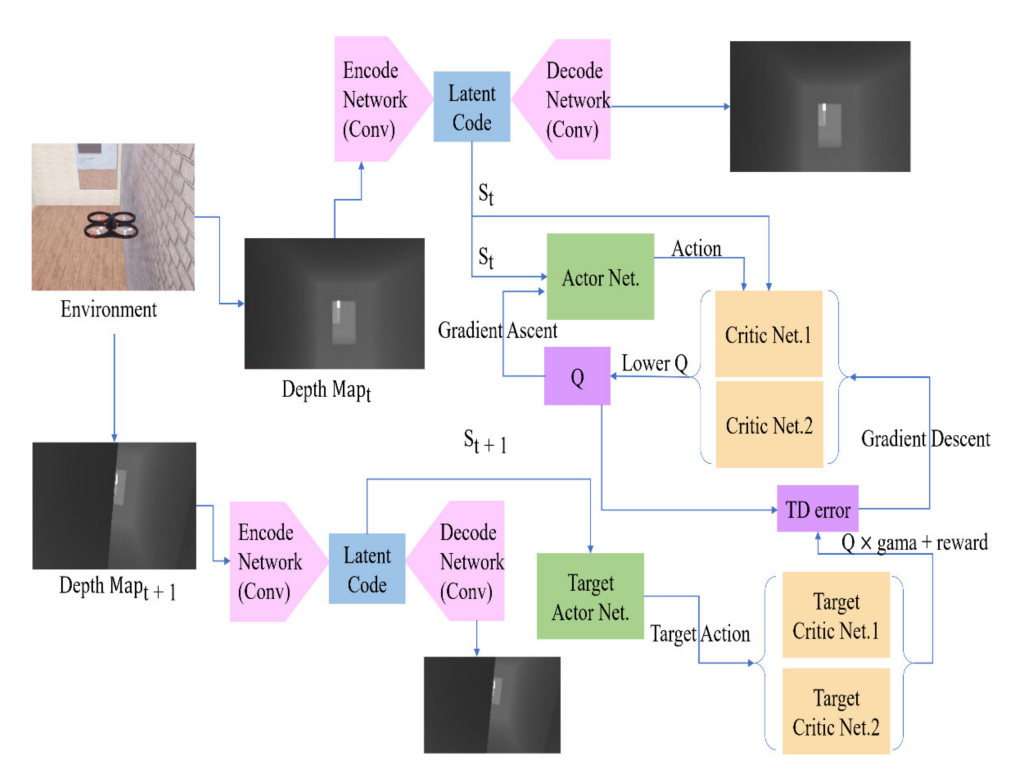
\includegraphics[scale=0.4]{partes/img/RL-training-process.png}
        \caption[Diagrama de flujo del proceso de entrenamiento utilizado en \textit{Vision Based Drone Obstacle Avoidance by Deep Reinforcement Learning}]{Diagrama de flujo del proceso de entrenamiento utilizado en \cite{Xue2021}.}
        \label{fig:rl-training-process}
    \end{figure}

    \par Métodos con información parcial del entorno tales como \cite{Zhang2019} utilizan la información conocida del entorno para planear trayectorias libres de colisión antes de la ejecución del vuelo (proceso denominado \textit{trajectory planning} o planeamiento de trayectorias), reduciendo la carga computacional del algoritmo durante la ejecución de la trayectoria, permitiendo que los recursos computacionales del dron estén disponibles para otras tareas. En particular, el método propuesto en \cite{Zhang2019}, genera una colección de trayectorias libres de colisión, y alterna entre las distintas trayectorias o \textit{lanes} al momento de ejecución, dependiendo de la información de los obstáculos observados, dándole la capacidad al dron de reaccionar a obstáculos no provistos en la información inicial del entorno. Sin embargo, el requerimiento de poseer información previa sobre el entorno hace que sea complicado que este método opere en entornos genéricos o desconocidos.

    \par Otros métodos utilizan redes neuronales convolucionales (\textit{CNN} del inglés \textit{convolutional neural networks}) para directa o indirectamente producir trayectorias libres de colisión en entornos desconocidos. **** En \cite{Yang2021} se utiliza una \textit{CNN} probabilística, que a partir de una cámara monocular genera mapas de profundidad y mapas de confianza probabilísticos, que posteriormente son utilizados para navegar arbitrariamente el entorno sin generar colisiones. Sin embargo, en \cite{Yang2021} la navegación es arbitraria, las trayectorias generadas no van dirigidas hacia ningún objetivo en particular, lo cual hace que sea de poca utilidad en la práctica.

    \par Los métodos que utilizan \textit{CNN} requieren una base de datos para su proceso de entrenamiento. Esto limita la gama de tareas que puede resolver una \textit{CNN} a las tareas para las cuales existe una base datos disponible, por ejemplo, se puede entrenar una \textit{CNN} para estimar imágenes de profundidad a partir de imágenes \textit{RGB} utilizando bases de datos como \textit{KITTI} \cite{Geiger2013} y \textit{TUM RGB-D} \cite{Sturm2012}. Las \textit{CNN} tienen la ventaja de que son relativamente sencillas de entrenar con respecto a otras alternativas (como el aprendizaje por reforzamiento), por lo cual resultan atractivas para resolver problemáticas en donde se tiene disponible una base de datos. Es importante destacar que actualmente no hay bases de datos generales enfocadas en la tarea de la evasión de obstáculos para drones, limitando el uso que se le puede dar a las \textit{CNN} dentro de esta problemática. 
    
    \par En \cite{Loquercio2021} se soluciona el requerimiento de poseer una base de datos para el entrenamiento de una \textit{CNN} como política de evasión de obstáculos; empleando el denominado entrenamiento por imitación (del inglés \textit{imitation learning}), en lugar de aplicar entrenamiento supervisado sobre una base de datos ya existente, se utiliza, dentro de un entorno de simulación, una política experta con acceso privilegiado a la información de los obstáculos del entorno (el ``experto'') para generar una base de datos de trayectorias libres de colisión. Esta base de datos contiene ejemplos de trayectorias libres de colisión dado una imagen de profundidad, mediciones inerciales del estado del dron y la dirección hacia donde se encuentra el objetivo del dron. Esto permite entrenar una política ``estudiante'' (modelada como una \textit{CNN}) de generación de trayectorias directa a partir de imágenes de profundidad, mediciones inerciales y una dirección objetivo. Una visión general del metodo se puede observar en la figura \ref{fig:agile-autonomy-overview}.

    \begin{figure}[H]
        \centering
        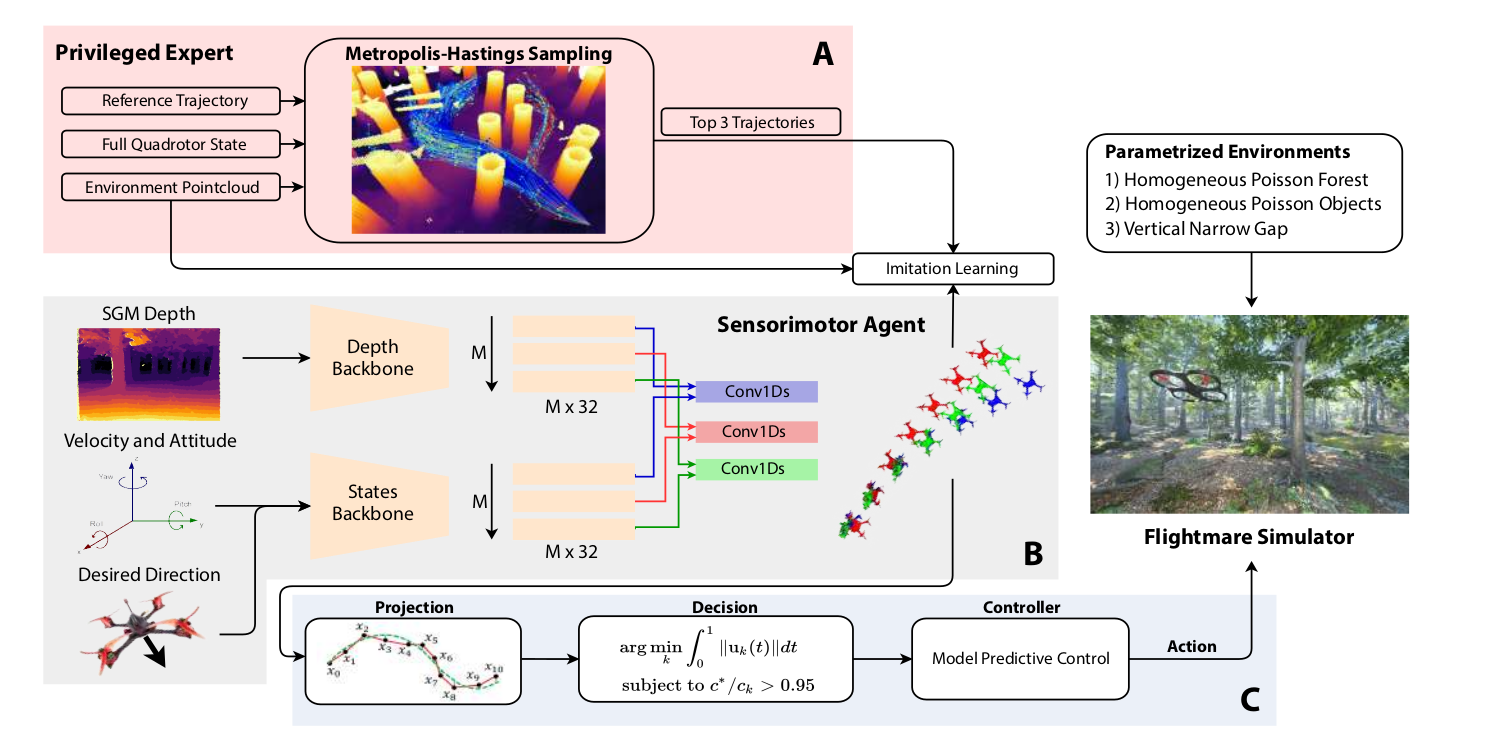
\includegraphics[scale=0.3]{partes/img/agile-autonomy-overview.png}
        \caption[Visión general del método del método utilizado en \textit{Learning high-speed flight in the wild}]{Visión general del método utilizado en \cite{Loquercio2021}. \textbf{(A)} El ``experto'' genera una distribución de trayectorias libre de colisión que siguen una trayectoria de referencia. Las trayectorias generadas están condicionadas por la completa información de obstáculos del entorno. \textbf{(B)} La política ``estudiante'' es entrenada mediante entrenamiento por imitación para predecir las mejores 3 trayectorias a partir una estimación de la profundidad, mediciones inerciales del dron y una dirección objetivo. \textbf{(C)} Las predicciones son proyectadas en el espacio de las trayectorias polinomiales y finalmente la trayectoria con el costo de predicción mas bajo es ejecutada por el modelo de control. }
        \label{fig:agile-autonomy-overview}
    \end{figure}
    
    La política ``estudiante'' puede transferirse trivialmente a un ambiente fuera de simulación, siempre y cuando al momento de generar la base datos de entrenamiento se utilicen métodos de estimación de imágenes de profundidad cuya salida posea niveles similares de ruido tanto en simulación como en entornos reales, tales como \textit{SGM} \cite{Hirschmüller2007} (del inglés \textit{semi global matching}). Finalmente  \cite{Loquercio2021} resulta bastante conveniente para la evasión de obstáculos pues, es sencillo de entrenar, la política ``estudiante'' se modela utilizando una \textit{CNN} ligera \cite{Howard2019} que no introduce demasiada latencia al momento de ejecución, no necesita información previa del entorno, es fácil de transferir para funcionamiento en ambientes fuera de simulación y toma en cuenta la dirección de objetivo del dron, lo cual produce trayectorias libres de colisión que se dirigen al objetivo.

\section{Justificación y planteamiento del problema}

    \par Los drones han experimentado un crecimiento exponencial en su adopción en diversas aplicaciones, desde la agricultura de precisión hasta la logística de entrega y la vigilancia. Sin embargo, uno de los desafíos fundamentales que enfrentan los drones es su capacidad para operar de manera segura y autónoma en entornos dinámicos y desconocidos, donde los obstáculos pueden surgir en cualquier momento y lugar. La evasión de obstáculos es esencial para garantizar la seguridad de las operaciones de los drones y su capacidad de navegación autónoma en entornos complejos.

    \par En este contexto, el presente trabajo se centra en la implementación de un algoritmo de evasión de obstáculos para drones, específicamente diseñado para abordar la falta de información a priori sobre la ubicación de los obstáculos. Este enfoque reactivo permitirá que los drones tomen decisiones en tiempo real para evitar obstáculos de manera segura y eficiente, lo que es esencial para su aplicación en entornos urbanos, industriales y otros escenarios realistas.

    \par La empresa ACSL (del inglés \textit{Autonomous Control Systems Laboratory}), con sede en Japón, se ha destacado como líder en la investigación y desarrollo de soluciones de control autónomo para drones. ACSL ha identificado la necesidad crítica de mejorar la capacidad de los drones para evadir obstáculos de manera efectiva, lo que impulsará la seguridad de las operaciones y abrirá nuevas oportunidades de aplicación en una variedad de industrias.

    \par La implementación exitosa de un algoritmo de evasión de obstáculos reactivo tiene el potencial de revolucionar la seguridad y la autonomía de los drones, lo que beneficiaría a una amplia gama de industrias, desde la entrega de paquetes hasta la inspección de infraestructuras críticas. Además, contribuirá al liderazgo continuo de ACSL en el campo de la tecnología de drones, consolidando su posición como un actor clave en la innovación y desarrollo de soluciones de vanguardia en Japón y a nivel internacional.
        
   
\section{Objetivos}

    \subsection{Objetivo general}
    
    Implementar un algoritmo de evitación de obstáculos para drones autónomos y realizar
    pruebas de dicha implementación tanto en entorno de simulación como en el campo.
    
    \subsection{Objetivos específicos}
    
    \begin{itemize}
        \item Investigar el estado del arte de los algoritmos de evitación de obstáculos para drones autónomos.
        \item Implementar un algoritmo de evitación de obstáculos para drones autónomos sobre un ambiente de simulación y realizar pruebas en dicho ambiente.
        \item Ajustar la implementación del algoritmo seleccionado al hardware de un dron autónomo realizando las optimizaciones necesarias y realizar pruebas de campo de dicha implementación.
    \end{itemize}

\section{Estructura del trabajo}

    \par Este trabajo se encuentra dividido en seis capítulos de la siguiente manera:
    
    \par El \textbf{capítulo 1} es el ya presentado e incluye: la introducción, planteamiento del problema, justificación, los antecedentes que motivaron la realización del trabajo y se listan los objetivos.

    \par El \textbf{capítulo 2} describe la empresa receptora en donde se realizó este trabajo, el Laboratorio de Sistemas de Control Autónomo (ACSL, del inglés \textit{Autonomous Control Systems Laboratory}), localizado en Tokio, Japón. 
    
    
    \par En el \textbf{capítulo 3} se explican las bases teóricas de los principales algoritmos utilizados en este trabajo. 
    
    \par El \textbf{capítulo 4} incluye la revisión del estado del arte sobre los métodos de evasión de obstáculos para drones autónomos. 
 
    \par El \textbf{capítulo 5} muestra la implementación del algoritmo de evitación de obstáculos y la arquitectura utilizada.
    
    \par En el \textbf{capítulo 6} se muestran y se discuten los resultados obtenidos.
    
    \par Finalmente en el \textbf{capítulo 7} se presentan las conclusiones del presente trabajo, así como las recomendaciones para posibles trabajos futuros. 

\chapter{Descripción de la empresa receptora}
\label{capitulo2}
\lhead{Capítulo 2. \emph{Descripción de la empresa receptora}}

La empresa donde se realizo este trabajo es el Laboratorio de Sistemas de Control Autónomos, ACSL (del inglés \textit{Autonomous Control Systems Laboratory}), en la sede de Tokio, Japón. El logo de la organización se muestra en la figura \ref{fig:acsl-logo}. ACSL fue fundada en el año 2013 y tiene como visión revolucionar la infraestructura social mediante la aplicación de tecnología robótica.

\begin{figure}[H]
    \centering
    
\includegraphics[scale=0.25]{partes/img/logo-acsl.jpg}
    \caption[Logo de ACSL (\textit{Autonomous Control Systems Laboratory})]{Logo de ACSL (\textit{Autonomous Control Systems Laboratory})}
    \label{fig:acsl-logo}
\end{figure}

ACSL cuenta con distintos productos sobre los cuales se desarrollan distintas soluciones. En particular, ACSL domina el desarrollo de vehículos aéreos no tripulados, ofreciendo una gama amplia de productos todos desarrollados y ensamblados en Japón. En la figura \ref{fig:acsl-products} se muestran y describen algunos de estos productos, entre ellos SOTEN, el producto en el cual se implementó el presente trabajo.

\begin{figure}
    \centering
    \begin{subfigure}[b]{0.45\textwidth}
        \centering
        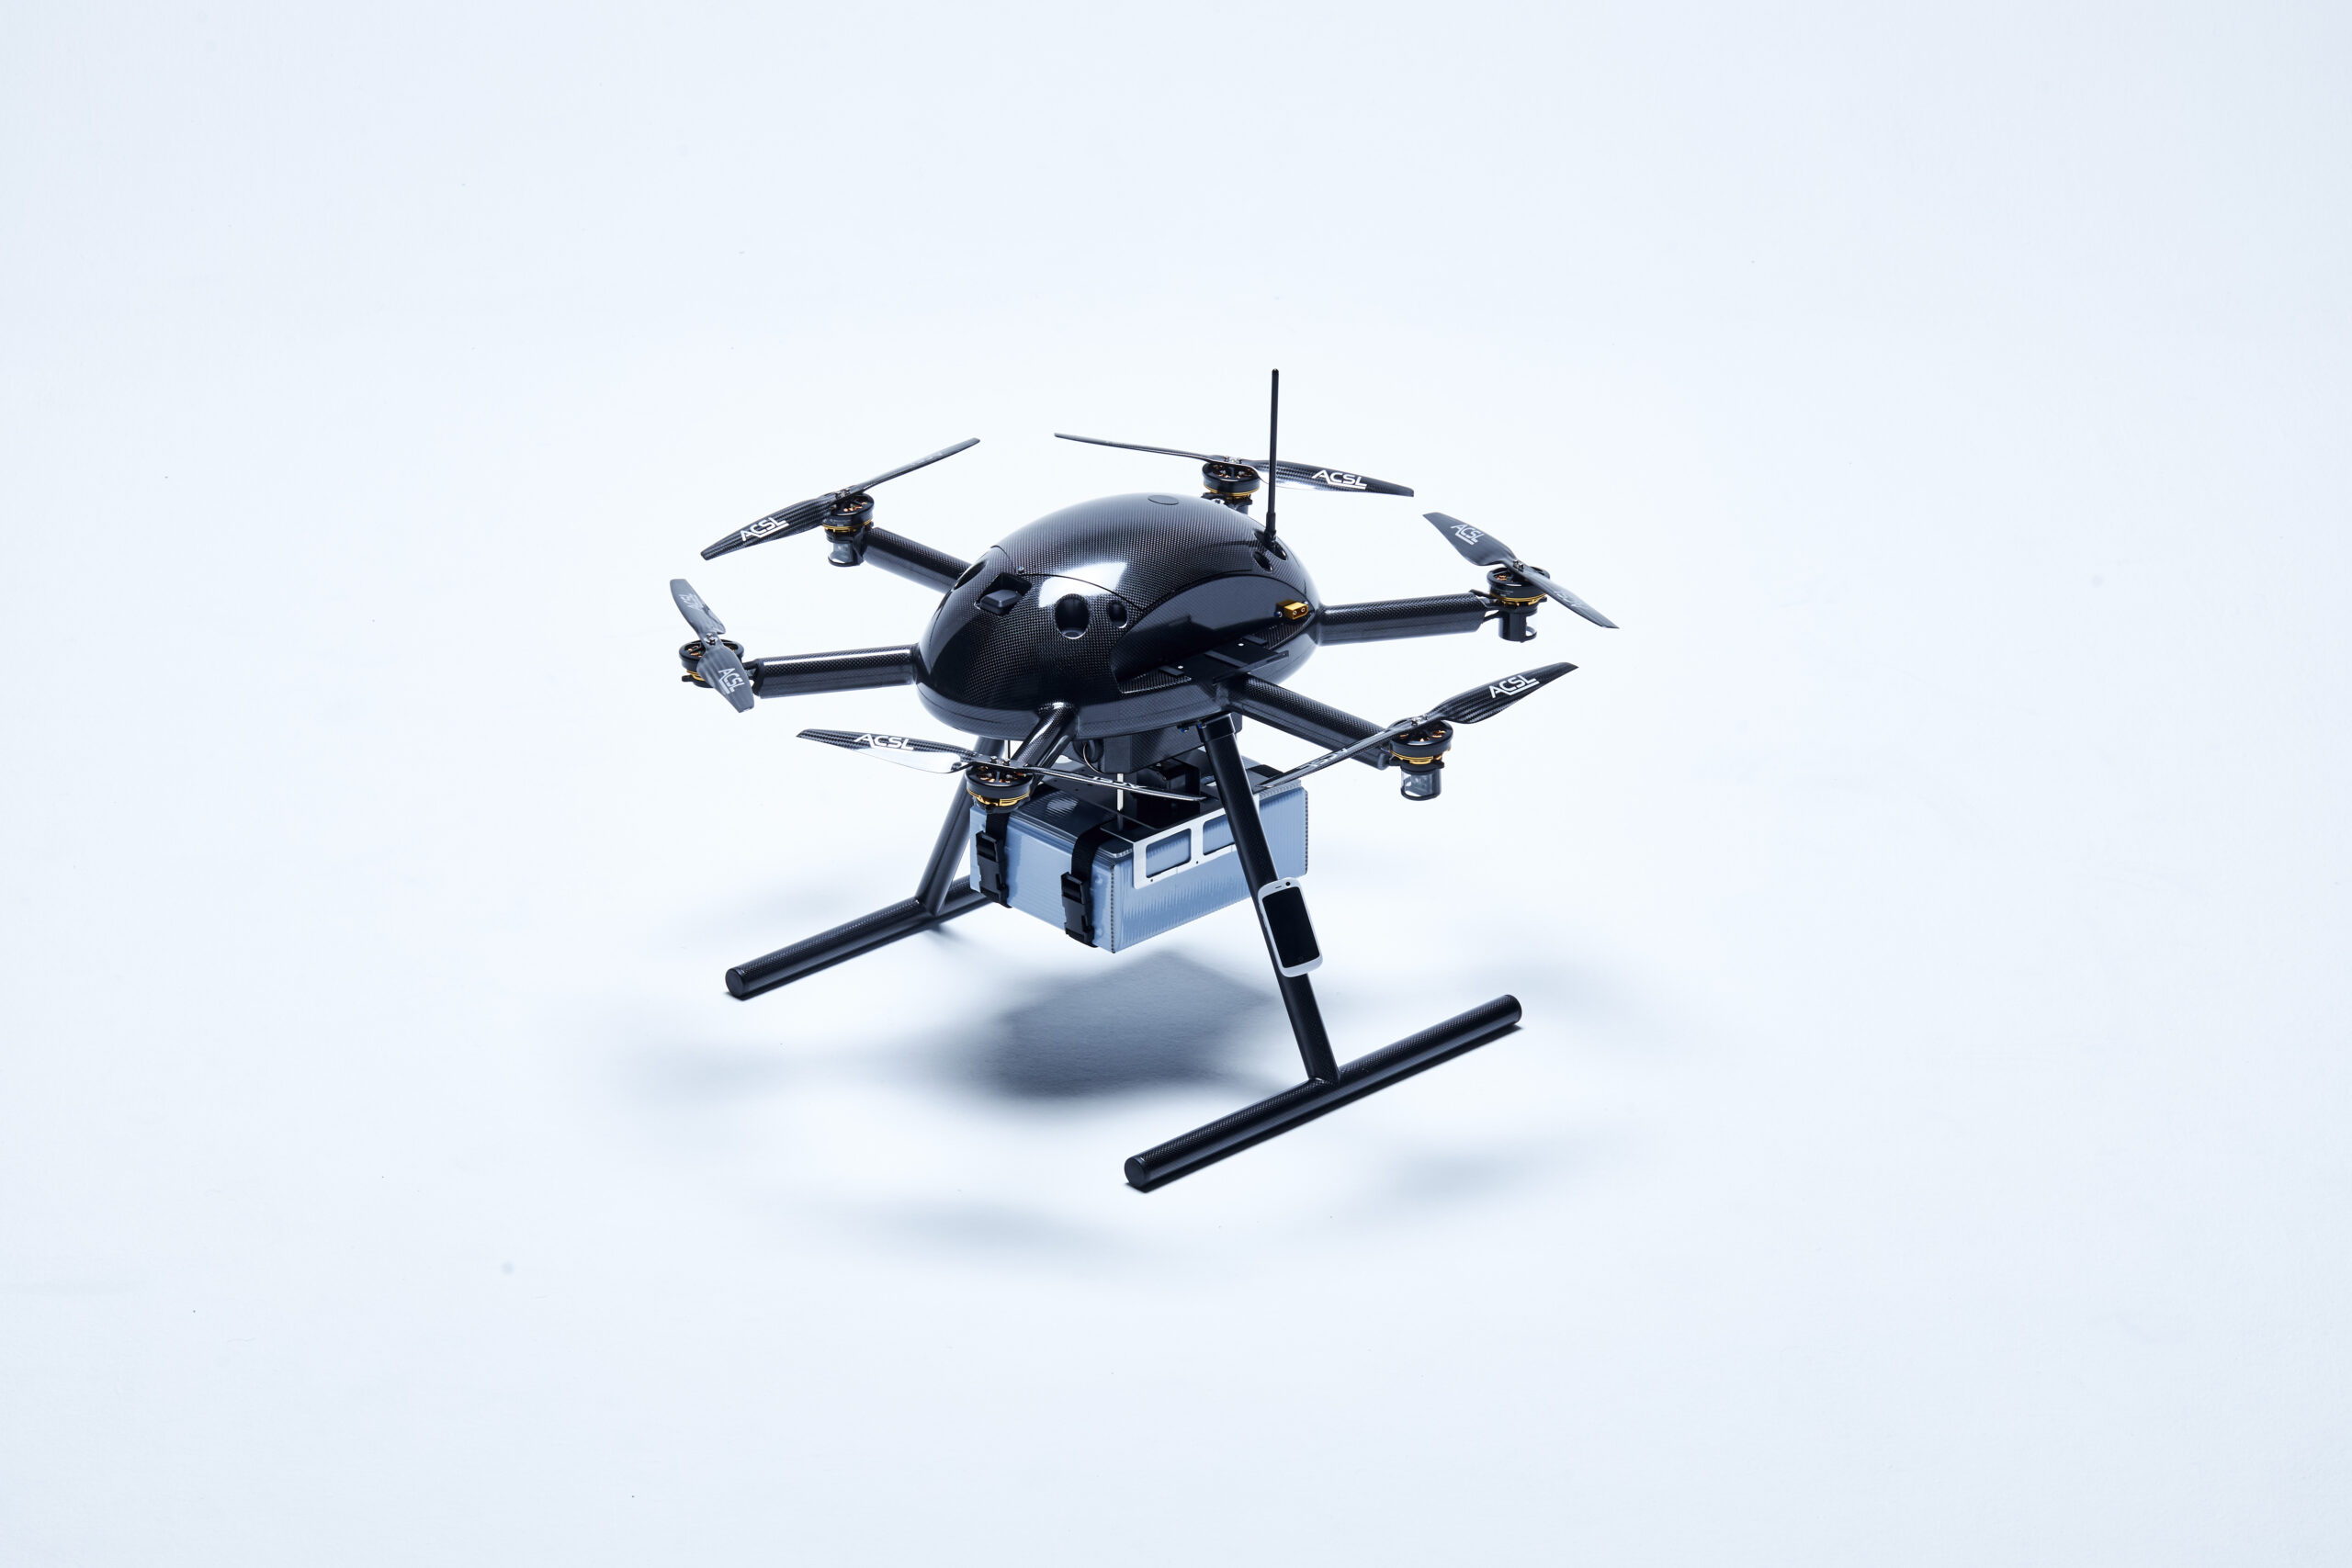
\includegraphics[width=\textwidth]{partes/img/PF2.jpg}
        \caption{PF2}
        \label{fig:pf2}
    \end{subfigure}
    \hfill
    \begin{subfigure}[b]{0.45\textwidth}
        \centering
        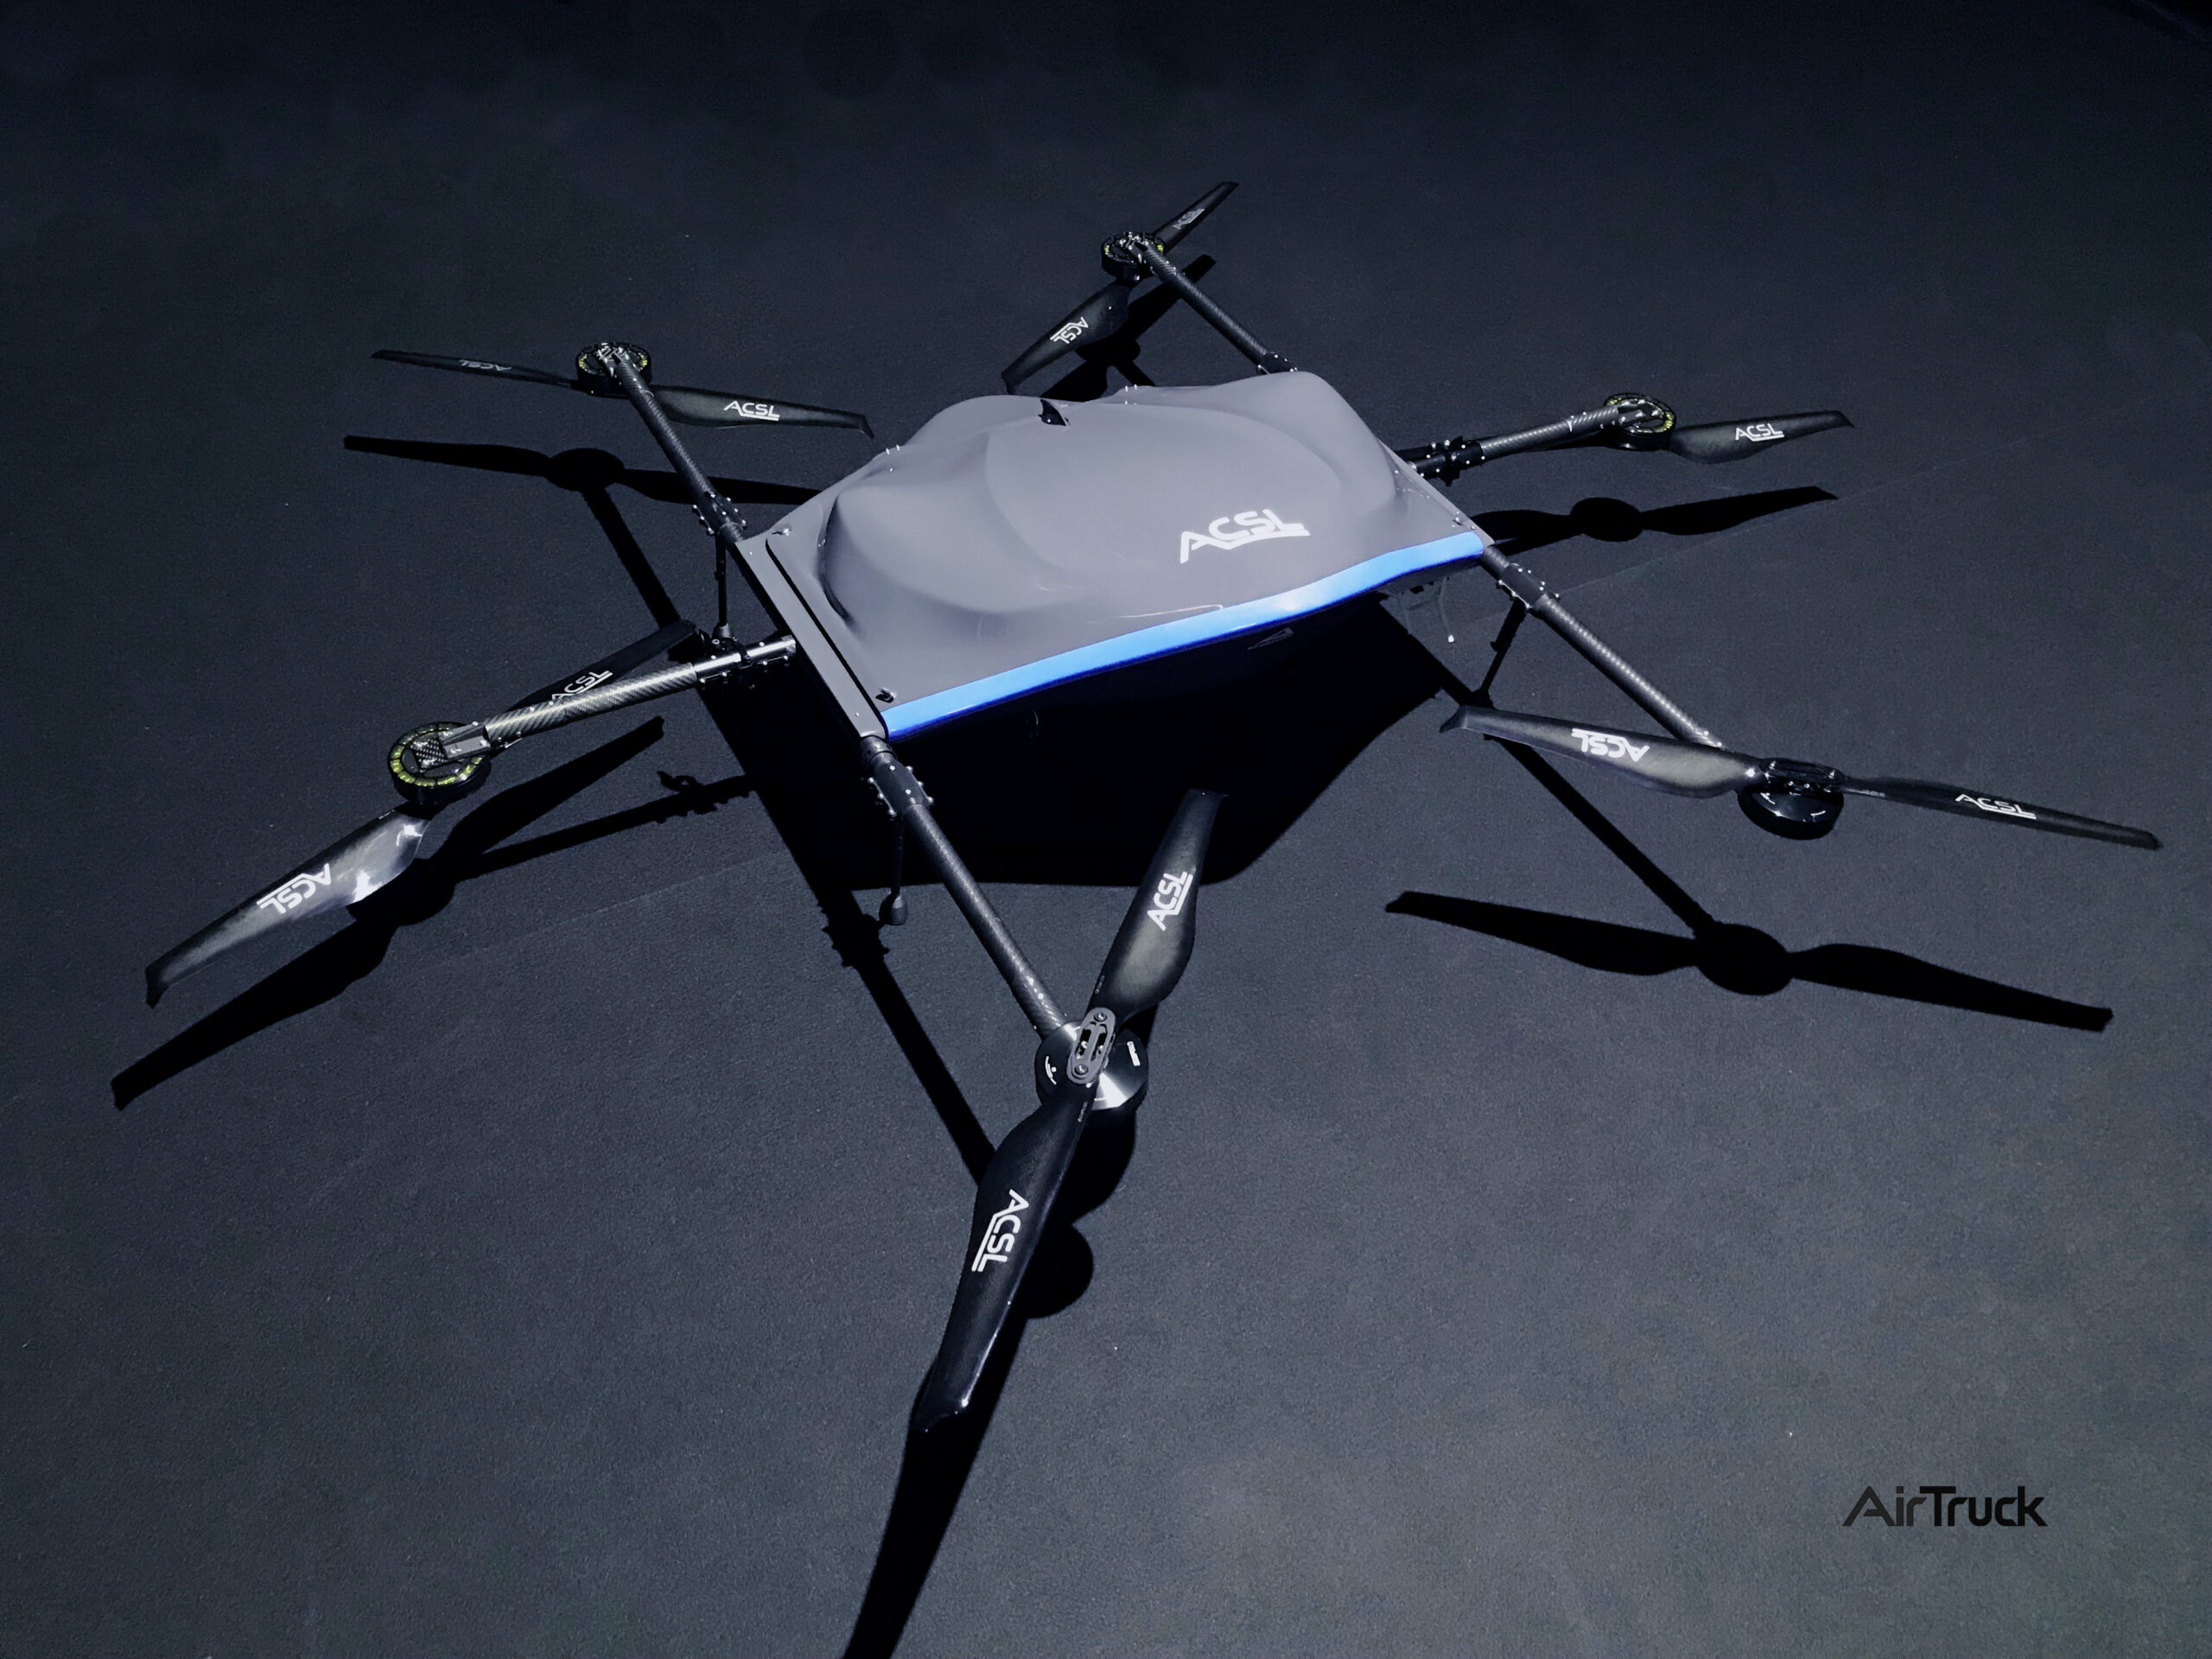
\includegraphics[width=\textwidth]{partes/img/AirTruck.jpg}
        \caption{AirTruck}
        \label{fig:AirTruck}
    \end{subfigure}
    \break
    \begin{subfigure}[b]{0.45\textwidth}
        \centering
        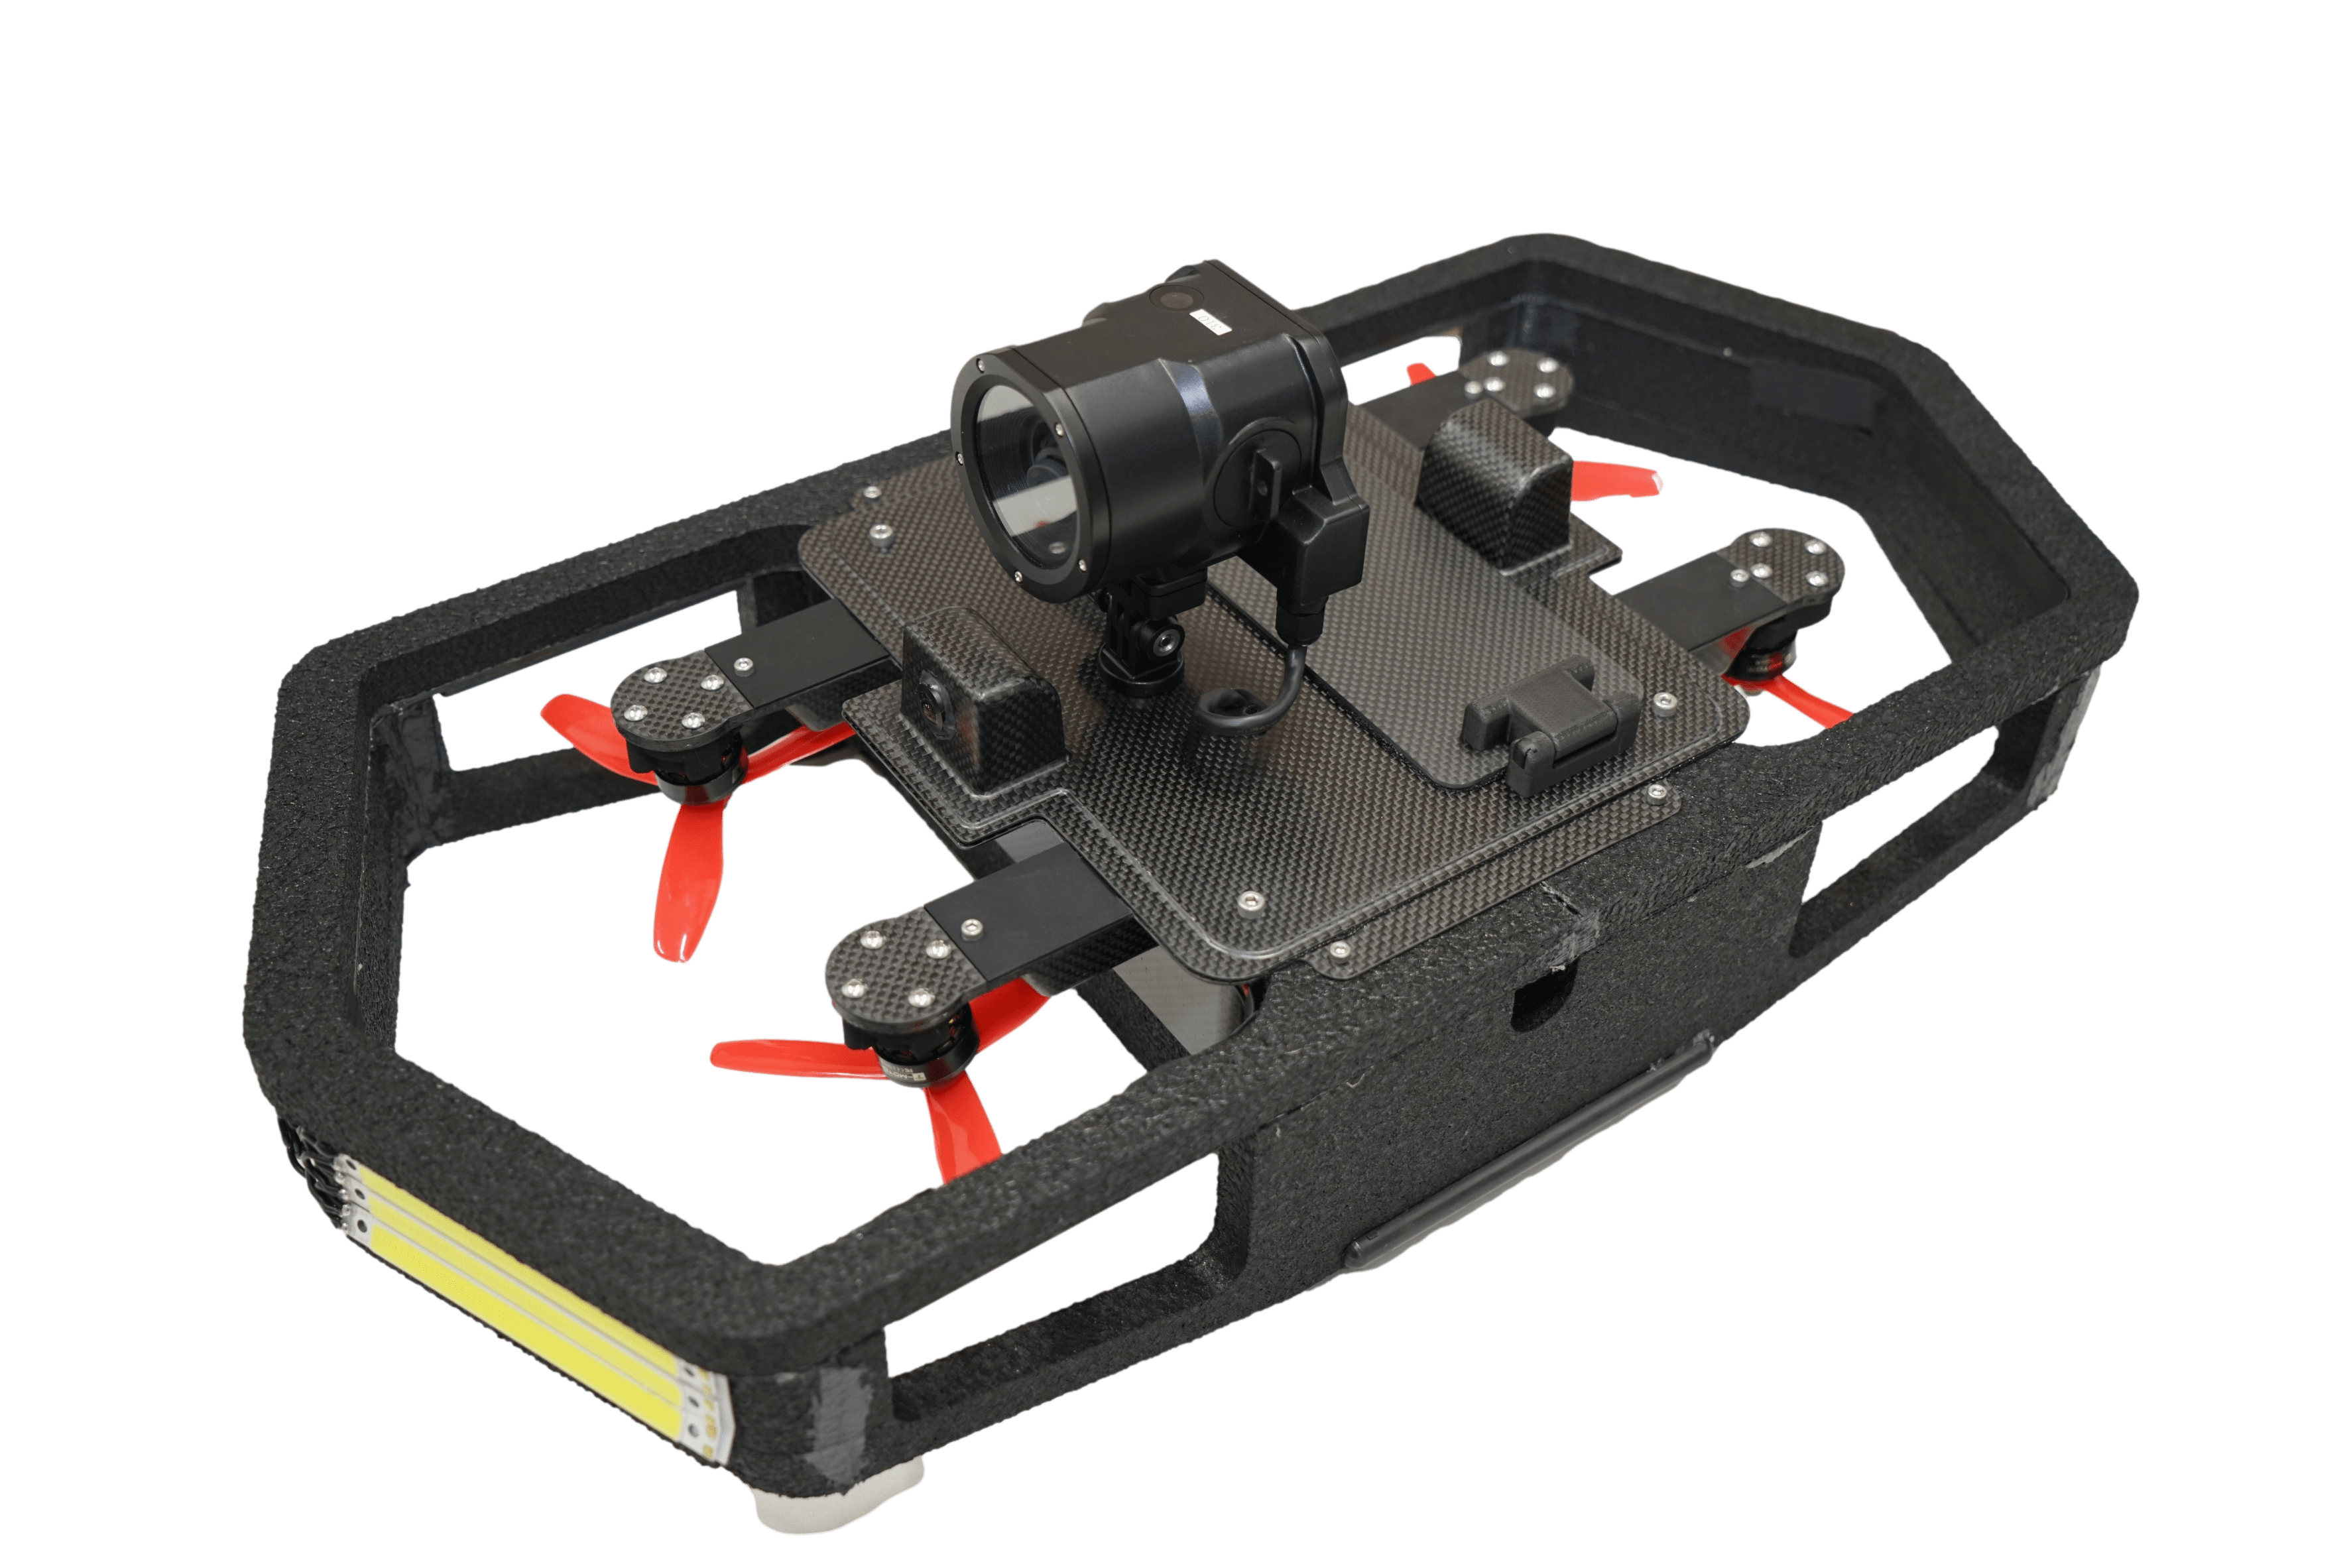
\includegraphics[width=\textwidth]{partes/img/Fi4.png}
        \caption{Fi4}
        \label{fig:Fi4}
    \end{subfigure}
    \hfill
    \begin{subfigure}[b]{0.45\textwidth}
        \centering
        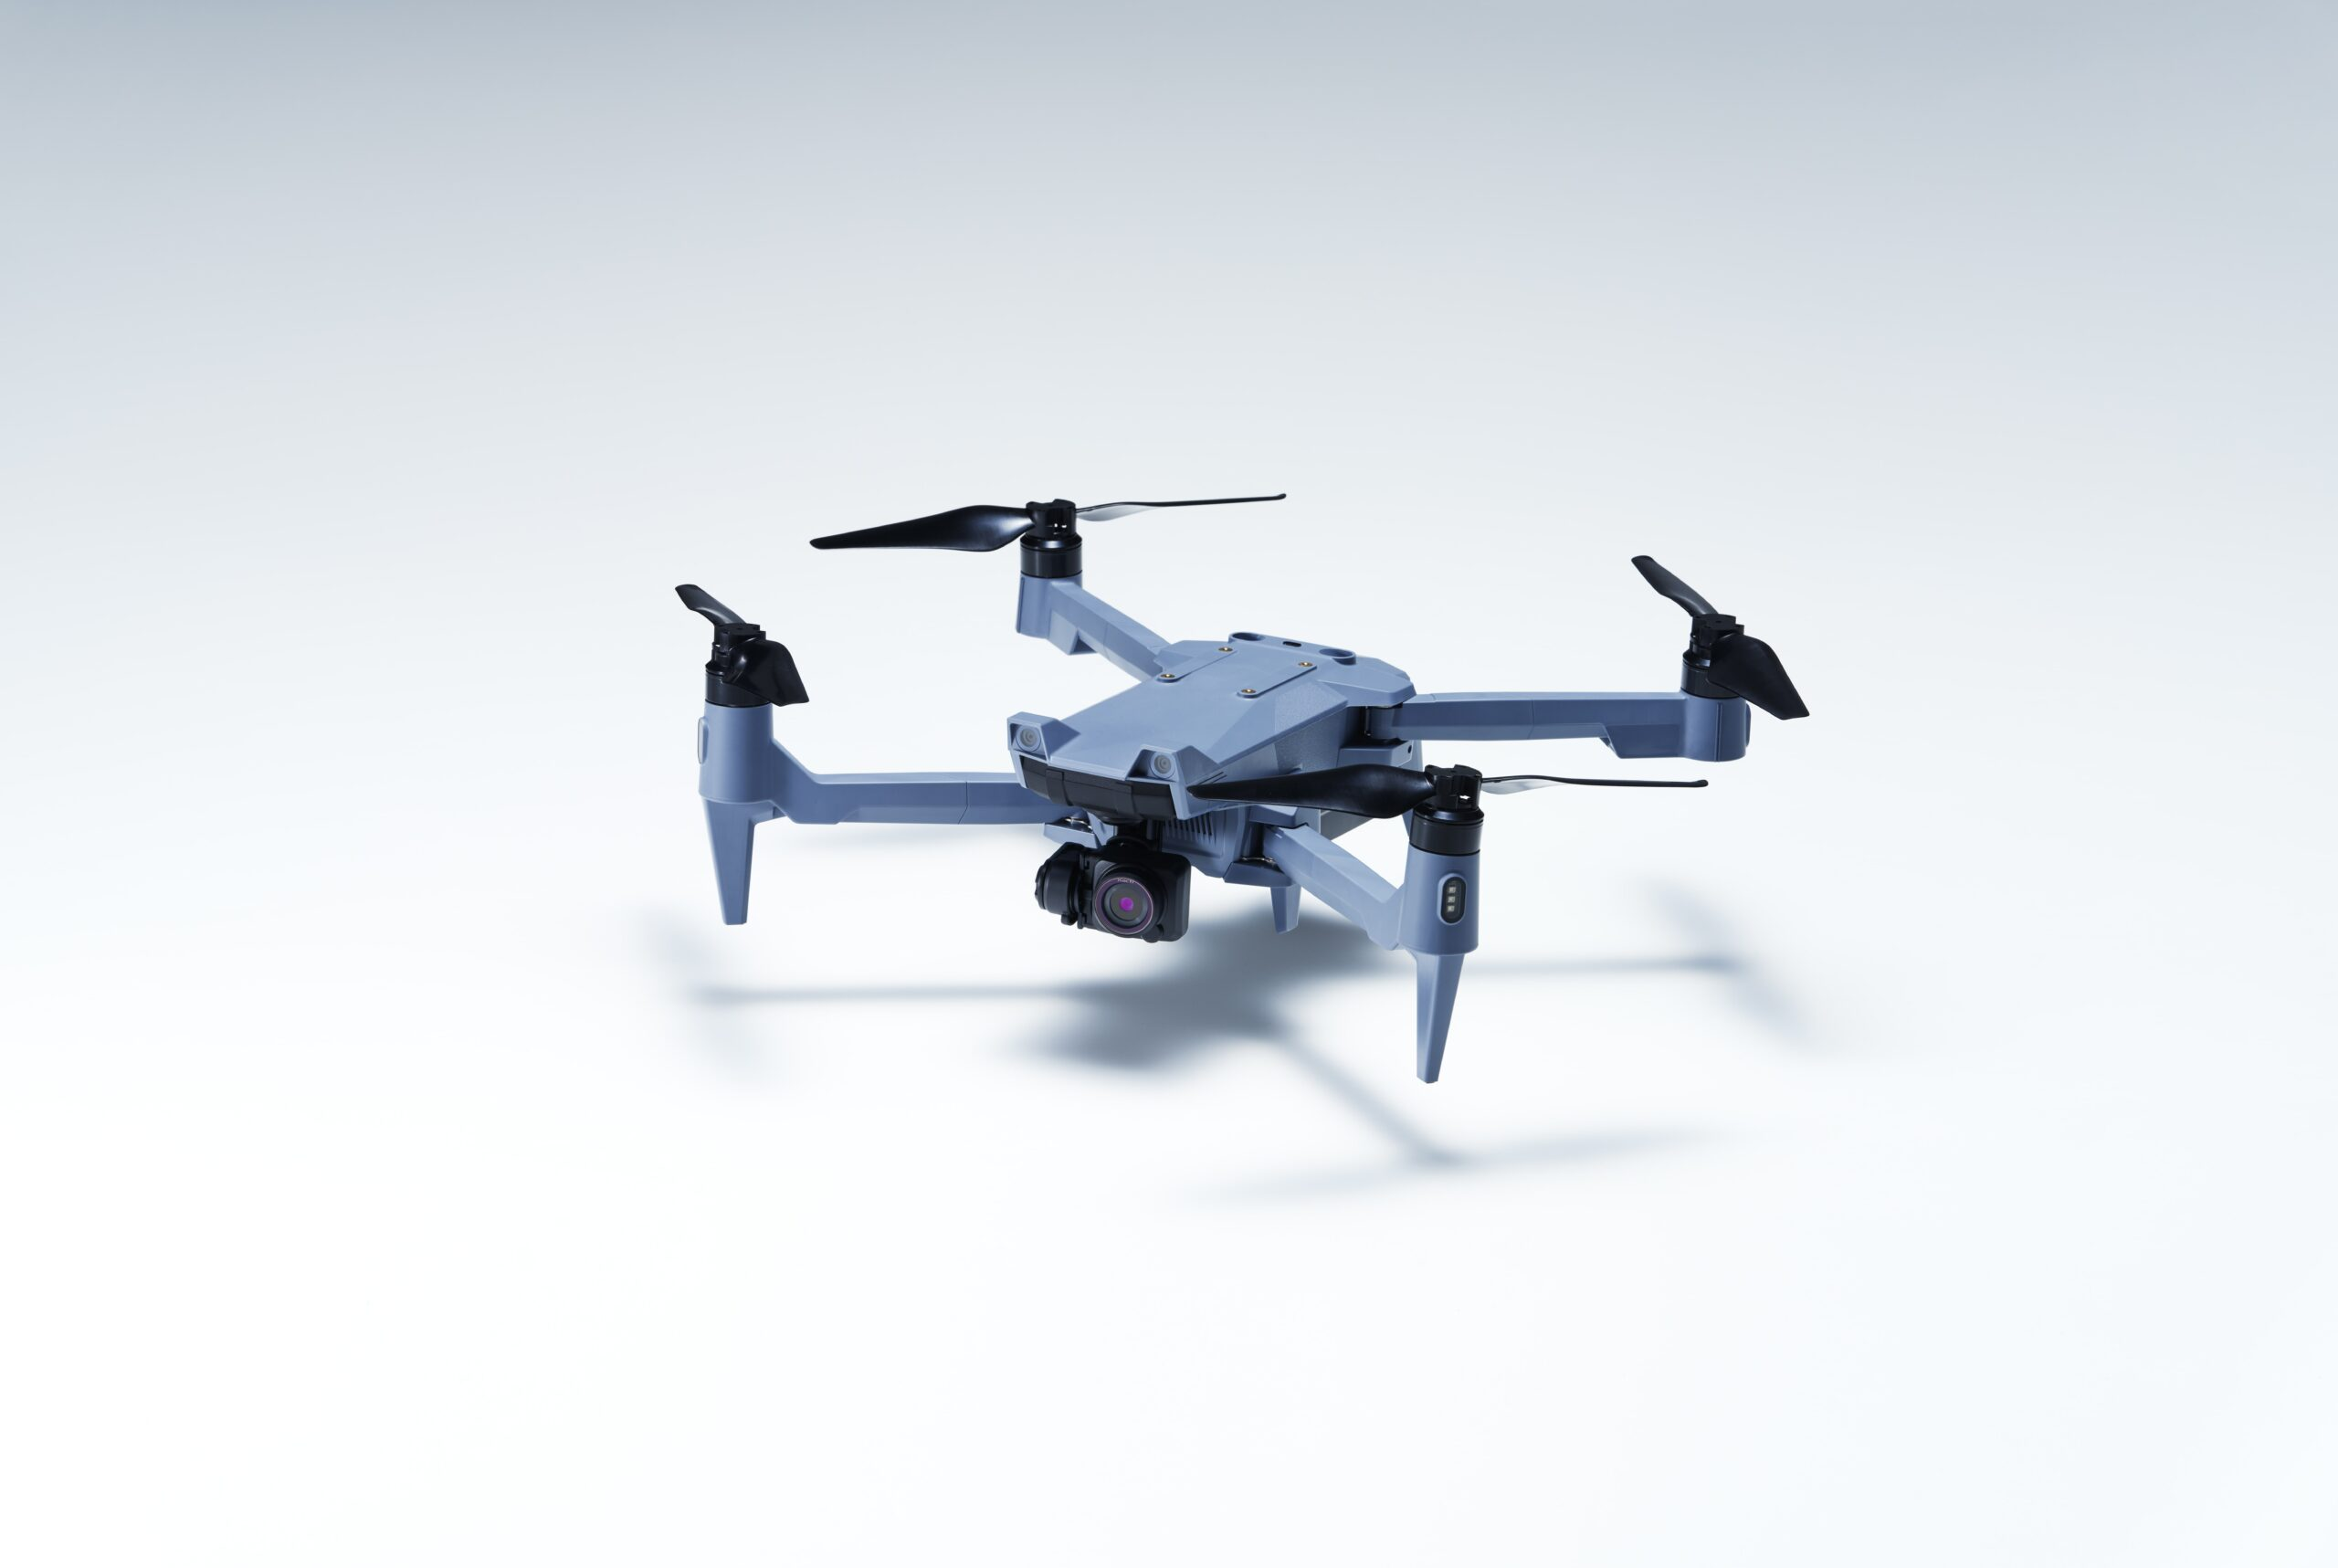
\includegraphics[width=\textwidth]{partes/img/SOTEN.jpg}
        \caption{SOTEN}
        \label{fig:SOTEN_ACSL}
    \end{subfigure}
    \hfill
    
    \caption [Algunos productos de ACSL]{Algunos productos de ACSL. \textbf{(a)} \textbf{PF2}: Un dron con capacidad autónoma de seis rotores utilizado para aplicaciones de entrega de paquetes (\textit{delivery}), inspección y patrullaje en desastres naturales. \textbf{(b)} \textbf{AirTruck}: Un dron autónomo de seis rotores con capacidad de carga y vuelo superior utilizado para operaciones de logística. \textbf{(c)} \textbf{Fi4}: Un dron autónomo dedicado a la inspección de espacios confinados (tuberías, ductos de ventilación, entre otros). \textbf{(d)} \textbf{SOTEN}: Un dron pequeño de cuatro rotores dedicado a la fotografía aérea con capacidad autónoma utilizado para tareas de inspección, vigilancia y rescate. }
    \label{fig:acsl-products}
\end{figure}


Este trabajo se desarrolló bajo la supervisión del Equipo de Inteligencia de Máquinas (del inglés \textit{Machine Intelligence Team}) de ACSL, contando con Niklas Bergstroem, lider del Equipo de Inteligencia de Máquinas, como encargado de asesorar el desarrollo del trabajo. Gracias a los miembros del Equipo de Inteligencia de Máquinas de ACSL, este trabajo pudo ser desarrollado e implementado haciendo el uso de las plataformas y recursos disponibles.

\chapter{Marco teórico}
\label{capitulo3}
\lhead{Capítulo 3. \emph{Marco teórico}}

El presente capítulo tiene como intención exponer las bases teóricas necesarias para el desarrollo de este trabajo. Este capítulo se divide en cuatro secciones: la Sección \ref{sec:teo-uav} explica la teoría relacionada con el modelo de los vehículos aéreos no tripulados (UAV, del inglés \textit{unmanned aerial vehicle}), en particular, los UAV de cuatro rotores; la Sección \ref{sec:teo-stereo} describe el funcionamiento de los algoritmos utilizados para la obtención de mapas de profundidad a partir de un sistema de visión estereoscópica; la Sección \ref{sec:teo-neural} explica la teoría relacionada con las redes neuronales y Redes Neuronales Convolucionales (CNN, del inglés \textit{Convolutional Neural Networks}); finalmente, la Sección \ref{sec:teo-interprocess} describe el funcionamiento de los protocolos de comunicación entre procesos utilizados en este trabajo.

\section{Vehículos aéreos no tripulados de cuatro rotores}
\label{sec:teo-uav}

Un vehículo aéreo no tripulado de cuatro rotores, también llamado \textit{Quadrotor} UAV (abreviado QUAV a efectos de este trabajo) es una aeronave no tripulada propulsada por cuatro rotores que es controlada por un operador en tierra. Los QUAVs pertenecen a la familia de los drones y su principal característica es que la configuración de los cuatro rotores les permite rotar y elevarse independientemente mediante control de la velocidad de rotación de los rotores \cite{multidrone2017review}; el mismo mecanismo les permite moverse omni-direccionalmente, así como también flotar en sitio (del inglés \textit{hovering in place}). Debido a que su funcionamiento es enteramente dependiente del empuje producido los rotores, los QUAVs generalmente tienen un tiempo de vuelo máximo bastante reducido (menos de 30 minutos en promedio \cite{multidrone2017review}), pues baterías de alta capacidad de carga introducen peso en el sistema que puede afectar considerablemente la capacidad de vuelo del vehículo; sobre esta misma linea, el limite de masa de carga de estos vehículos es generalmente bastante pequeño. Estas características de los QUAVs hacen que su uso sea atractivo para aplicaciones donde la agilidad es un factor importante, siempre y cuando la capacidad de carga necesaria sea relativamente baja y tiempos de vuelo inferiores a 30 minutos sean aceptables \cite{multidrone2017review}. En el Capítulo \ref{capitulo2}, en la Figura \ref{fig:acsl-products} se muestra SOTEN, un QUAV diseñado por ACSL para aplicaciones de fotografía aérea (inspección, vigilancia, entre otras) y que sirve de plataforma física para el desarrolo del presente trabajo. Con la finalidad de comprender la estructura y condiciones de arquitectura de la plataforma física, a continuación se da una breve descripción de los componentes de un QUAV. 

\subsection{Componentes}

La configuración de componentes general de los QUAVs, si bien bastante amplia y llena de excepciones, cuando se remiten a los QUAVs comerciales, se puede englobar en: Un conjunto de sensores, que se utilizan principalmente para localizar el vehículo en el entorno; una unidad de control de vuelo (FCU, del inglés \textit{Flight Control Unit}), encargada de controlar la velocidad de rotación de los rotores; al menos una computadora a bordo (\textit{Onboard PC} en inglés), que se encarga de realizar el procesamiento necesario para llevar a cabo tareas de alto nivel, como la evasión de obstáculos y el mapeo del entorno; y una estación de control en tierra (GCS, del inglés \textit{Ground Control Station}) \cite{multidrone2017review}. 

\subsubsection{Sensores}
\label{sec:QUAV-sensors}

Es de vital importancia que un QUAV tenga la capacidad de estimar su estado (orientación, altitud, posición y velocidad) utilizando solamente los componentes disponibles a bordo del vehículo. Para la estimación de orientación se utiliza una unidad de mediciones inerciales \cite{multidrone2017review} (IMU, del inglés \textit{Inertial Measurement Unit}) que se compone de un acelerómetro y giroscopio, ambos midiendo sus cantidades con respecto al marco de referencia del cuerpo del vehículo. Adicionalmente, también se puede utilizar un magnetómetro (brújula), para obtener la información de la orientación del vehículo con respecto al norte magnético del planeta tierra. Utilizando la información del IMU y del magnetómetro, el FCU puede estimar la orientación del cuerpo del vehículo con un nivel de precisión aceptable \cite{multidrone2017review}. 

Para la estimación de posición y velocidad se puede emplear localización visual utilizando algoritmos de localización y mapeo con cámaras estereoscópicas o LiDAR \cite{multidrone2017review}. Estos algoritmos pueden llegar a tener limitaciones considerables cuando las condiciones de iluminación no son ideales y su rendimiento en entornos al aire libre es limitado debido a la uniformidad de las texturas del entorno \cite{multidrone2017review}. Alternativamente se puede utilizar GPS (del inglés \textit{Global Postionaing System}) para la localización a partir de señales de satélite \cite{multidrone2017review}; en este esquema la posición es estimada mediante triangulación entre el vehículo y un sistema de satélites, la velocidad es estimada utilizando el efecto \textit{doppler} y la altitud se estima utilizando un barómetro (sensor de presión atmosférica) o un sistema sonar \cite{multidrone2017review}. La localización por GPS es bastante efectiva para su uso en entornos al aire libre, pero no es posible utilizarlo en aplicaciones que naveguen en interiores debido al requerimiento de tener recepción de las señales de los satélites. Es común que un QUAV tenga acceso tanto a localización por visión como a localización por GPS, alternando entre ambas dependiendo de las condiciones de iluminación y recepción del satélite.

\subsubsection{FCU}
\label{sec:QUAV-FCU}

Este componente maneja la estimación del estado del QUAV a partir de las señales de los sensores, así como el cálculo de las acciones de control para mantener estabilidad durante el vuelo. El FCU ofrece distintos modos de control, desde asistencia de orientación, asistencia en posición y asistencia de velocidad; todos estos con la finalidad de que controlar el QUAV en alto nivel sea una tarea más sencilla tanto para un operador como para otro algoritmo de alto nivel (como la evasión de obstáculos, el caso de este trabajo). 

\subsubsection{Computadora a bordo}

Ejecuta los algoritmos de alto nivel que requieren más poder de cómputo para su procesamiento, tales como algoritmos de localización por visión, inferencia con redes neuronales, procesamiento y \textit{broadcasting} de imágenes, mapeo del entorno, entre otros. Algunas se equipan con unidades de procesamiento gráfico (GPU, del inglés \textit{Graphics Processing Unit}) que contribuyen en la aceleración de las operaciones de procesamiento distribuido o de inferencia de redes neuronales, en ambos casos utilizando tecnologías como CUDA (Arquitectura Unificada de Dispositivos de Cómputo, del inglés: \textit{Compute Unified Device Architecture}). La solución propuesta en el presente trabajo se implementa y ejecuta justamente dentro de la computadora a bordo del QUAV.

\subsubsection{GCS}

Estación de control en el suelo, permite que el operador en suelo coordine las operaciones que hace el QUAV, en otras palabras, sirve de interfaz de alto nivel entre el operador y las funciones implementadas en el QUAV. Usualmente se utiliza para planificar vuelos autónomos, monitorizar el estado de los sensores, realizar \textit{streaming} de las imágenes de los sensores visuales del vehículo (cámaras), lanzar rutinas de control como aterrizaje o despegue automático, así como también instrucciones especificas de la aplicación (por ejemplo, entregar paquete para QUAV orientado a \textit{delivery}).

En la Figura \ref{fig:QUAV-components} se muestra el diagrama de comunicación general de los componentes de un QUAV, además de los componentes descritos anteriormente, se muestra la interacción con el radio control que es controlado por el operador, este además de encargarse de la transmisión de los comandos de operación vía señales de radio, se puede utilizar para operar el vehículo directamente o en conjunción con la GCS para orquestar operaciones complejas. 

\begin{figure}[H]
    \centering
    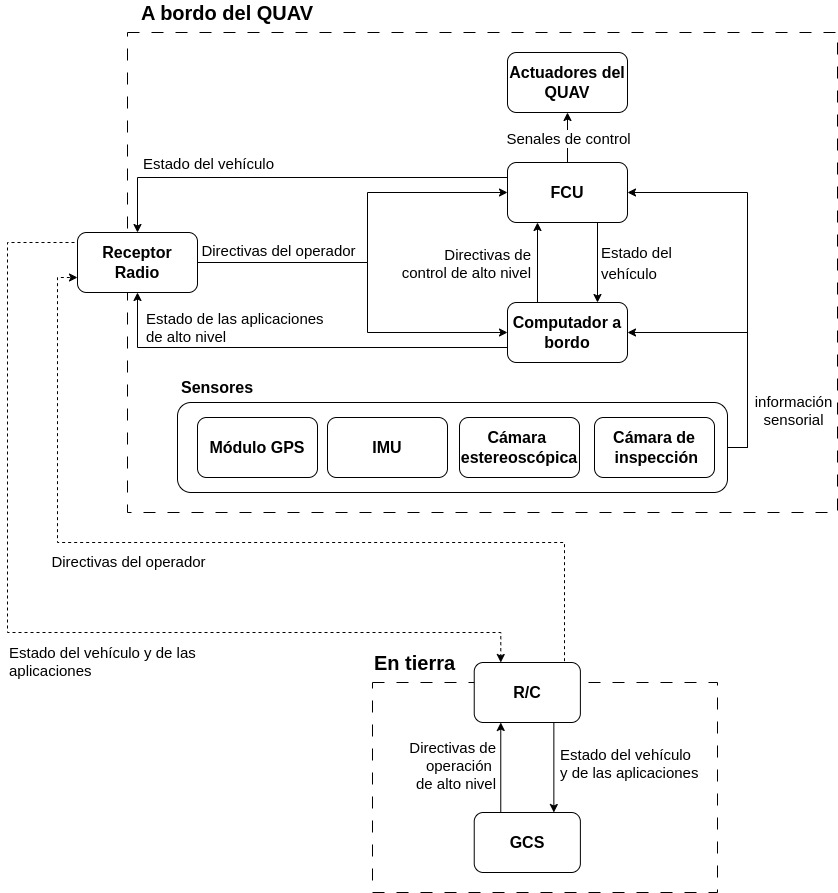
\includegraphics[scale=0.45]{partes/img/QUAV-components.jpg}
    \caption[Diagrama de comunicación general del los componentes de un QUAV.]{Diagrama de comunicación general del los componentes de un QUAV.} 
    \label{fig:QUAV-components}
\end{figure}

\subsection{Información relevante del modelo del QUAV}

En este trabajo no se hace una revisión completa del modelo cinemático y dinámico de un QUAV, sin embargo, es necesario discutir algunos conceptos que son utilizados en el desarrollo e implementación del algoritmo de evasión de obstáculos.

\subsubsection{Sistemas de referencia}

Existen dos sistemas de referencia de interés para el manejo de QUAV: el sistema de referencia inercial \jim{E}, usualmente anclado a la superficie de la tierra; y el sistema de referencia del cuerpo del vehículo \jim{B}, que se encuentra anclado a centro del marco del QUAV. Tal como se aprecia en la Figura \ref{fig:QUAV-model}, la rotación del sistema del cuerpo \jim{B}, es representada por \jim{\phi,\theta,\psi} \cite{multidrone2015modeling}, donde: \jim{\phi} es denominado rolido \textit{roll} y representa la rotación con respecto al eje inercial \jim{x}; \jim{\theta} es denominado \textit{pitch} y representa la rotación con respecto al eje inercial \jim{y}; y \jim{\psi} es denominado \textit{yaw} y representa la rotación con respecto al eje inercial \jim{z}. Por convención, la velocidad lineal del vehículo \jim{V_B} se expresa en el sistema \jim{B}.

\begin{figure}[H]
    \centering
    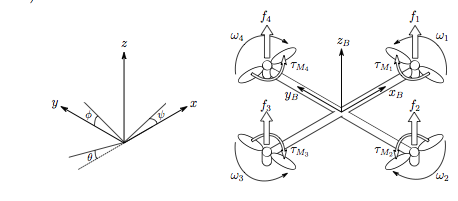
\includegraphics[scale=0.65]{partes/img/QUAV-model.png}
    \caption[Diagrama de un QUAV.]{Diagrama de un QUAV \cite{multidrone2015modeling}.} 
    \label{fig:QUAV-model}
\end{figure}

Es necesario establecer una transformación entre \jim{B} y \jim{E}, para ello podemos derivar una matriz de rotación a partir de rotaciones sucesivas dadas por \jim{\phi,\theta,\psi}, este tipo de transformación obtenida a partir de rotar \jim{\phi,\theta,\psi} se denomina transformación por ángulos de Euler \cite{eulerAngles}, se dice que \jim{\phi,\theta,\psi} son los ángulos de Euler que representan la rotación de \jim{B} con respecto al marco inercial \jim{E}.

La matriz de transformación por ángulos de Euler se obtiene por realizar las rotaciones sucesivas en el orden \textit{yaw}, \textit{pitch}, \textit{roll} \cite{multidrone2015modeling}, esto es:

\begin{itemize}
    \item {
        Rotar positivamente \jim{\psi} alrededor del eje \jim{z}.

        \begin{equation}
            \label{eq:euler-yaw}
            R_{\psi} = 
                \begin{bmatrix}
                    \cos{\psi} & \sin{\psi} & 0 \\
                    -\sin{\psi} & \cos{\psi} & 0 \\
                    0 & 0 & 1 
                \end{bmatrix}
        \end{equation}
    }

    \item {
        Rotar positivamente \jim{\theta} alrededor del eje \jim{y}.

        \begin{equation}
            \label{eq:euler-pitch}
            R_{\theta} = 
                \begin{bmatrix}
                    \cos{\theta} & 0 & -\sin{\theta} \\
                    0 & 1 & 0 \\
                    \sin{\theta} & 0 & \cos{\theta} 
                \end{bmatrix}
        \end{equation}
    }

    \item {
        Rotar positivamente \jim{\phi} alrededor del eje \jim{x}.

        \begin{equation}
            \label{eq:euler-roll}
            R_{\phi} = 
                \begin{bmatrix}
                    1 & 0 & 0 \\
                    0 & \cos{\phi}  & \sin{\phi} \\
                    0 & -\sin{\phi} & \cos{\phi} 
                \end{bmatrix}
        \end{equation}
    }
\end{itemize}

Luego, la matriz de rotación \jim{R_{E}^{B}} de que transforma vectores relativos a \jim{E} a vectores relativos a \jim{B} esta dada por \cite{multidrone2015modeling}:


\begin{equation}
    \label{eq:euler-transform}
    R_{E}^{B} = R_{\phi}R_{\theta}R_{\psi}
\end{equation}

Esta matriz es orto-normal \cite{eulerAngles}, por lo tanto la matriz inversa \jim{R_{B}^{E}} que transforma vectores relativos a \jim{B} a vectores relativos a \jim{E} esta dada por:


\begin{equation}
    \label{eq:euler-transform-2}
    R_{B}^{E} = (R_{E}^{B})^{-1} = (R_{E}^{B})^{T}
\end{equation}

Estas matrices son bastante útiles pues permiten cambiar de sistema de referencia a voluntad, un ejemplo donde resultan particularmente útiles es para obtener la velocidad lineal del vehículo con respecto a marco de referencia inercial \jim{V_E}:

\begin{equation}
    \label{eq:velocity-world}
    V_{E} = R_{B}^{E} V_{B}
\end{equation}

\subsubsection{Encabezamiento}

Se le llama encabezamiento (del inglés \textit{heading}) al vector unitario que apunta en la dirección del eje \jim{y_B} (Figura \ref{fig:QUAV-model}), este vector es importante pues determina la dirección de movimiento preferida del QUAV ya que es hacia donde generalmente se orientan los sensores visuales (cámaras estereoscópicas, cámaras de inspección, entre otros). Es esta dirección la que se considera como ``adelante'' en el contexto de las aplicaciones que trabajan con QUAVs.

\subsubsection{Modos de vuelo}

Cada rotor del QUAV gira independientemente, la combinación de distintas velocidades de rotación de los rotores produce distintos patrones o modos de vuelo. La Figura \ref{fig:QUAV-modes} muestra los cuatro modos de vuelos básicos de un QUAV; cada uno produce una rotación sobre uno de los ángulos \jim{\phi,\theta,\psi}.

\begin{figure}[H]
    \centering
    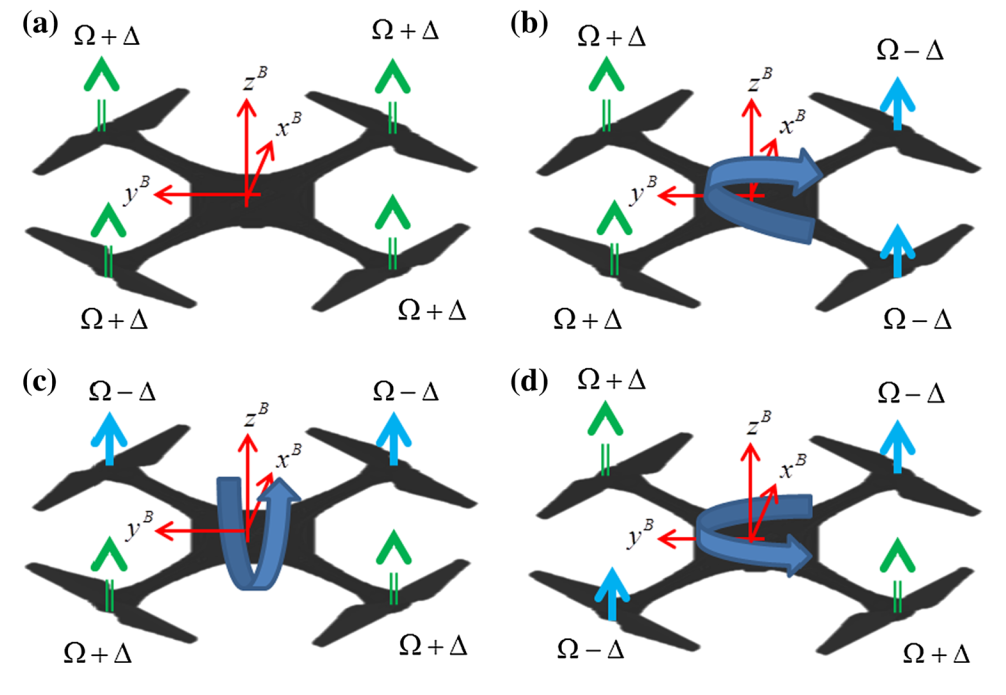
\includegraphics[scale=0.3]{partes/img/QUAV-modes.png}
    \caption[Modos de vuelo básicos de un QUAV.]{Modos de vuelo básicos de un QUAV \cite{multidrone2017review}. \textbf{(a)} Ascenso vertical, \textbf{(b)} \textit{Rolling}, \textbf{(c)} \textit{Pitching} y \textbf{(d)} \textit{Yawing}.} 
    \label{fig:QUAV-modes}
\end{figure}

\textit{Rolling} y \textit{Pitching} producen rotaciones sobre los ángulos \jim{\phi} y \jim{\theta} respectivamente, y producen una translación asociada en la dirección de los rotores que giran a menor velocidad \jim{\Omega - \Delta}. Efectivamente, \textit{Rolling} y \textit{Pitching} permiten mover al QUAV en la direcciones \jim{y_B} y \jim{x_B}. Por otro lado, \textit{Yawing} produce una rotación sobre el ángulo \jim{\psi} sin producir una translación asociada. \textit{Yawing} es importante porque es el modo de movimiento que modifica directamente el encabezamiento del QUAV.

\subsection{Localización GPS y coordenadas NED}

Tal como se menciona en la Sección \ref{sec:QUAV-sensors}, es habitual que un QUAV tenga acceso tanto a localización por visión como a localización por GPS, sin embargo, a efectos de este trabajo, se asume que el QUAV siempre utiliza localización por GPS. Para aplicaciones de evasion de obstáculos locales, utilizar directamente las coordenadas GPS puede resultar poco práctico debido a la diferencia de escalas. En concreto, la diferencia entre dos puntos cercanos en coordenadas GPS puede ser muy pequeña, lo que puede producir errores numéricos en el cálculo de la distancia entre dos puntos. Es por esto, que es importante establecer un sistema de coordenadas equivalente que no tenga este problema.

En el modelo geodésico del mundo WGS64, el que se utiliza en este trabajo, un punto en coordenadas GPS vienen dadas por la tupla latitud, longitud y altitud \jim{(\phi, \lambda, h)} \cite{2002convertGPS}. En la Figura \ref{fig:WGS64}, se muestra el elipsoide del modelo geodésico del mundo WGS64, donde se observa la coordenada \jim{(\phi, \lambda, h)} que representa el punto \jim{(x,y,z)}.

\begin{figure}[H]
    \centering
    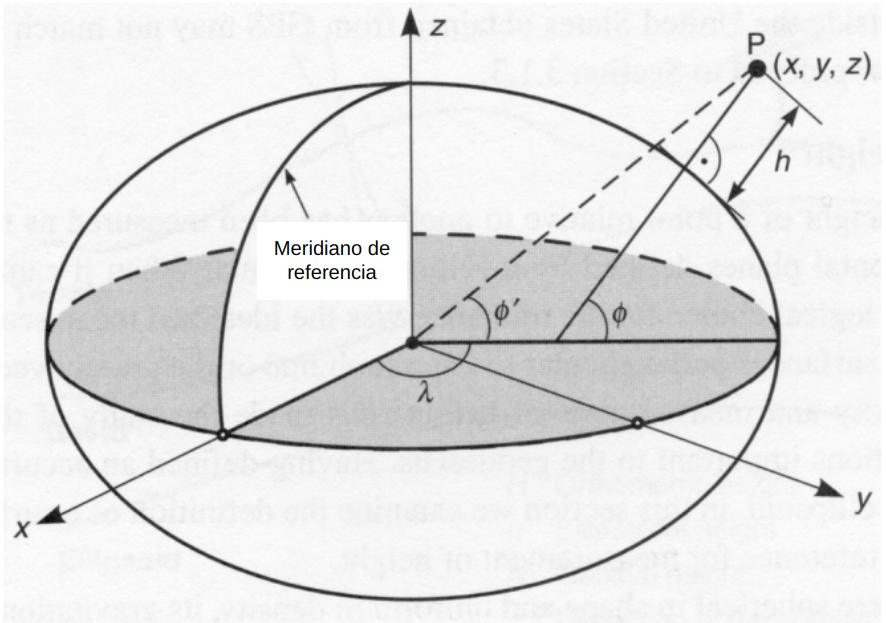
\includegraphics[scale=0.3]{partes/img/WGS64.png}
    \caption[Modelo geodésico del mundo WGS64.]{Modelo geodésico del mundo WGS64. Modificada de \cite{2002convertGPS}.} 
    \label{fig:WGS64}
\end{figure}

Dado \jim{S_{W}} el conjunto de puntos en la superficie del elipsoide WGS64. Un sistema de referencia sencillo de representar y que puede modelar los puntos \jim{(\phi, \lambda, h)} en el modelo WGS64, es el sistema de coordenadas NED (Norte, Este y Abajo; del inglés \textit{North, East, Down}) \cite{cai2011coordinate}. Este sistema es relativo a \jim{S_{W}} y sus puntos se representan con la tupla \jim{(n, e, d)} donde, dado un punto \jim{o = (\phi_0, \lambda_0) \in S_{W}}:

\begin{itemize}
    \item \jim{n} es el desplazamiento en metros hacia el \textbf{norte} del elipsoide a partir de \jim{o}.
    \item \jim{e} es el desplazamiento en metros hacia el \textbf{este} del elipsoide a partir de \jim{o}.
    \item \jim{h} es profundidad del punto en la \textbf{dirección normal} del elipsoide en \jim{o}.
\end{itemize}

El punto \jim{(\phi_0, \lambda_0, 0)} es el origen del sistema de coordenadas NED \cite{cai2011coordinate}, y suele definirse como el punto latitud, longitud de donde despega el QUAV \cite{multidrone2017review}.

Dada \jim{G: S_W \times S_W \longrightarrow \mathbb{R}^{+} \times \mathbb{R}^{+}} una función que recibe dos coordenadas \jim{a = (\phi_a, \lambda_a)} y \jim{b = (\phi_b, \lambda_b)} en \jim{S_W} y retorna el par real \jim{(\delta_n, \delta_e)} donde: 

\begin{itemize}
    \item \jim{\delta_n} es la longitud en metros del camino mas corto que va desde \jim{(\phi_a, \lambda_a)} hasta \jim{(\phi_b, \lambda_a)} sobre \jim{S_W}.
    \item \jim{\delta_e} es la longitud en metros del camino mas corto que va desde \jim{(\phi_a, \lambda_a)} hasta \jim{(\phi_a, \lambda_b)} sobre \jim{S_W}.
\end{itemize}

El Algoritmo \ref{alg:NED} muestra cómo transformar un punto \jim{(\phi, \lambda, h)} en WGS64 a NED.

\begin{algorithm}
\caption{Pseudo-código del algoritmo de transformación de coordenadas WGS64 a coordenadas NED}
\label{alg:NED}
\KwData{\jim{G}, \jim{(\phi, \lambda, h)}, \jim{(\phi_0, \lambda_0) \in S_{W}}}
\KwResult{\jim{(n, e, d)}}

$(\delta_n, \delta_e) = G((\phi_0, \lambda_0), (\phi, \lambda))$

$n = \text{sgn}(\phi - \phi_0) \cdot \delta_n$

$e = \text{sgn}(\lambda - \lambda_0) \cdot \delta_e$

$d = -h$;

\Return{\jim{(n, e, d)}}

\end{algorithm}


Donde \jim{\text{sgn}} es la función signo. \jim{G} usualmente es implementada utilizando la proyección de Mercator \cite{vis2018history} y existen una amplia selección de librerías de código abierto que la implementan.

\section{Visión estereoscópica}
\label{sec:teo-stereo}

El objetivo de los algoritmos de visión estereoscópica es obtener información tridimensional de una escena a partir de dos imágenes con distintas observaciones. Dado que la posición relativa entre las dos cámaras y los parámetros intrínsecos de cada una son conocidas, es posible obtener la información de profundidad de la escena utilizando relaciones geométricas entre las coordenadas tridimensionales y sus proyecciones en ambas imágenes \cite{sterovis}. Para que esto sea posible, es necesario que ambas imágenes estén rectificadas, esto es, que no tengan distorsión de lente y que se encuentren en el mismo plano; esto con el objetivo de que la diferencia entre una imagen y la otra sea un desplazamiento horizontal. La Figura \ref{fig:stereo-rectification} muestra un ejemplo del proceso de rectificación de un par de imágenes estéreo.

\begin{figure}[H]
    \centering
    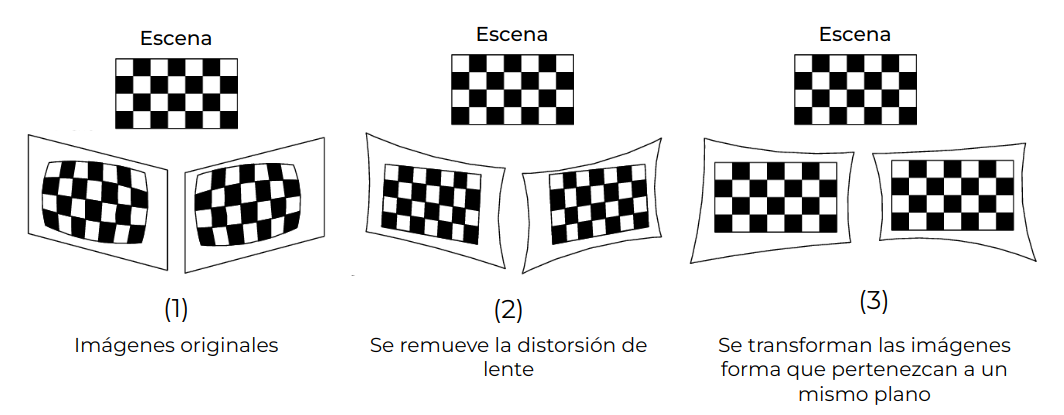
\includegraphics[scale=0.4]{partes/img/rectificacion.png}
    \caption[Ejemplo del proceso de rectificación de un par de imágenes estéreo.]{Ejemplo del proceso de rectificación de un par de imágenes estéreo. Modificada de \cite{Alberto2010}.}
    \label{fig:stereo-rectification}
\end{figure}

Con las imágenes rectificadas, el siguiente paso es obtener el desplazamiento horizontal entre las correspondencias píxel a píxel entre las dos imágenes, este desplazamiento se denomina disparidad. El arreglo bidimensional de la disparidad píxel a píxel entre dos imágenes estéreo se denomina mapa de disparidad, los mapas de disparidad nos permiten representar la información de la disparidad de todos los píxeles de una manera más accesible, ya que se puede interpretar como un imagen, tal como se muestra en la Figura \ref{fig:stereo-diparity-map}.

\begin{figure}[H]
    \centering
    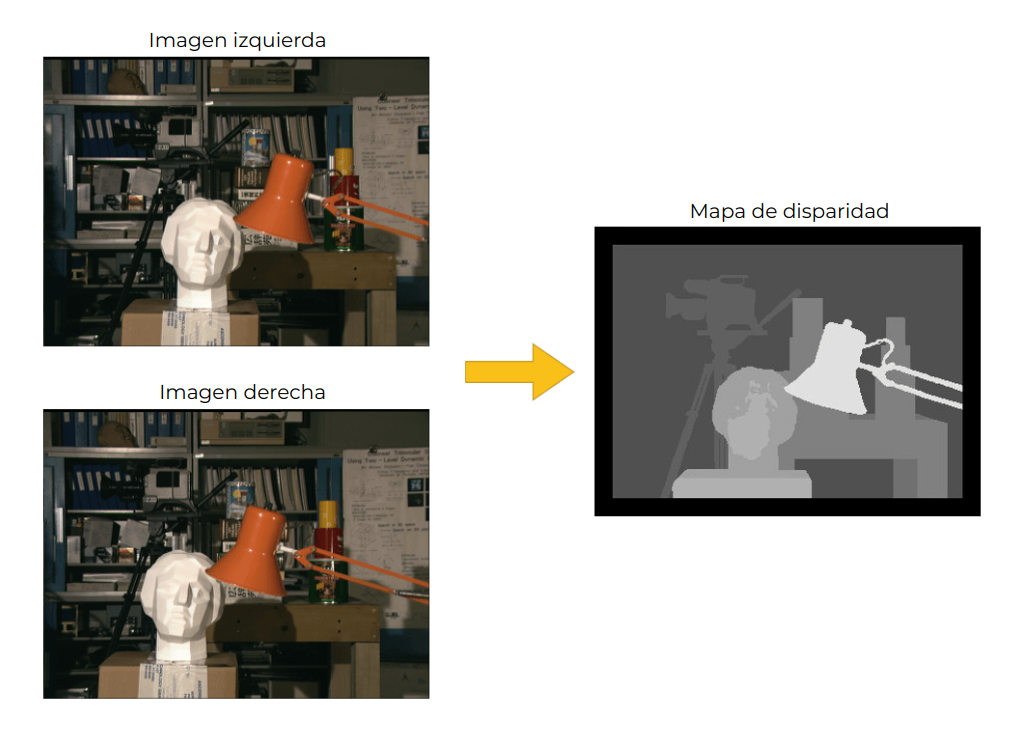
\includegraphics[scale=0.4]{partes/img/disparity-map.png}
    \caption[Ejemplo de la representación de un mapa de disparidad como una imagen.]{Ejemplo de la representación de un mapa de disparidad como una imagen\footnotemark.} 
    \label{fig:stereo-diparity-map}
\end{figure}
\footnotetext{Modificada de: \url{https://www.baeldung.com/cs/disparity-map-stereo-vision}}

Para calcular un mapa de disparidad hace falta establecer correspondencias píxel a píxel entre el par de imágenes estéreo. Un método para establecer estas correspondencias es el Emparejamiento de Bloques \cite{Baudes2009} (BM, del inglés \textit{Block Matching}). El BM consiste en obtener correspondencias entre imágenes estéreo rectificadas, tomando bloques de píxeles en la primera imagen y buscando los bloques mas similares en la segunda imagen; la búsqueda se realiza desplazando el dominio del bloque únicamente de forma horizontal a partir de la misma fila del bloque de la primera imagen; el criterio de búsqueda involucra una función de desemejanza entre bloques de píxeles, usualmente la Suma de Diferencias Absolutas (SAD, del inglés \textit{Sum of Absolute Differences}), y se seleccionan dos bloques como correspondientes si el valor de la función de desemejanza es mínimo local a lo largo de los posibles desplazamientos a partir de la posición inicial del bloque. En la Figura \ref{fig:stereo-block-matching} se ilustra un ejemplo de la correspondencia establecida por BM, y se observa el valor de la función de desemejanza en función de los desplazamientos (disparidad), el bloque seleccionado es aquel cuyo valor de la función de desemejanza sea mínimo local. BM permite obtener un valor de disparidad para cada píxel; finalmente, con este resultado se puede construir un mapa de disparidad.

\begin{figure}[H]
    \centering
    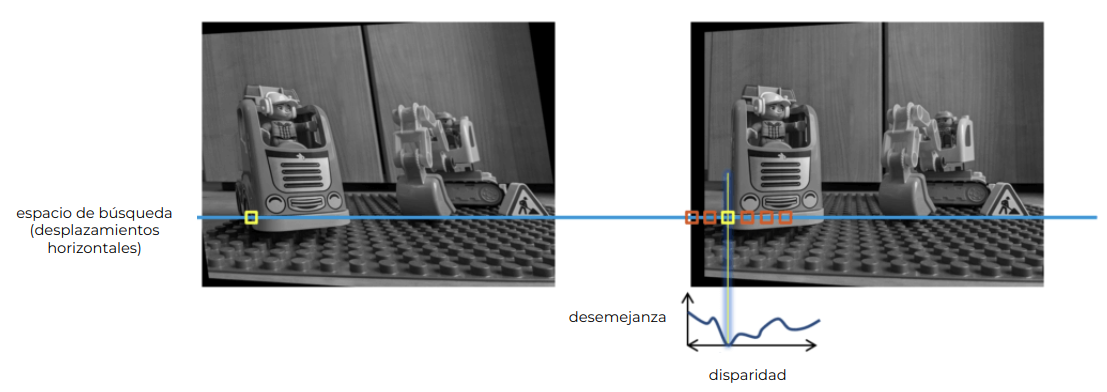
\includegraphics[scale=0.4]{partes/img/block-matching.png}
    \caption[Ejemplo del Emparejamiento de Bloques para establecer correspondencias entre un par de imágenes estéreo rectificadas.]{Ejemplo del Emparejamiento de Bloques para establecer correspondencias entre un par de imágenes estéreo rectificadas\footnotemark.} 
    \label{fig:stereo-block-matching}
\end{figure}
\footnotetext{Modificada de: \url{https://www.andreasjakl.com/understand-and-apply-stereo-rectification-for-depth-maps-part-2/}}

Una vez que se que se tiene el mapa de disparidad, es posible obtener la información de profundidad tridimensional de cada píxel utilizando relaciones geométricas, en particular, triangulación. En la Figura \ref{fig:stereo-triang} se muestra el modelo de un sistema de visión estereoscópica de dos cámaras paralelas \jim{C} y \jim{C^{\prime}}. En esta se observa: la distancia \jim{b}, que es la distancia entre las cámaras; la distancia \jim{f}, que es la distancia focal, es decir, la distancia entre el lente y el sensor; y un punto 3D en la escena, que corresponde al par de correspondencia píxel píxel \jim{u}, \jim{u^{\prime}} con disparidad \jim{d = (u_x - u^{\prime}_x)}. Los valores de \jim{b} y \jim{f} son determinados por el tipo y configuración de las cámaras, y se calculan mediante un proceso de calibración. Una vez conocidos, la profundidad \jim{D} del punto 3D en la escena con respecto al par estéreo se calcula utilizando la Ecuación \ref{eq:stereo-depth}. 

\begin{figure}[H]
    \centering
    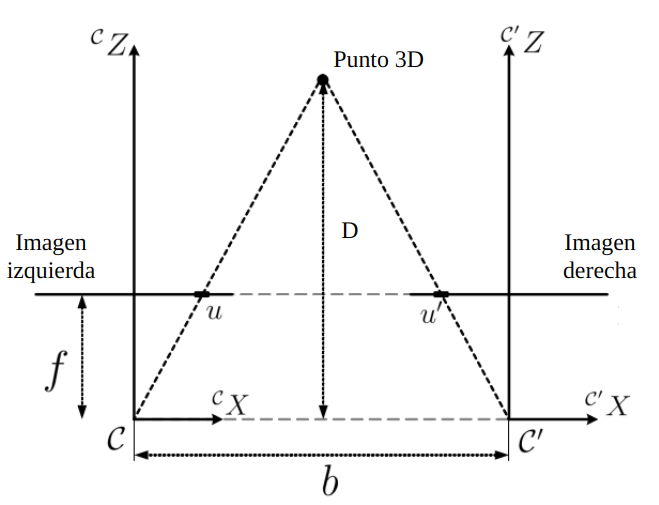
\includegraphics[scale=0.4]{partes/img/stereo-trangulation.png}
    \caption[Modelo de un sistema de visión estereoscópica de dos cámaras paralelas \jim{C} y \jim{C^{\prime}}.]{Modelo de un sistema de visión estereoscópica de dos cámaras paralelas \jim{C} y \jim{C^{\prime}}. Modificada de \cite{Alberto2010}.}
    \label{fig:stereo-triang}
\end{figure}

\begin{equation}
    \label{eq:stereo-depth}
    D =  \frac{f \cdot b}{u_x - u^{\prime}_x} = \frac{f \cdot b}{d}
\end{equation}

Si se calcula la profundidad \jim{D} para cada correspondencia representada en el mapa de disparidad se obtiene un mapa de profundidad que codifica la información tridimensional de la escena, dicho mapa de profundidad también se puede interpretar en una imagen de manera análoga a lo que se observa en la Figura \ref{fig:stereo-diparity-map}.

\section{Redes neuronales}
\label{sec:teo-neural}

Una red neuronal es un modelo matemático que trata de imitar el funcionamiento del cerebro humano para resolver problemas o tareas, donde las unidades básicas son las neuronas. Cada neurona recibe datos de entrada, realiza cálculos con ellos y produce una salida. La salida de una neurona se convierte en la entrada de otras neuronas, creando así una red de procesamiento. Tal como sus equivalentes biológicos, las redes neuronales son capaces de representar aprendizaje, así como adaptarse a través de la experiencia. Durante un proceso denominado entrenamiento, estas redes ajustan las conexiones entre sus neuronas, fortaleciendo o debilitando ciertas conexiones en función de la retroalimentación proporcionada por los datos observados. A medida que la red es expuesta a un mayor número de ejemplos y recibe retroalimentación constante, su capacidad para reconocer patrones, tomar decisiones o resolver problemas en esa tarea se fortalece.

Matemáticamente, una red neuronal es una serie de nodos interconectados, cada nodo recibe entradas de otros nodos y su respuesta se utiliza de entrada para otros nodos. Cada conexión tiene asociada un peso, que es un número real; cada nodo multiplica sus entradas con el respectivo peso de la conexión, suma los productos y le aplica una función de activación \cite{Gurney1997}; la función de activación es una función matemática simple que modela el proceso de disparo o activación de una neurona biológica. La Figura \ref{fig:nn-single-node} ilustra el funcionamiento de un nodo dentro de una red neuronal.

\begin{figure}[H]
    \centering
    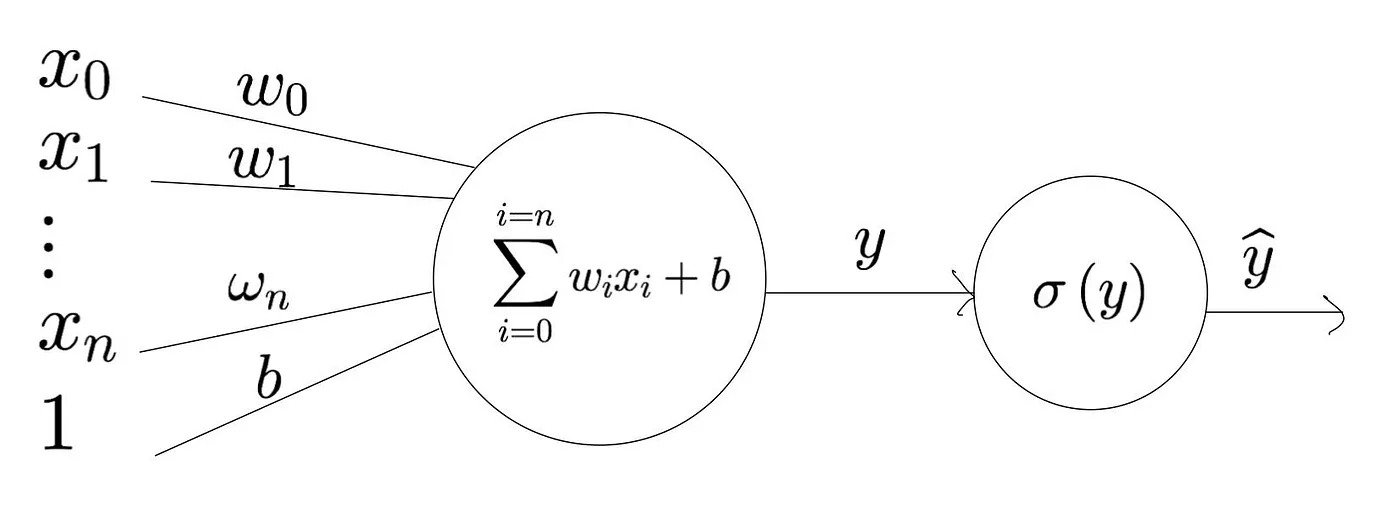
\includegraphics[scale=0.25]{partes/img/perceptron.jpg}
    \caption[Funcionamiento de un nodo de una red neuronal.]{
        Funcionamiento de un nodo de una red neuronal\footnotemark. \jim{n} es el número entradas del nodo. \jim{x_i} son las entradas del nodo y \jim{w_i} son los pesos asociados a sus conexiones, con \jim{0 \leq i \leq n}. Luego, \jim{\sigma} es la función de activación y \jim{b} es un peso asociado a una entrada constante, usualmente es llamado sesgo.
    } 
    \label{fig:nn-single-node}
\end{figure}
\footnotetext{Obtenida de: \url{https://medium.com/analytics-vidhya/perceptron-learning-from-discrete-to-continuous-02-b16ddf9e5ab6}}

La motivación matemática de la función de activación es introducir no linealidad a la salida del nodo, para ello existen una gama de funciones de activación ampliamente utilizadas, entre estas de encuentran: la función tangente hiperbólica, la función sigmoide y las Unidades Lineales Rectificadas (ReLU, del inglés \textit{Rectified Linear Units}), la Ecuación \ref{eq:tanh}, la Ecuación \ref{eq:sigmoid} y la Ecuación \ref{eq:relu} respectivamente muestran las definiciones de las funciones mencionadas anteriormente.

\begin{equation}
    \label{eq:tanh}
    \tanh(x) = \frac{\sinh(x)}{\cosh(x)} = \frac{e^x - e^{-x}}{e^x + e^{-x}}
\end{equation}

\begin{equation}
    \label{eq:sigmoid}
    \sigma(x) = \frac{1}{1 + e^{-x}}
\end{equation}

\begin{equation}
    \label{eq:relu}
    \mathrm{ReLU}(x)= \begin{cases} 
        0 & \text { si } x<0 \\
        x & \text { si } x \geq 0
    \end{cases}
\end{equation}

Las redes neuronales se pueden estructurar por capas, cada capa tiene una serie de nodos que reciben sus entradas de todos los nodos de la capa anterior y a su vez sirven de entrada todos los nodos de la capa superior; no existen conexiones entre nodos que pertenezcan a una misma capa y no existen capas que reciban como entrada a los nodos de alguna capa superior. Cuando una red neuronal se estructura por capas de la forma descrita anteriormente se le denomina Red Neuronal de Alimentación hacia adelante \cite{huang2019deep}, FFNN del inglés \textit{Feed-forward Neural Network}. 

\begin{figure}[H]
    \centering
    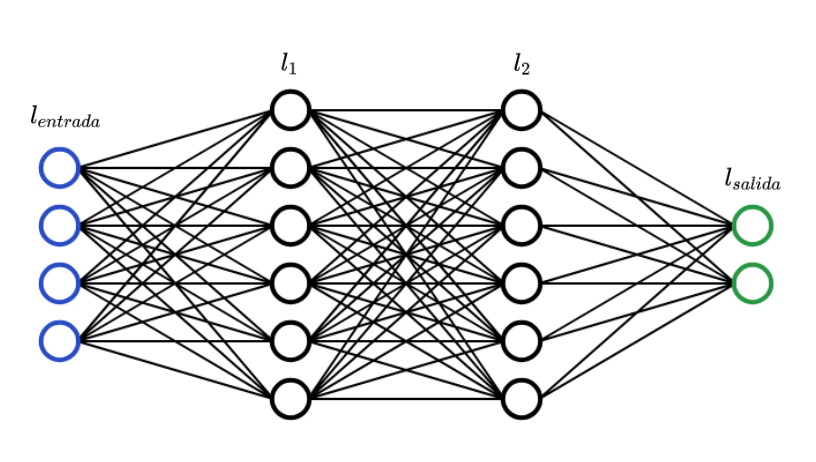
\includegraphics[scale=0.4]{partes/img/nn-capas.png}
    \caption[Ejemplo de una FFNN con dos capas ocultas.]{
        Ejemplo de una FFNN con dos capas ocultas\footnotemark. \jim{l_{entrada}} y \jim{l_{salida}} son las capas de entrada y de salida respectivamente. \jim{l_1} y \jim{l_2} son las capas ocultas, también llamadas capas completamente conectadas, FC del inglés \textit{Fully Connected}.
    } 
    \label{fig:nn-layers}
\end{figure}
\footnotetext{Modificada de: \url{https://victorzhou.com/series/neural-networks-from-scratch/}}


Un ejemplo de una FFNN de muestra en la Figura \ref{fig:nn-layers}. Las FFNN tienen una capa de entrada y una de salida (\jim{l_{entrada}} y \jim{l_{salida}} en la Figura \ref{fig:nn-layers}), la capa de entrada recibe el estimulo inicial de la red, mientras que la capa de salida retorna la respuesta de la red al estímulo. Además, las FFNN se caracterizan por el número de capas FC (\jim{l_1} y \jim{l_2} en la Figura \ref{fig:nn-layers}), mientras más capas ocultas, se dice que la red es más ``profunda". El conjunto de los pesos de los nodos de una red se denomina \jim{\theta}, mientras que un peso en particular se denomina \jim{w_{j}} donde \jim{j} es el índice de la transición asociada al peso. Al modificar pesos \jim{\theta} se modifica el comportamiento de la red ante un estimulo; diferentes combinaciones de valores de \jim{\theta} producen comportamientos distintos; así, la representación del ``conocimiento" de una red neuronal se encuentra almacenado en sus pesos \jim{\theta}. Mediante algoritmos de aprendizaje automático se pueden modificar sistemáticamente los pesos de la red neuronal para que se adapte a una tarea en especifica, este proceso de adaptación también es denominado entrenamiento \cite{Gurney1997}.

\subsection{Retro-propagación}

El algoritmo de retro-propagación (del inglés \textit{backpropagation}) es un algoritmo de aprendizaje supervisado que se utiliza para entrenar redes neuronales. Este algoritmo ajusta los pesos de las conexiones entre los nodos de la red neuronal de manera que la red pueda realizar una tarea en específico (clasificación o regresión por ejemplo). El algoritmo de retro-propagación utiliza el denominado descenso de gradiente (del inglés \textit{Gradient Descent}), el cual es un método utilizado para minimizar una función de pérdida que cuantifica el error entre las predicciones de la red y los valores objetivos asociados a la tarea seleccionada.

\subsubsection{Descenso de gradiente}

El aprendizaje automático supervisado presenta iterativamente un conjunto de patrones de entrada (\jim{X}) y de salida (\jim{Y}) al modelo, en este caso una red neuronal. En cada iteración se modifican los pesos \jim{\theta} de acuerdo a una regla de actualización cuyo objetivo es que la salida de la red se asemeje a la salida deseada \cite{Gurney1997}. Para realizar estos cambios, la regla de actualización debe cuantificar que tan bien la red neuronal modela los datos que se le presentan; es por esto que se define una función de costo o error \textit{E} que dado un dado de entrada \jim{x_k}, el vector deseado \jim{y_k} y los pesos \jim{\theta} de la red, retorna \jim{E(x_k, y_k, \theta)} que cuantifica que tan similar a \jim{y_k} es la salida de la red (parametrizada por \jim{\theta}) cuando se le pasa como entrada \jim{x_k}. El objetivo es que la red sea capaz de modelar la relación entre los patrones de entrada \jim{X} y salida \jim{Y}, en otras palabras, se quiere minimizar la función descrita en la Ecuación \ref{eq:loss}; esta función se denomina función de pérdida, donde \jim{|X| = |Y|} y \jim{x_k, y_k} son el patrón entrada salida número \jim{k} con \jim{x_k \in X \wedge y_k \in Y}. Finalmente el problema de minimización tratado en este trabajo es el descrito en la Ecuación \ref{eq:optim-problem}.

\begin{equation}
    \label{eq:loss}
    L(X, Y, \theta) = \sum_{k = 1}^{|X|} E(x_k, y_k, \theta)
\end{equation}

\begin{equation}
    \label{eq:optim-problem}
    \min_{\theta} L(X, Y, \theta)
\end{equation}

Tal como su nombre lo indica, el descenso de gradiente en cada iteración se mueve en la dirección del gradiente, esto lo hace siguiendo la regla de actualización:

\begin{equation}
    \label{eq:gd-update-rule}
    \theta = \theta - \alpha \nabla_{\theta} L(X, Y, \theta)
\end{equation}

Donde \jim{0 < \alpha < 1} es un número real llamado "tasa de aprendizaje"; \jim{\alpha} se encarga de que la regla de actualización no produzca cambios drásticos que puedan dificultar la convergencia del algoritmo. Luego, la regla de actualización de cada peso individual \jim{w_{j}} viene dada por:

\begin{equation}
    \label{eq:gd-update-rule-item}
    w_{j} = w_{j} - \alpha \frac{\partial L(X, Y, \theta)}{\partial w_{j}}
\end{equation}

Estas regla de actualización se aplica iterativamente sobre el conjunto de patrones entrada salida (también llamado conjunto de entrenamiento) hasta alcanzar un criterio de convergencia, como un valor umbral de la función de pérdida o un número de iteraciones. Justamente esta es la descripción del algoritmo del descenso de gradiente.

Dado un conjunto de datos de entrada \jim{X}, un conjunto de valores deseados \jim{Y}, la tasa de aprendizaje \jim{\alpha} y una función booleana \jim{Q(\theta)} que sirve como criterio de convergencia. El Algoritmo \ref{alg:dg} muestra el pseudo-código del proceso de retro-propagación usando descenso de gradiente.

\begin{algorithm}
\caption{Pseudo-código del algoritmo de retro-propagación usando descenso de gradiente}
\label{alg:dg}
\KwData{\jim{X, Y, \alpha, Q}}
\KwResult{\jim{\theta}}

Inicializar los pesos \jim{\theta} en ceros o en valores aleatorios cercanos a cero

\While{\jim{\neg Q(\theta)}}{
    \For{\jim{w_j \in \theta}}{
        \jim{w_{j} = w_{j} - \alpha \frac{\partial L(X, Y, \theta)}{\partial w_{j}}}
    }
}
\end{algorithm}

\subsubsection{Sub-ajuste y sobre-ajuste}

La arquitectura de una red neuronal (número de capas y de nodos por capa) y el criterio de convergencia del descenso de gradiente deben elegirse cuidadosamente para evitar sesgos que puedan afectar negativamente el rendimiento del modelo. Hay dos tipos de errores a los que puede conducir un sesgo inapropiado: sub-ajuste y sobre-ajuste. El sub-ajuste (del inglés \textit{underfitting}) ocurre cuando la arquitectura de la red es demasiado simple para representar la relación entre los datos de entrada y los valores deseados del conjunto de entrenamiento, o cuando el criterio de convergencia es demasiado temprano. Por otro lado, el sobre-ajuste (del inglés \textit{overfitting}) ocurre cuando la arquitectura de la red es muy compleja o se realizan demasiadas iteraciones del descenso de gradiente, lo que hace que el modelo se ajuste demasiado al conjunto de datos de entrenamiento. Los modelos con sub-ajuste o sobre-ajuste no generalizan correctamente y, por lo tanto, no sera buenos al momento de realizar inferencia sobre datos que estén más allá de lo que se observó durante el entrenamiento.

\subsection{Redes neuronales convolucionales}

Cuando se desea utilizar una imagen como entrada de una red neuronal, cada píxel de la imagen es una entrada de la red; considerando que incluso imágenes de resoluciones relativamente bajas contienen un número de píxeles en el orden de los miles y hasta tres canales de color, si se utilizara una red con solo capas FC, la cantidad de pesos a entrenar seria muy elevada debido a la alta cantidad de entradas; una imagen a color de 300 píxeles de ancho por 300 de alto necesitaría \jim{300 \cdot 300 \cdot 3 = 270000} nodos de entrada, colocando el número de pesos de la red en el orden los cien miles con tan solo una capa, por esto el uso de redes neuronales con solo capas FC no es conveniente para trabajar con imágenes.

Las redes neuronales convolucionales (CNN, del inglés \textit{Convolutional Neural Networks}) son un tipo de red neuronal FFNN, principalmente utilizadas para el procesamiento digital de imágenes, que debido a su estructura permiten reducir la cantidad de pesos necesarios a entrenar; habilitando un proceso de entrenamiento más sencillo y a mayor velocidad \cite{Lecun2010}. Las CNN incorporan tres tipos de capas: las capas convolucionales, las capas de submuestreo (del inglés \textit{pooling layers}) y capas FC generalmente al final de la red.

Las CNN suelen componerse de dos partes: un denominado extractor de características, conformado por capas convolucionales y capas de submuestreo; y parte FC cuyo objetivo varia dependiendo de la tarea que se requiere de la red (regresión o clasificación por ejemplo). En la Figura \ref{fig:cnn-sample} se muestra un ejemplo de la arquitectura de una CNN.

\begin{figure}[H]
    \centering
    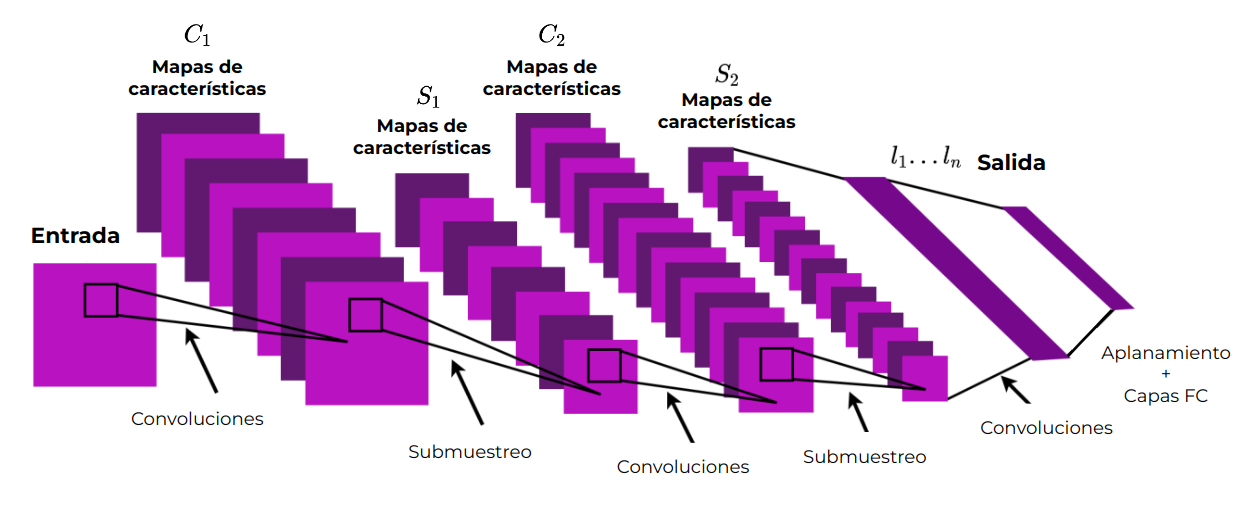
\includegraphics[scale=0.35]{partes/img/CNN-sample.png}
    \caption[Ejemplo de la arquitectura de una CNN.]{
        Ejemplo de la arquitectura de una CNN \cite{Lecun2010}. \jim{C_1} y \jim{C_2} son los resultados de capas convolucionales, \jim{S_1} y \jim{S_2} son los resultados de capas de submuestreo. \jim{l_1 ... l_n} son \jim{n} capas FC. Entre \jim{S_2} y \jim{l_1} se realiza un proceso de aplanamiento, que concatena los mapas de características de \jim{S_2} para producir un vector de características que sirve de entrada para \jim{l_1}.
    } 
    \label{fig:cnn-sample}
\end{figure}

La intuición detrás de las capas convolucionales es la de la aplicación de filtros en espacio sobre imágenes para la extracción de mapas que codifican información de la entrada \cite{Gupta2013} \cite{Coady2019}. Las capas convolucionales realizan operaciones de convolución discreta a la matriz (imagen) de entrada, utilizando filtros también llamados \textit{kernels}. El resultado de una capa convolucional es una matriz en donde cada componente corresponde a la multiplicar uno de los \textit{kernels} con una región de la imagen de entrada, sumar los resultados y opcionalmente aplicar una función de activación. Estas capas de usan para la detección de características, es por eso que a la salida de estas capas se le da el nombre de ``mapa de características". El ancho y el alto de este mapa dependen de las dimensiones del \textit{kernel}, mientras que su número de canales es igual al número de \textit{kernels} utilizados por la capa.

Las capas de submuestreo se tienen la finalidad de filtrar características poco relevantes de la entrada, su salida es un mapa de características donde cada componente es el resultado de una operación de reducción de dimensionalidad de una región del mapa de entrada. La operación de reducción de dimensionalidad usualmente es de uno de los siguientes tipos: promedio de la región seleccionada, en cuyo caso se le llama submuestreo por promedio (del inglés \textit{average pooling}); o máximo de la región seleccionada, llamando entonces submuestreo por máximo (del inglés \textit{max pooling}). El efecto de reducción de dimensionalidad ayuda a reducir el número de operaciones convolucionales de capas posteriores, haciendo el proceso de entrenamiento mas sencillo y veloz.

Entre el extractor de características y la parte FC se hace un proceso de aplanamiento (del inglés \textit{flattening}), cuyo resultado es la concatenación de los mapas de características para producir un vector de características que sirve de entrada para las capas FC de la red. La sección FC recibe el vector de características y genera una salida cuyas dimensiones dependen de la tarea en la cual se esta entrenando la red, estas capas FC siguen la misma estructura descrita en la Sección \ref{sec:teo-neural}.

\section{Comunicación entre procesos}
\label{sec:teo-interprocess}

La comunicación entre procesos, comúnmente abreviada como IPC (por sus siglas en inglés, Inter-Process Communication), se refiere al conjunto de técnicas y mecanismos utilizados para permitir que diferentes procesos intercambien información entre sí de forma asíncrona. Esta comunicación es fundamental en escenarios donde varias aplicaciones deben colaborar para lograr una funcionalidad más amplia. A través de IPC, los procesos pueden compartir datos, sincronizar su ejecución, coordinar tareas y garantizar la seguridad y eficiencia en la gestión de recursos compartidos. Algunos de los métodos de IPC utilizados comúnmente son las tuberías (del inglés \textit{pipes}), los \textit{sockets} y la memoria compartida \cite{IPCEval2015}.

\subsection{Tuberías}

Una tubería o \textit{pipe} es un método de comunicación unidireccional que permite la transferencia serial de información desde el proceso escritor al proceso lector. La capacidad de transferencia de datos de un tubería esta limitada por un búfer de tipo primero que entra, primero que sale (FIFO, del inglés \textit{First In, First Out}); cuando el escritor envía datos estos se agregan al búfer, de forma análoga cuando el lector procesa datos estos se eliminan del búfer; si el escritor escribe más rápido de lo que el lector consume datos y si el búfer de la tubería está lleno, el escritor se bloqueará hasta que haya más capacidad disponible. De manera similar, si el lector lee cuando la tubería está vacía, el lector se bloqueará \cite{IPCEval2015}. Con una tubería se pueden implementar esquemas de comunicación de mayor nivel de tipo productor-procesador (Pub/Sub, del inglés \textit{Publisher/Subscriber}) siempre y cuando solo exista solo un productor y solo un procesador.

\subsection{\textit{Sockets}}

Un \textit{socket} es un mecanismo de comunicación bidireccional que se puede utilizar para comunicar un proceso con otro proceso, bien sea dentro de la misma máquina o en una máquina diferente \cite{IPCEval2015}. Los datos enviados a través de un \textit{socket} se dividen en fragmentos llamados paquetes. Un protocolo, como TCP/IP, especifica cómo se transmiten estos paquetes a través del \textit{socket}. Un \textit{socket} se identifica de manera única mediante una combinación de la dirección IP de la máquina y un número de puerto. La bidireccionalidad de los \textit{sockets} permite construir esquemas de comunicación a alto nivel sin restricciones de cardinalidad (tales como Pub/Sub con muchos productores y muchos receptores), si bien la implementación de estos esquemas puede ser complicado,  existen múltiples librerías de implementaciones estables de estos, tales como ZeroMQ \cite{zeroMQ}.

\subsection{Memoria compartida}

La memoria compartida permite a dos o más procesos acceder al mismo espacio de memoria, este espacio es mapeado al espacio de direcciones de memoria de cada uno de los procesos participantes \cite{IPCEval2015}. Dado que esta comunicación es similar a cualquier otra referencia de memoria, no implica ninguna llamada al sistema ni latencias inducidas por protocolos. Por lo tanto, generalmente la memoria compartida ofrece latencias muy bajas. Sin embargo, el sistema no proporciona ningún mecanismo sincronización implícito para los accesos a la memoria compartida; esto significa que el uso descuidado de la memoria compartida puede producir condiciones de carrera \cite{IPCEval2015}. El uso de mecanismos de primitivas como los semáforos o los \textit{mutex} pueden habilitar el uso de la memoria compartida sin riesgo de inconsistencia en los datos, pero su implementación es responsabilidad del programador.

\section{Resumen}

En este capítulo se establecen las bases teóricas necesarias para el desarrollo del trabajo, incluyendo el modelado de vehículos aéreos no tripulados de cuatro rotores y el procedimiento para la obtención de mapas de profundidad a partir de un sistema de cámaras estereoscópicas. Adicionalmente, se explican los fundamentos de las redes neuronales, su proceso de entrenamiento y sus variantes enfocadas al procesamiento de imágenes, las CNN. Finalmente, se describieron algunos métodos de comunicación entre procesos que nos serán útiles durante el desarrollo del presente trabajo.

En el siguiente capítulo, se hace una revisión del estado del arte de los métodos de evasión de obstáculos para drones y se profundiza en \textit{Learning high-speed flight in the wild}, un método bastante atractivo para el desarrollo de este trabajo en el contexto de la plataforma disponible para su implementación.
\chapter{Antecedentes}
\label{capitulo4}
\lhead{Capítulo 4. \emph{Estado del Arte}}


El problema de evasión de obstáculos es un problema de planificación local de caminos. Entre las investigaciones que abordan este problema, existen dos variantes, las que dependen de la información global disponible previamente al momento de la planificación del camino, y aquellos desarrollos que presentan soluciones que dependen únicamente de la información de los sensores disponibles a bordo del vehículo, al momento de la planificación del camino. En este capitulo se hace una revisión del estado del arte de ambas variantes mencionadas anteriormente, explorando la primera variante en la sección \ref{sec::prev-global}, la segunda variante en la sección \ref{sec::prev-local}, y profundizando en \textit{Learning high-speed flight in the wild} en la sección \ref{sec::prev-agile-autonomy}, que es el principal antecedente del desarrollo del presente trabajo.

\section{Desarrollos que dependen de la información global del entorno}
\label{sec::prev-global}

Este tipo de investigaciones separan sus algoritmos en dos etapas, una etapa fuera de línea (del inglés \textit{offline}) que se ejecuta antes de que el UAV comience el vuelo, y una etapa en línea (del inglés \textit{online}) que se ejecuta durante la ejecución del vuelo. La etapa fuera de línea considera la información global del entorno, esto es, modelos del entorno, que pueden expresados por grafos, nube de puntos, entre otros; información del estado del entorno, que describen los eventos que ocurren en el entorno en el tiempo, como listas de vuelos consecutivos o posición de obstáculos programados en función del tiempo. La etapa en línea depende de los artefactos generados por la etapa fuera de línea y generalmente permiten que la complejidad de ejecución de la etapa en línea sea ligera. Sin embargo, la dependencia de la etapa fuera de línea en la información global del entorno, hace que este tipo de soluciones no sean viables en aplicaciones donde se desconoce a priori la información global del entorno. A continuación se describen brevemente algunas investigaciones que proponen este tipo de métodos.

En \cite{shi2018collision} se propone un método que genera en la etapa fuera de línea un camino libre de colisiones utilizando un algoritmo basado en A* que considera el grafo del espacio aéreo del entorno, una lista de sectores restringidos por situaciones climáticas o de regulaciones y la lista de los caminos en ejecución de otros UAV. Los caminos producidos por este algoritmo evitan obstáculos estáticos (en forma de sectores restringidos), así como también obstáculos dinámicos (en forma de caminos en ejecución). Este método tiene la ventaja de que si se mantiene correctamente la lista de caminos en ejecución, es posible orquestar la navegación de múltiples UAV en el entorno sin producir colisiones con obstáculos. Este tipo de métodos basados en A* tienen la desventaja de su etapa en línea no posee la capacidad de adaptarse a obstáculos no previstos en la etapa fuera de linea, en otras palabras, el camino se vuele completamente estático una vez que el UAV comienza el vuelo \cite{park2020boundary}; sin mencionar que su funcionamiento depende de que exista un grafo que modele el entorno correctamente.

Otros métodos tales como los presentados en \cite{lifen2016path} utilizan campos potenciales artificiales para planificar caminos libres de colisión. La planificación de caminos por campos potenciales artificiales conciben al vehículo como una partícula inmersa en un campo de potencial cuyas variaciones locales reflejan la estructura del entorno \cite{bermudez2004aplicacion}, donde potenciales atractivos representan posiciones objetivo y potenciales repulsivos representan obstáculos, luego la trayectoria del vehículo es determinada iterativamente siguiendo el sentido de la fuerza producida por el potencial. En \cite{lifen2016path} se utiliza este concepto para producir caminos libres de colisión para la navegación de un UAV dentro de un entorno donde la ubicación de los obstáculos es conocida antes de comenzar el vuelo. La etapa fuera de línea en \cite{lifen2016path} calcula el camino a ejecutar siguiendo el potencial establecido por la información del entorno (obstáculos y posiciones objetivo) y la etapa en línea ejecuta este camino. Si bien \cite{lifen2016path} no lo hace, es posible que la etapa en línea recalcule localmente el camino inicial dado que se haya detectado algún obstáculo no previsto, sin embargo, esto introduce latencia en el sistema que pueden afectar la autonomía del vuelo. Este tipo de métodos basados en campos potenciales artificiales tienen la desventaja de que pueden hacer que el vehículo alcance mínimos locales de potencial que no permiten que el vehículo alcance su objetivo. Adicionalmente, estos métodos también son propensos a producir oscilaciones en la trayectoria, lo hace que la navegación no sea óptima y se desperdicie tiempo de vuelo, que justamente es uno de los recursos mas importantes para los UAV.


Por otro lado, en \cite{Zhang2019} se introduce P-CAL (Canales Alternativos Pre-calculados, del inglés \textit{Pre-computed Alternative Lanes}). Este método, en la etapa fuera de linea, dado un nube de puntos previamente calculada que codifica la información tridimensional del entorno, genera una colección de distintos caminos libres de colisión alternativos denominados canales (del inglés \textit{lanes}); entre cada canal adicionalmente se genera un camino de transición que permite cambiar de canal de forma fluida. Luego, en la etapa en linea, se alterna entre los distintos canales dependiendo de la presciencia de obstáculos no previstos. En otras palabras, P-CAL calcula un conjunto de caminos alternativos y luego alterna entre estos para evitar obstáculos imprevistos en el entorno. La detección de los obstáculos no previstos se hace comparando la información tridimensional predefinida del entorno con la lectura sensorial de un sensor LiDAR. La figura \ref{fig:P-CAL} muestra la nube de puntos del entorno previamente calculada, el resultado de la generación de los canales y caminos de transición; y el camino resultante de alternar canales para evadir obstáculos no previstos. El requerimiento de poseer una nube de puntos del entorno previo al vuelo del UAV, así como también la necesidad de utilizar un LiDAR para detectar obstáculos no previstos, hacen que este método no sea práctico para aplicaciones generales de evasión de obstáculos en donde no se tiene información previa del entorno o aquellas cuyos UAV no tengan la capacidad de utilizar un sensor LiDAR. 

\begin{figure}
    \centering
    \begin{subfigure}[b]{0.7\textwidth}
        \centering
        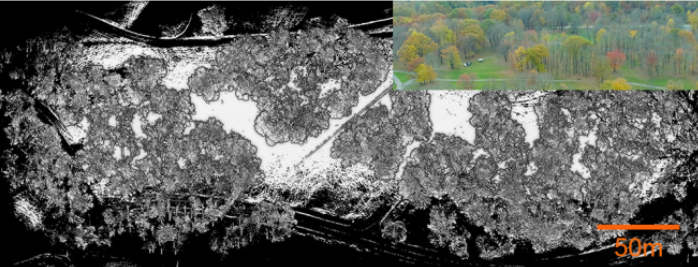
\includegraphics[width=\textwidth]{partes/img/P-CAL-map.png}
        \caption{Nube de puntos del entorno.}
    \end{subfigure}
    \hfill
    \begin{subfigure}[b]{0.7\textwidth}
        \centering
        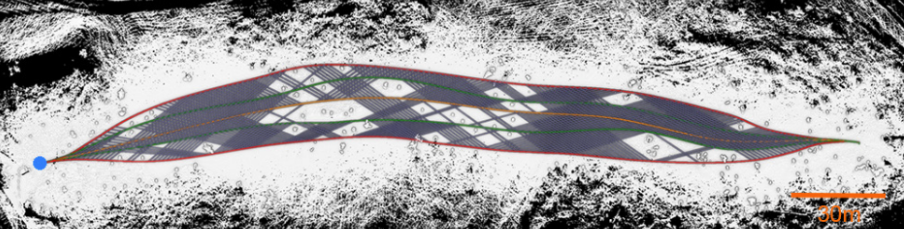
\includegraphics[width=\textwidth]{partes/img/P-CAL-lanes.png}
        \caption{Canales y caminos de transición.}
    \end{subfigure}
    \break
    \begin{subfigure}[b]{0.5\textwidth}
        \centering
        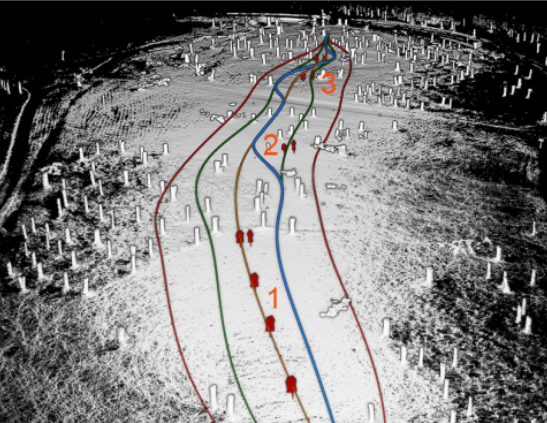
\includegraphics[width=\textwidth]{partes/img/P-CAL-results.png}
        \caption{Camino resultante.}
    \end{subfigure}
    \hfill
    
    \caption [P-CAL: Canales Alternativos Pre-calculados]{P-CAL, Canales Alternativos Pre-calculados \cite{Zhang2019}. \textbf{(a)} Nube de puntos del entorno previamente calculada. \textbf{(b)} Canales (amarillo, verde y rojo) y caminos de transición (azul) generados en la etapa fuera de linea. \textbf{(c)} Camino resultante (azul) de alternar entre canales para la evasión de los obstáculos no previstos 1, 2 y 3.}
    \label{fig:P-CAL}
\end{figure}

\section{Desarrollos que solo dependen de la información disponible a bordo del vehículo}

\label{sec::prev-local}

En la sección anterior exploramos algunos desarrollos que separan sus algoritmos en dos etapas: la etapa fuera de línea y la etapa en linea. En esta sección se van a explorar algunos desarrollos que se componen únicamente de una etapa que es análoga a la etapa en linea. Utilizando solamente la entrada sensorial de los sensores disponibles a bordo del UAV, estos métodos pueden evadir obstáculos no previstos en el entorno, así como navegar hacia su dirección objetivo. La interacción de estos métodos con el entorno es completamente reactiva y no se requiere de información previa para su funcionamiento.

En \cite{Yang2021} se utiliza una CNN probabilística para generar un mapa de profundidad acompañado de un mapa de confianza a partir de una imagen RGB del entorno. El mapa de confianza expresa que tan probable es que la información del mapa de profundidad sea correcta. Utilizando la información de ambos mapas, se calcula un mapa de profundidad efectiva tal como se expresa en la ecuación \ref{eq:P-CNN}, donde \jim{D} es el mapa de profundidad, \jim{C} es el mapa de confianza, \jim{v} es la velocidad del QUAV, \jim{a} es la aceleración del QUAV y \jim{T} es la longitud del intervalo de muestreo:

\begin{equation}
\label{eq:P-CNN}
    D_{eff}(i,j) = D(i,j) - (vT - \frac{aT^2}{2}) + \ln{(C(i,j))}
\end{equation}

Utilizando \jim{D_{eff}}, se calcula una mascara binaria de obstáculos \jim{D_{eff} > 0} que posteriormente se procesa agrupando los píxeles positivos (libres de obstáculos) en \textit{clusters}, cada \textit{cluster} representa una región libre de obstáculos. Una vez se tienen las regiones libres de obstáculos, se selecciona el centro de la región mas cercana como dirección de navegación. En la figura \ref{fig:P-CNN} se ilustra el mecanismo de evasión de obstáculos que se acaba de describir.

\begin{figure}[H]
    \centering
    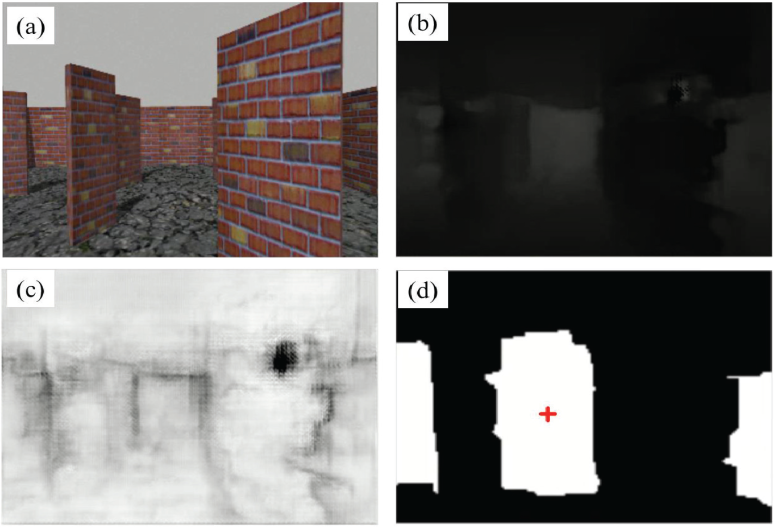
\includegraphics[scale=0.4]{partes/img/P-CNN.png}
    \caption[Mecanismo de evasión de obstáculos por CNN probabilística.]{Mecanismo\footnotemark de evasión de obstáculos por CNN probabilística \cite{Yang2021}. \textbf{(a)} Imagen RGB. \textbf{(b)} Mapa de profundidad. \textbf{(c)} Mapa de confianza. \textbf{(d)} Mascara de obstáculos y dirección de navegación seleccionada (cruz roja).} 
    \label{fig:P-CNN}
\end{figure}
\footnotetext{Obtenida de: \cite{Yang2021}}

El mecanismo de evasión de obstáculos por CNN probabilística propuesto en \cite{Yang2021} demostró ser efectivo para navegación arbitraria en interiores, sin embargo, como este método no considera el objetivo de la navegación, resulta poco útil para la mayoría de las aplicaciones.

Métodos que utilizan aprendizaje por reforzamiento abordan el problema de la evasión de obstáculos utilizando solamente la información disponible a bordo del QUAV. En \cite{Tu2023} se utiliza un algoritmo basado en \textit{Q-learning} para entrenar un agente dedicado a la evasión de obstáculos de un QUAV, donde la observación del estado del entorno viene dada por un mapa de profundidad y una imagen RGB; y donde el espacio de acciones es discreto, cada una representando una dirección de movimiento con respecto al campo de visión del QUAV. De forma similar, en \cite{Xue2021} se utiliza un algoritmo basado en el método Actor-Crítico suave (del inglés \textit{Soft Actor-Critic}), utilizando mapas de profundidad como observaciones del entorno pero utilizando un espacio de acciones continuas, donde una acción codifica un rango continuo de movimientos en las direcciones de los ejes \jim{y} y \jim{z} con respecto al marco de referencia del QUAV. 

El proceso de entrenamiento de estos métodos es considerablemente complicado, requiriendo múltiples redes neuronales para su funcionamiento. En la figura \ref{fig:prev-rl-training-process} se muestra el diagrama de flujo del proceso de entrenamiento utilizado en \cite{Xue2021}. Podemos observar inmediatamente la complejidad del proceso, requiriendo el entrenamiento simultaneo de siete CNNs. Otro inconveniente de estos métodos es la sensibilidad a la definición de la función de recompensa y las restricciones producidas por la representación del espacio de acciones.

\begin{figure}[H]
    \centering
    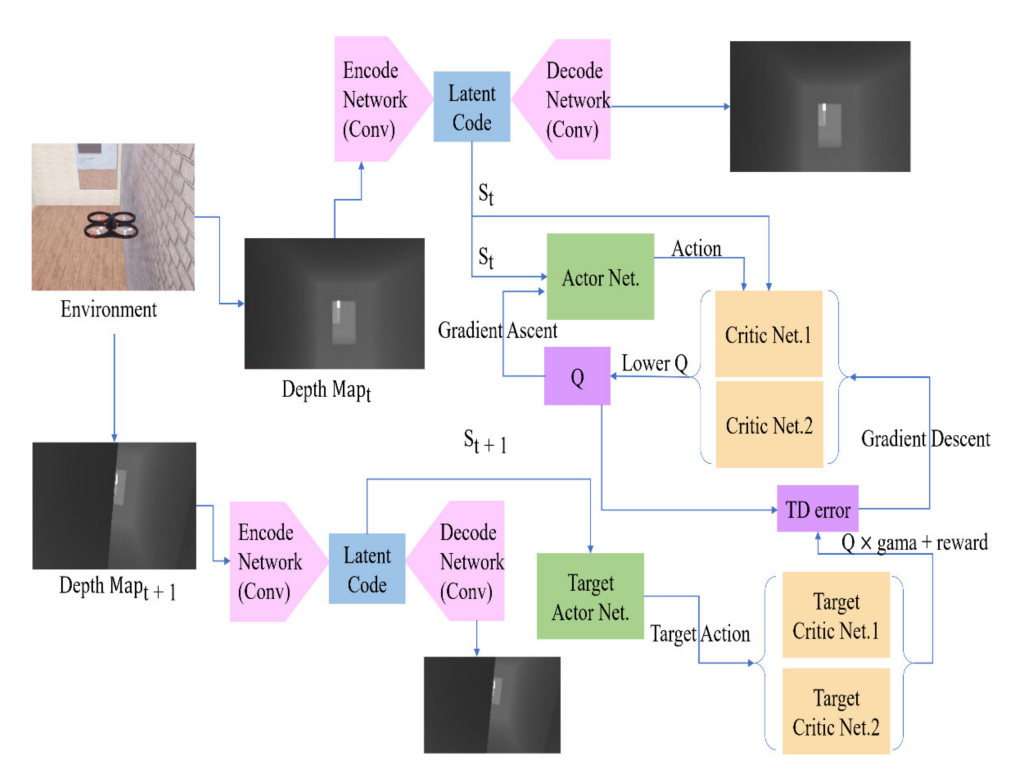
\includegraphics[scale=0.4]{partes/img/RL-training-process.png}
    \caption[Diagrama de flujo del proceso de entrenamiento utilizado en \textit{Vision Based Drone Obstacle Avoidance by Deep Reinforcement Learning}]{Diagrama de flujo del proceso de entrenamiento utilizado en \cite{Xue2021}.}
    \label{fig:prev-rl-training-process}
\end{figure}

Otro método que depende solamente de la información disponible a bordo del vehículo es \textit{Learning high-speed flight in the wild}, propuesto en \cite{Loquercio2021}, este método utiliza una variante del entrenamiento supervisado denominado entrenamiento por imitación (\textit{Imitation Learning} en inglés), en donde se genera una base de datos de entrenamiento utilizando un ``experto'' privilegiado dentro de un ambiente de simulación, para posteriormente aplicar entrenamiento supervisado sobre una política ``estudiante'' cuyo objetivo es aprender a generar trayectorias libres de colisión a partir de un mapa de profundidad del entorno y la mediciones inerciales del QUAV. En la siguiente sección, se profundiza en este método, que resulta ser el principal antecedente del desarrollo del presente trabajo.

\section{\textit{Learning high-speed flight in the wild}}

\label{sec::prev-agile-autonomy}

Tal como se menciono anteriormente, \textit{Learning high-speed flight in the wild} \cite{Loquercio2021} es un método que utiliza entrenamiento por imitación para entrenar una política de generación de trayectorias libres de colisión, a partir de base de datos de ejemplos, que son generados por un experto privilegiado dentro de un entorno de simulación. La figura \ref{fig:prev-agile-autonomy-overview} ilustra el funcionamiento de este método donde se aprecian sus tres componentes principales: El experto privilegiado, la política estudiante y la proyección de trayectorias. En las siguientes secciones se profundiza en el funcionamiento de cada uno de estos componentes.

\begin{figure}[H]
    \centering
    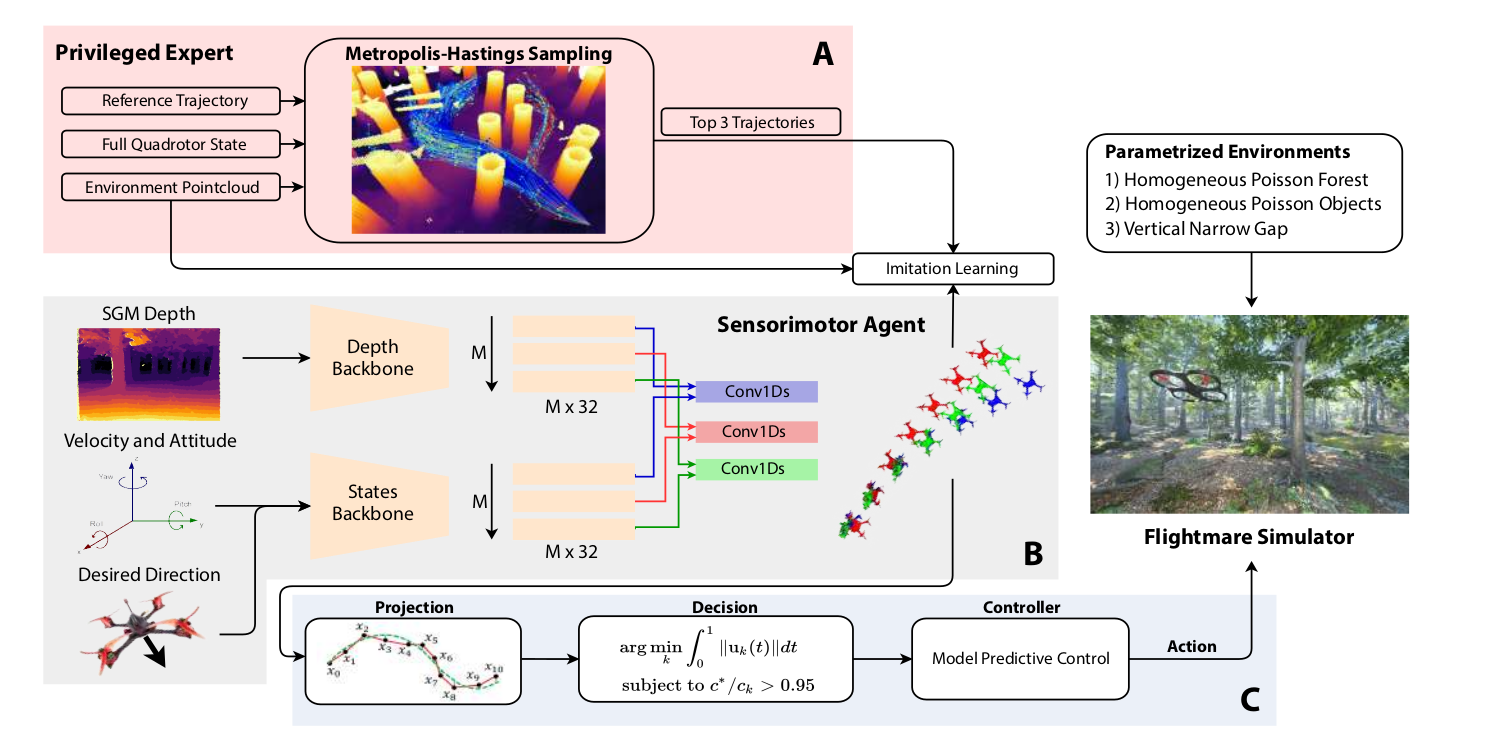
\includegraphics[scale=0.3]{partes/img/agile-autonomy-overview.png}
    \caption[Visión general del método propuesto en \textit{Learning high-speed flight in the wild}]{Visión general del método propuesto en \textit{Learning high-speed flight in the wild} \cite{Loquercio2021}. \textbf{(A)} El experto privilegiado genera una distribución de trayectorias libre de colisión que siguen una trayectoria de referencia. Las trayectorias generadas están condicionadas por la completa información de obstáculos del entorno. \textbf{(B)} La política estudiante es entrenada mediante entrenamiento supervisado para predecir las mejores tres trayectorias a partir un mapa de profundidad, mediciones inerciales del dron y una dirección objetivo. \textbf{(C)} Durante la ejecución, las predicciones de la política estudiante son proyectadas en el espacio de las trayectorias polinomiales y finalmente la trayectoria con el costo de predicción mas bajo es ejecutada por el modelo de control. }
    \label{fig:prev-agile-autonomy-overview}
\end{figure}

\subsection{El experto privilegiado} 

El experto privilegiado es un algoritmo de planificación de trayectorias basado en muestreo \cite{Loquercio2021}. El experto tiene conocimiento completo del estado del QUAV y de la configuración tridimensional del entorno (en forma de una nube de puntos tridimensional). El experto genera trayectorias libres de colisión \jim{\tau} que representan el estado deseado del QUAV \jim{x_{des} \in \mathbb{R}^{13}} durante el siguiente segundo, comenzando desde el estado inicial de QUAV, en otras palabras \jim{\tau(0) = x_0}. Para realizar esta tarea, se toman muestras de una distribución \jim{P} que codifica la distancia a los obstáculos y la proximidad a la trayectoria de referencia; esto es, la distribución \jim{P(\tau | \tau_{ref}, \mathcal{C})} es condicionada por la trayectoria de referencia \jim{\tau_{ref}} y la nube de puntos del entorno \jim{\mathcal{C} \in \mathbb{R}^{n \times 3}}. De acuerdo \jim{P}, la probabilidad de una trayectoria \jim{\tau} es alta si esta lejos de obstáculos en \jim{\mathcal{C}} y cerca de \jim{\tau_{ref}}. La ecuación \ref{eq:aoa-expert-P} muestra la definición de \jim{P} \cite{Loquercio2021}.

\begin{equation}
\label{eq:aoa-expert-P}
    P(\tau | \tau_{ref}, \mathcal{C}) = \frac{1}{Z} e^{-c(\tau, \tau_{ref}, \mathcal{C})}
\end{equation}

Donde \jim{Z = \int_{\tau} P(\tau | \tau_{ref}, \mathcal{C})} es el factor de normalización y \jim{c(\tau, \tau_{ref}, \mathcal{C}) \in \mathbb{R}^{+}} es una función de costo que indica la proximidad a la trayectoria de referencia y la distancia a los obstáculos. En la ecuación \ref{eq:aoa-expert-cost} define \jim{c} de acuerdo a \cite{Loquercio2021}.

\begin{equation}
\label{eq:aoa-expert-cost}
\begin{split}
    c(\tau, \tau_{ref}, \mathcal{C}) &  = \int_{0}^{1}{\lambda_{c} C_{collision}(\tau(t), \mathcal{C}) \, dt} \\
                                     & + \int_{0}^{1}{[\tau(t), - \tau_{ref}(t)]^{T} \, \mathcal{Q} \, [\tau(t) - \tau_{ref}(t)] \, dt}
\end{split}
\end{equation}

Donde \jim{\lambda_c = 1000}, \jim{\mathcal{Q}} es una matriz positiva que representa los pesos de los componentes del estado del vehículo, y \jim{C_{collision}} una función que cuantifica la distancia del QUAV a los puntos de \jim{\mathcal{C}}. Si \jim{r_q} es el radio del QUAV y \jim{d(z, \mathcal{C})} es la distancia de \jim{z \in \mathbb{R}^{3}} al punto mas cercano en \jim{\mathcal{C}}, la ecuación \ref{eq:aoa-expert-distance} define \jim{C_{collision}} de acuerdo a \cite{Loquercio2021}.

\begin{equation}
\label{eq:aoa-expert-distance}
    C_{collision}(\tau(t), \mathcal{C}) = \begin{cases}
        0                                               & \quad\text{\textbf{si} } d(\tau(t), \mathcal{C}) > 2 r_q \\
        4 - (\frac{d(\tau(t), \mathcal{C})}{r_q})^{2}   & \quad\text{\textbf{si} } d(\tau(t), \mathcal{C}) \leq 2 r_q
    \end{cases}
\end{equation}

Debido a que generalmente existe mas de una forma para evadir un obstáculo, la distribución es \jim{P} es multi-modal, haciendo que el calculo analítico de \jim{P} sea difícil de resolver. Para aproximar la densidad \jim{P}, el experto utiliza muestreo aleatorio mediante el algoritmo de \textit{Metropolis-hastings} \cite{hastings1970monte}. Para estimar \jim{P}, el algoritmo de \textit{Metropolis-hastings} necesita una función objetivo \jim{s(\tau) \propto  P(\tau | \tau_{ref}, \mathcal{C})}, en \cite{Loquercio2021} se utiliza \jim{s(\tau) = e^{-c(\tau, \tau_{ref}, \mathcal{C})}}. Luego, \cite{Loquercio2021} muestra que este algoritmo estima asintóticamente la distribución \jim{P}, por lo tanto, se asegura que las muestras de trayectorias cubren asintóticamente todas las modas de \jim{P}.

Para reducir la dimensionalidad del problema, el experto representa las trayectorias \jim{\tau} como curvas de Bezier con tres puntos de control (\jim{\tau \in \mathbb{R}^{3 \times 3}}) tal como se establece en \cite{mellinger2011minimum}, la longitud de estas trayectorias esta determinada por la rapidez promedio de ejecución deseada del QUAV. Adicionalmente, para reducir la complejidad de ejecución del experto, se discretizan las trayectorias en segmentos equitativamente espaciados de 0.1 segundos de duración y se evalúa la versión discreta de la ecuación \ref{eq:aoa-expert-cost}.

El experto luego se utiliza para generar una base de trayectorias libres de colisión mediante su ejecución en línea dentro de un ambiente de simulación. La figura \ref{fig:prev-aoa-expert-sample} se visualiza las muestras de \jim{P} generadas por el experto durante un paso de la simulación. Como trayectoria de referencia se utiliza una trayectoria global libre de obstáculos que se calcula utilizando el método de \cite{liu2018search} que comienza en una posición inicial y termina en la posición objetivo dentro del entorno. Se repite este proceso múltiples veces sobre distintos entornos de simulación. 

\begin{figure}[H]
    \centering
    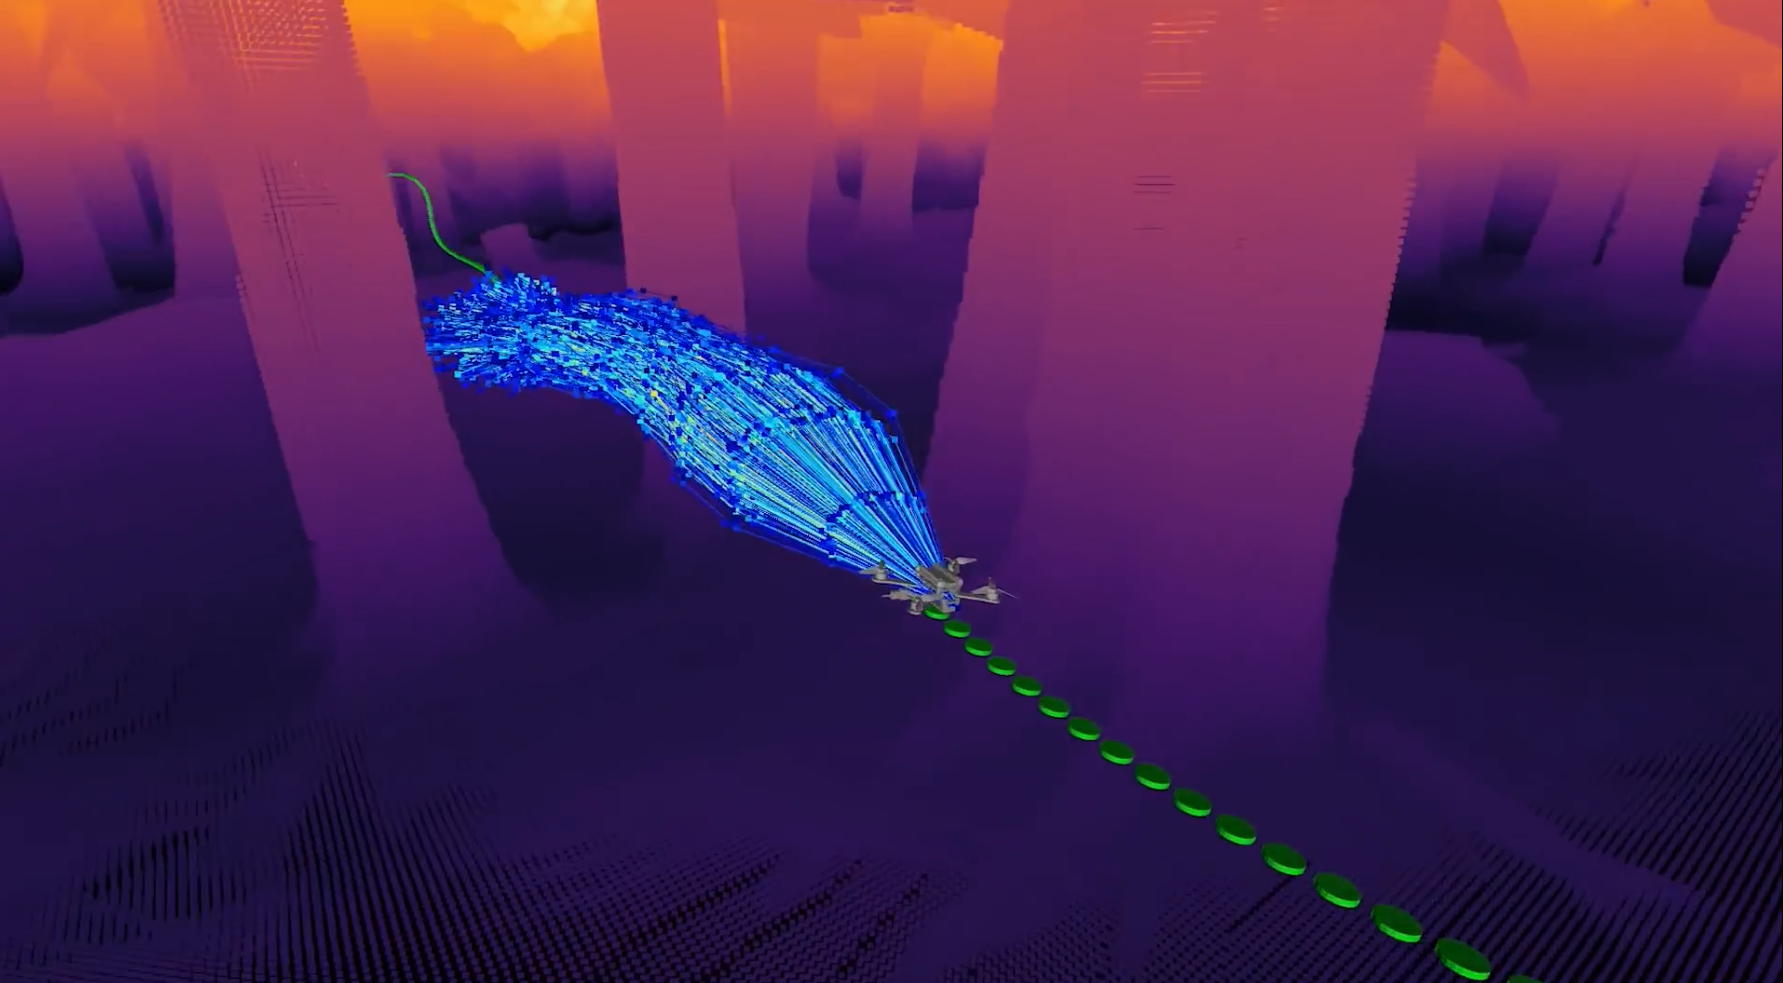
\includegraphics[scale=0.2]{partes/img/aoa-expert-sample.png}
    \caption[Visualización de las muestras de \jim{P} generadas por el experto durante un paso de la simulación.]{Visualización de las muestras de \jim{P} generadas por el experto durante un paso de la simulación. Los puntos verdes representan \jim{\tau_{ref}}.}
    \label{fig:prev-aoa-expert-sample}
\end{figure}


El conjunto de las mejores trayectorias generadas (mejores tres muestras por cada paso de la simulación) a lo largo de todas las ejecuciones se utiliza para formar una base de datos de trayectorias libres de colisión, cada ejemplo de la base de datos viene acompañado de un mapa de profundidad que se genera utilizando visión estereoscópica y del estado del QUAV (velocidad, rotación, posición y dirección objetivo). Si los entornos de simulación donde se realizan ejecuciones son los suficientemente variados (bosques, entornos urbanos, entornos de desastre, objetos aleatorios, entre otros) la base datos generada tiene la capacidad de utilizarse para entrenar políticas de evasión de obstáculos con un nivel de generalización aceptable \cite{Loquercio2021}. Es importante mencionar que debido a que la longitud de las muestras de \jim{P} están condicionadas por la rapidez promedio de ejecución deseada del QUAV, distintas velocidades de ejecución requieren diferentes base de datos, en otras palabras, para cada rapidez promedio de ejecución se necesita generar una base de datos distinta, y por lo tanto, las políticas de evasión de obstáculos entrenadas usando este método están condicionadas a la rapidez promedio del QUAV utilizada durante la generación de la base de datos.

\subsection{La política estudiante} 

\label{sec:aoa-student}

En contraste con el experto, la política estudiante (el estudiante) produce trayectorias libres de colisión en tiempo real utilizando solamente la información de los sensores disponible a bordo del QUAV. La información sensorial utilizada por el estudiante incluyen: un mapa de profundidad estimado utilizando visión estereoscópica, la velocidad y rotación del QUAV, y una dirección objetivo que es representada como un vector unitario que apunta hacia un punto de referencia un (1) segundo en el futuro con respecto al ultimo estado conocido del QUAV. Utilizando esta información y alguna base de datos generada por el experto privilegiado se puede entrenar un modelo que pueda cumplir con los requerimientos de la política estudiante.

En \cite{Loquercio2021} se modela la política estudiante como una red neuronal. La arquitectura de esta red contiene dos ramas que codifican distintas características: una rama convolucional, que codifica la información visual del entorno a partir de un mapa de profundidad \jim{D \in \mathbb{R}^{640 \times 480}}; y una rama que codifica el estado del QUAV a partir de la velocidad del vehículo \jim{v \in \mathbb{R}^{3}}, la rotación expresada como una matriz \jim{q \in \mathbb{R}^{9}}, y la dirección objetivo \jim{r \in \mathbb{R}^{3}} tal que \jim{\|r\| = 1}. 

La rama convolucional utiliza una instancia pre-entrenada de MobileNetV3 \cite{Howard2019} para extraer eficientemente las características visuales del mapa de profundidad. Estas características son posteriormente procesadas por una capa convolucional 1D para generar 3 vectores de tamaño 32, cada uno representando una moda de \jim{P}. 

La rama del estado del QUAV concatena \jim{v}, \jim{q} y \jim{r} y procesa el resultado mediante una red FC de 4 capas, cada una con \jim{[64,32,32,32]} numero de nodos y activaciones LeakyReLU; posteriormente el resultado es procesado por una capa convolucional 1D para generar 3 vectores de tamaño 32, una vez mas, cada uno representando una moda de \jim{P}.

Para cada moda, las codificaciones de la rama de estado y de la rama convolucional se concatenan y son procesadas por una red FC de 3 capas, cada una con \jim{[64,128,128]} numero de nodos y activaciones LeakyReLU. Finalmente, una ultima capa FC con activación LeakyReLU predice una trayectoria \jim{\tau} y costo de ejecución análogo al costo definido en la ecuación \ref{eq:aoa-expert-cost}. 


La salida de la red representa \jim{\mathbb{T}_n = \{ (\tau_{n}^{k}, c_k) | \, k \in [0,1,2] \}}, donde \jim{c_k \in \mathbb{R}^{+}} es el costo de ejecución de la trayectoria \jim{\tau_{n}^{k}} (análogo al definido en la ecuación \ref{eq:aoa-expert-cost}), nótese que cada \jim{k} representa una moda de \jim{P}. A diferencia del experto, las trayectorias predichas por el estudiante describen solamente el componente de la posición de la trayectoria, por esto, \jim{\tau_{n}^{k} \in \mathbb{R}^{10 \times 3}} y describe:

\begin{equation}
\label{eq:aoa-network-taun}
    \tau_{n}^{k} = {[p(t_i)]}_{i = 1}^{10}, \, t_i = \frac{i}{10}
\end{equation}

Donde \jim{p(t_i) \in \mathbb{R}^{3}} es la posición del QUAV en el tiempo \jim{t = t_i} relativo al estado actual \jim{x_0}.

La red neuronal se entrena utilizando entrenamiento supervisado por descenso de gradiente. La función de pérdida para el entrenamiento tiene dos componentes, uno que representa el costo espacial entre la trayectoria predicha y la trayectoria generada por el experto; y otro que representa el costo de estimación de la función \jim{c} (definida en la ecuación \ref{eq:aoa-expert-cost}).

El componente espacial de la función de pérdida es de tipo ``el ganador gana todo'' relajada R-WTA (del inglés \textit{Relaxed Winner-Takes-All)} definida como:

\begin{equation}
\label{eq:aoa-student-spacial-loss}
    \text{R-WTA}(\mathbb{T}_e, \mathbb{T}_n) = \sum_{i=0}^{|\mathbb{T}_e|} \sum_{k=0}^{|\mathbb{T}_n|} \alpha(\tau_{e,p}^{i}, \tau_{n}^{k}) {\|\tau_{e,p}^{i} - \tau_{n}^{k}\|}^2
\end{equation}

Donde \jim{\mathbb{T}_e} y \jim{\mathbb{T}_n} son el conjunto de trayectorias producidas por el experto y por el estudiante respectivamente, \jim{\tau_{e,p}} es el componente de la posición de \jim{\tau_e} y \jim{\alpha(.)} se define como:

\begin{equation}
\label{eq:aoa-student-spacial-alpha}
    \alpha(\tau_{e,p}^{i}, \tau_{n}^{k}) = \begin{cases}
        1 - \epsilon                            & \quad\text{\textbf{si} } {\|\tau_{e,p}^{i} - \tau_{n}^{k}\|}^2 \leq {\|\tau_{e,p}^{j} - \tau_{n}^{k}\|}^2 \, \forall i \ne j \\
        \frac{\epsilon}{|\mathbb{T}_n| - 1}     & \quad\text{\textbf{en caso contrario}}
    \end{cases}
\end{equation}

Con \jim{\epsilon = 0.05}. Esta definición hace que intuitivamente se asocie una trayectoria \jim{\tau_{e}^{i} \in \mathbb{T}_e} con la trayectoria mas cercana predicha por el estudiante \jim{\tau_{n}^{k} \in \mathbb{T}_n}, asignándole un peso de \jim{1 - \epsilon = 0.95}; dejando un peso de \jim{\epsilon / (|\mathbb{T}_n| - 1) = 0.025} para el resto de las predicciones, de ahí el nombre ``el ganador gana todo''. Esta formulación permite que la red pueda aprender el comportamiento multi-modal de las trayectorias generadas por el experto.

El componente de estimación de la función \jim{c} esta dado por la suma de diferencias cuadradas entre el valor a estimar y la predicción de la red. El valor a estimar se obtiene para cada predicción utilizando la asociación generada por el componente R-WTA, digamos que \jim{h(k)} retorna el índice de la trayectoria del experto asociada con la predicción numero \jim{k}. Finalmente, la función de pérdida utilizada para el entrenamiento de la red neuronal que modela al estudiante es \cite{Loquercio2021}:

\begin{equation}
\label{eq:aoa-student-spacial-loss-full}
    L(\mathbb{T}_e, \mathbb{T}_n) = 10 \cdot \text{R-WTA}(\mathbb{T}_e, \mathbb{T}_n) + \frac{1}{10} \cdot \sum_{k=0}^{|\mathbb{T}_e|} [c_k - c(\tau_{n}^{k}, \tau_{e,p}^{h(k)}, \mathcal{C})]^2
\end{equation}

Esta función de pérdida es promediada sobre un \textit{batch} de 8 muestras y se minimiza utilizando descenso de gradiente con una tasa de aprendizaje de \jim{1 \times 10^{-3}} \cite{Loquercio2021}.

\subsection{Proyección de trayectorias} 

\label{sec:prev-aoa-traj}

Las trayectorias predichas por la política estudiante son proyectadas al espacio de los polinomios de grado \jim{N} con \jim{N \geq 3} para cada eje independientemente. Esta representación polinómica asegura continuidad en posición, velocidad, aceleración y facilita la viabilidad dinámica de la trayectoria \cite{mellinger2011minimum}. Por ejemplo, para el eje x, se define la proyección polinómica \jim{\mu_x(t) = a_x^T \cdot T(t)}, donde \jim{a_x^T = [a_0, a_1, ..., a_N]} y \jim{T(t) = [1, t, ..., t^{N -1}, t^{N}]}. El termino de proyección \jim{a_x} se obtiene resolviendo el siguiente problema de optimización:

\begin{equation}
\label{eq:aoa-traj-proj}
\begin{split}
    \min_{a_x} \sum_{i=1}^{10} & (\tau_{n,x}^{k,i} - a_x^T \cdot T(\frac{i}{10}))^{2} \\
    \text{\textbf{sujeto a:}} & \\
                     & p_x(0) - a_x^T \cdot T(0) = 0 \\
                     & v_x(0) - a_x^T \cdot \frac{dT}{dt}(0) = 0 \\
                     & a_x(0) - a_x^T \cdot \frac{d^2 T}{{dt}^2}(0) = 0 \\
\end{split}
\end{equation}

Donde \jim{\tau_{n,x}^{k,i}} es el componente en el eje x del elemento numero \jim{i} de \jim{\tau_{n}^{k}}, y \jim{p_x(0), v_x(0), a_x(0)} son el componente x de la posición, velocidad y aceleración del QUAV obtenidas del ultimo estado \jim{x_0}. Adicionalmente, para evitar cambios abruptos en la velocidad durante el vuelo, se limita la rapidez promedio del polinomio a un valor definido \jim{v_{des}} que coincide con la rapidez promedio de ejecución de la base de datos con la que se entrenó la política estudiante. Para ello, se escala el tiempo \jim{t} del polinomio \jim{\mu(t)} por un factor \jim{\beta = v_{des} / v_\mu} donde \jim{v_\mu = \| \mu(0) - \mu(1) \|}.

Una vez que todas las trayectorias han sido proyectadas, se escoge una para ejecutarse. Para esto, se seleccionan las trayectorias que cumplan con \jim{c^{*} / c_k \geq 0.95 \, (c^{*} = \min_k c_k)} y se selecciona aquella de que tenga el menor valor de entrada acuerdo al criterio establecido por \cite{mellinger2011minimum}. Esto refuerza continuidad temporal de las trayectorias. Por ejemplo, si se esta esquivando un obstáculo por la derecha no es ideal navegar hacia la izquierda en la siguiente iteración, a no ser que sea estrictamente necesario por la apariencia del obstáculo. Finalmente, se obtienen valores de posición, velocidad y aceleración de la trayectoria seleccionada y se envían al FCU para su ejecución.

\section{Resumen}

Este capítulo abordó el problema de la evasión de obstáculos, centrándose en dos variantes de planificación local de caminos: aquellas que requerían información global previa y las que se basaban únicamente en la información de los sensores a bordo del vehículo. La sección \ref{sec::prev-global} exploró desarrollos relacionados con la primera variante, mientras que la sección \ref{sec::prev-local} se centró en la segunda. Además, se profundizó en \textit{Learning high-speed flight in the wild} en la sección \ref{sec::prev-agile-autonomy}, destacando su papel como un antecedente crucial para el desarrollo del presente trabajo. Este capítulo proporcionó una visión del estado actual en el campo, resaltando las perspectivas relevantes para la resolución del problema de evasión de obstáculos para QUAVs.

En el siguiente capítulo se describirá la implementación de la solución propuesta por este trabajo, teniendo en cuenta el contexto de la plataforma disponible, así como también fundamentando la selección del algoritmo de evasión de obstáculos y detallando sus componentes de implementación.
    
   
\chapter{Implementación}
\label{capitulo5}
\lhead{Capítulo 5. \emph{Implementación}}

En el capítulo anterior se realiza una revisión del estado del arte de los algoritmos de evasión de obstáculos en el contexto de los QUAVs. En este capítulo se hace la descripción de la implementación de la solución propuesta, para el problema de evasión de obstáculos sobre el contexto de la plataforma de implementación de los productos de ACSL. En la Sección \ref{sec:imp-platform} se describe brevemente la metodología y plataforma de implementación; en la Sección \ref{sec:imp-algo} se fundamenta la selección del algoritmo de evasión de obstáculos, inspirado en \textit{Learning high-speed flight in the wild} \cite{Loquercio2021}; en la Sección \ref{sec:imp-arch} se describe la arquitectura de la solución propuesta en este trabajo, así como también se describe el funcionamiento de cada uno de sus componentes; y finalmente en la Sección \ref{sec:imp-finetune} se describe el proceso de refinamiento fino de la red neuronal encargada de la inferencia de trayectorias libre de colisión, es decir, el ajuste fino de la política estudiante.

\section{Plataforma de implementación}

\label{sec:imp-platform}

El componente principal de la metodología de implementación de soluciones sobre los productos de ACSL, es una librería propietaria de ACSL llamada \textit{ACSL Vision Core}. Esta librería, escrita en C++, proporciona un marco de trabajo para la implementación de aplicaciones sobre los UAV de ACSL, adicionalmente admitiendo el uso de vehículos simulados por el entorno de simulación AirSim \cite{shah2018airsim}. Bajo este marco de trabajo, una solución es implementada como una colección de procesos de linux independientes que se comunican utilizando memoria compartida y \textit{sockets} de la librería ZeroMQ \cite{zeroMQ}. La implementación del algoritmo a seleccionar debe estar condicionada a este marco de trabajo, para que la solución propuesta pueda ejecutarse en concordancia y con capacidad de interacción con otras aplicaciones de los vehículos de ACSL. La libreria \textit{ACSL Vision Core} expone un API (Interfaz de programación de aplicación, del inglés \textit{Aplication Programming Interface}) llamada \textit{ACSL Flight API} que permite interactuar con el FCU\footnote{Unidad de control de vuelo, tal como se define en la Sección \ref{sec:QUAV-FCU}} del QUAV, exponiendo métodos para leer la información de la estimación del estado del QUAV (posición, velocidad, rotación y estado de los actuadores) y para enviar comandos de control de alto nivel desde un proceso ejecutándose en el computador a bordo del vehículo.

\subsection{Plataforma física}

El vehículo sobre el cual se implementó la solución propuesta en el presente trabajo es SOTEN, un QUAV de tamaño ligero diseñado por ACSL para aplicaciones de fotografía aérea (Inspección, vigilancia, rescate, entre otros). En la Figura \ref{fig:SOTEN} se muestra una imagen del vehículo en cuestión.

\begin{figure}[H]
    \centering
    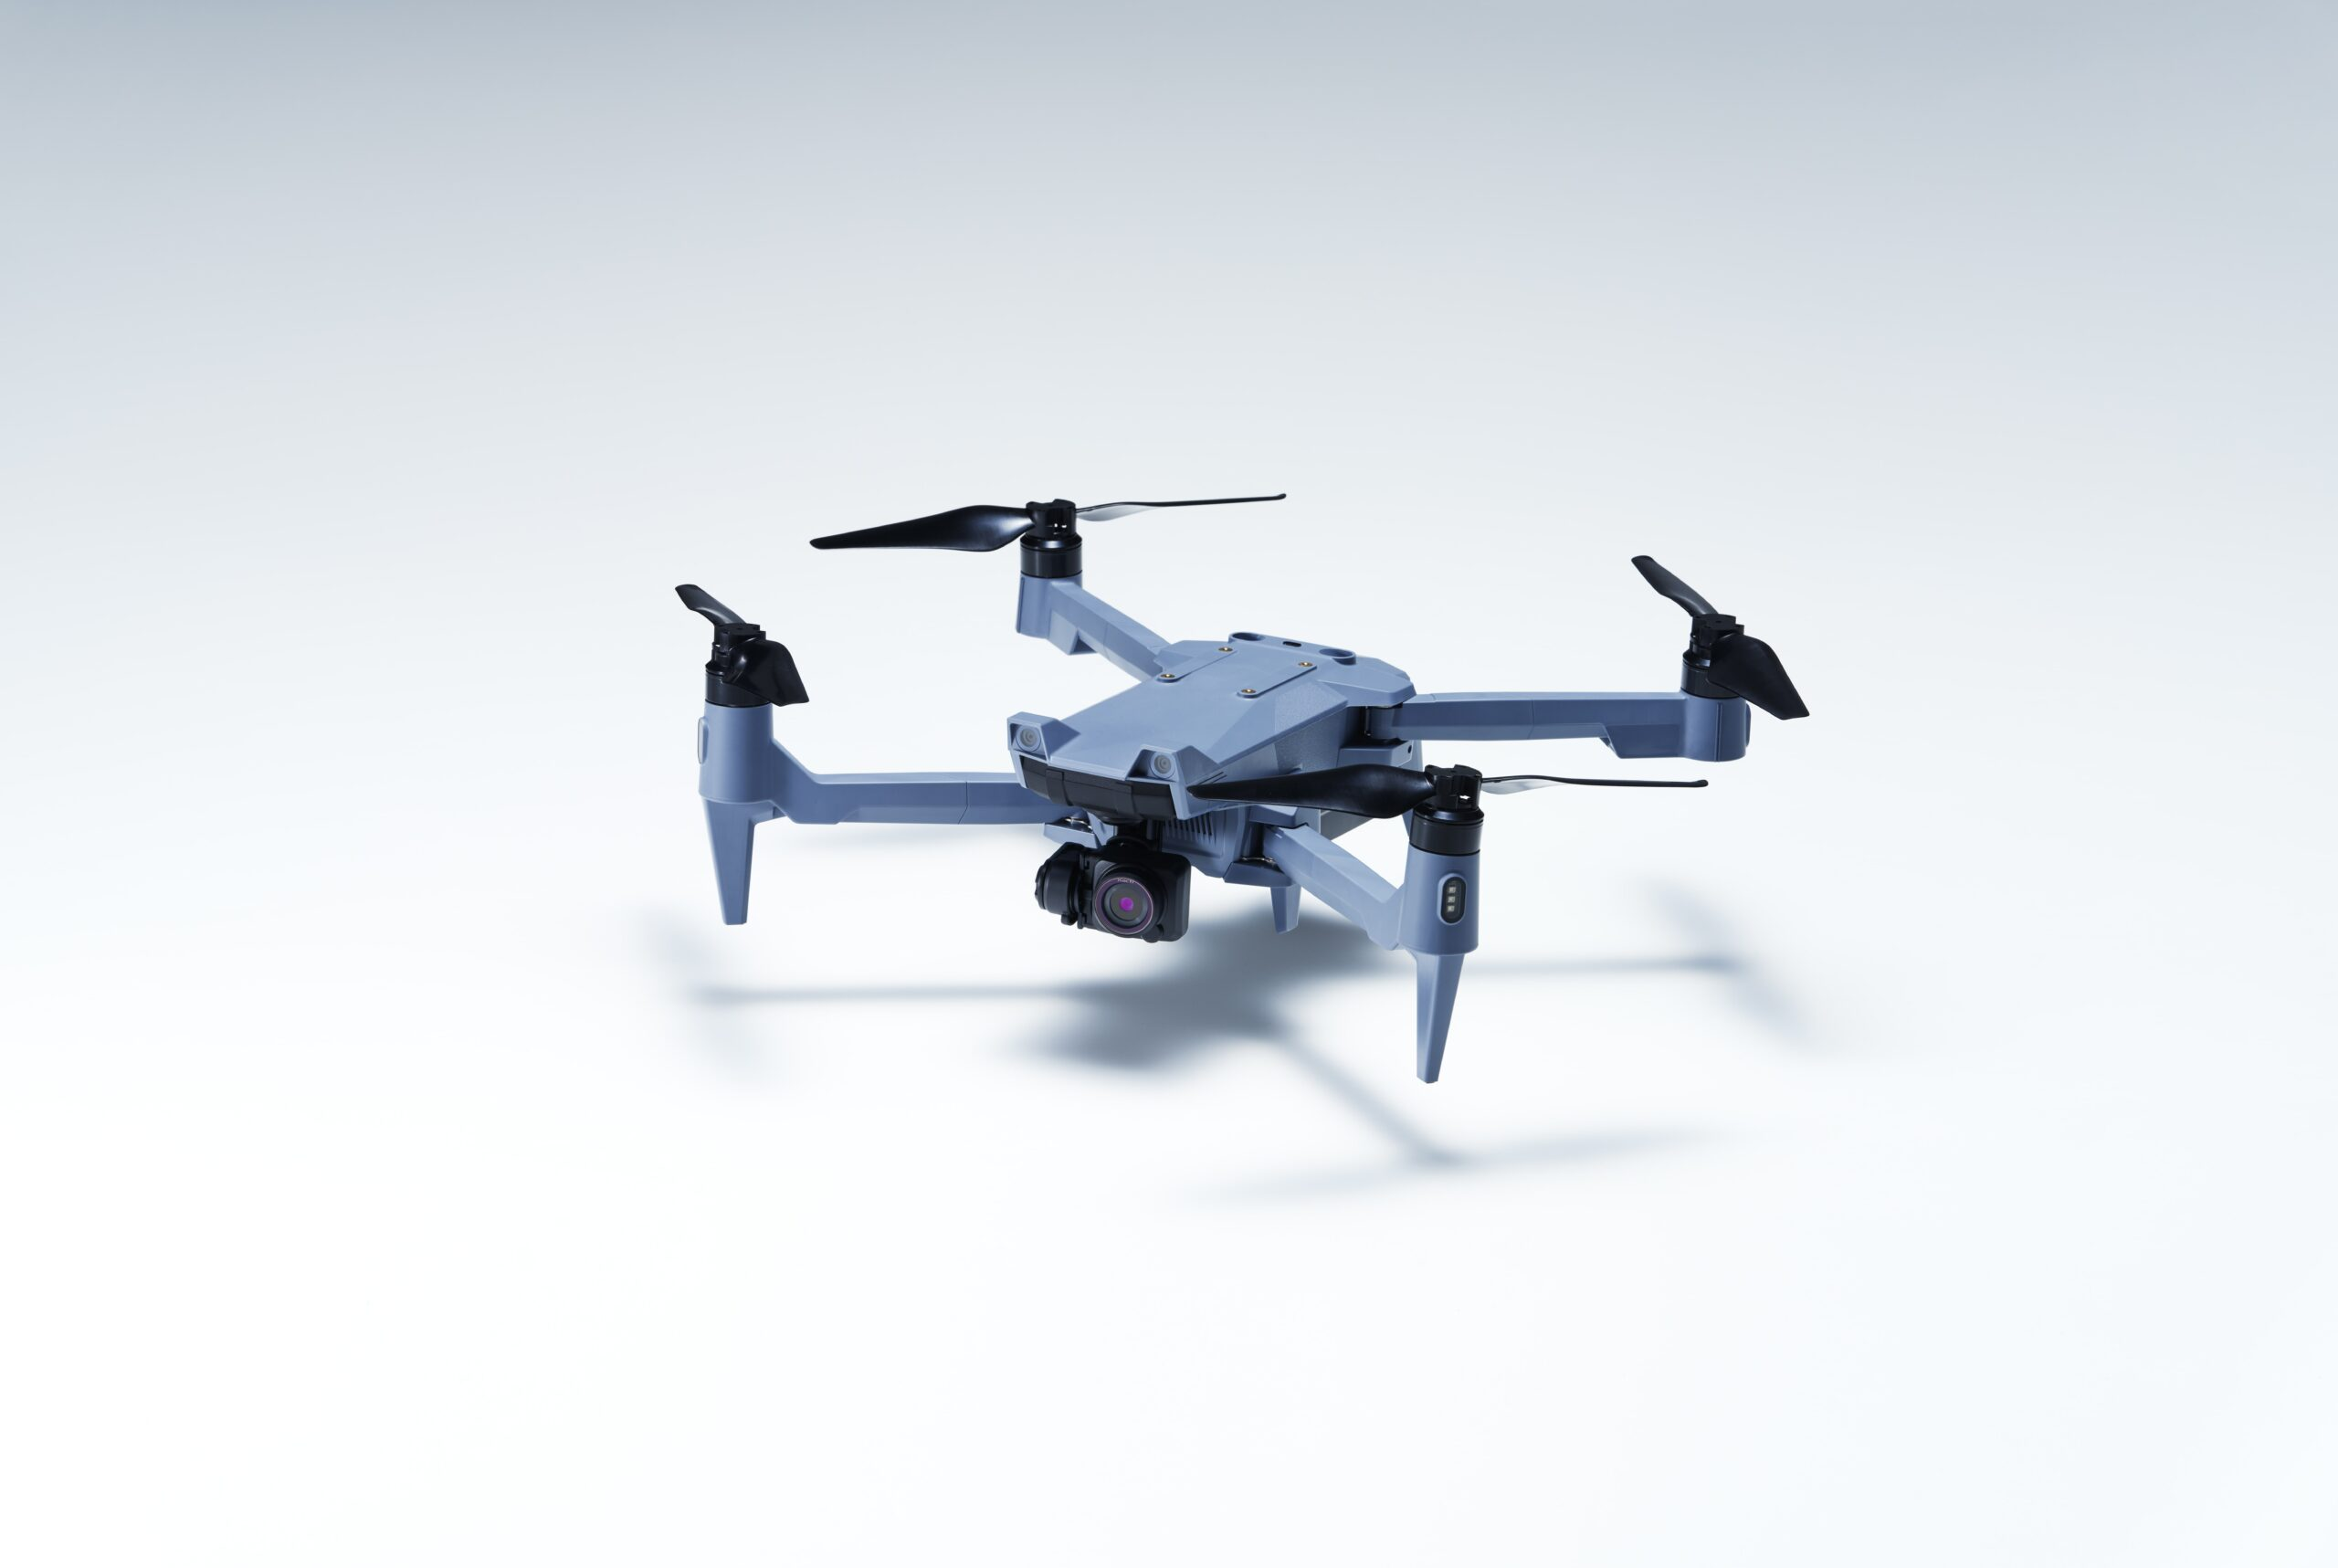
\includegraphics[scale=0.13]{partes/img/SOTEN.jpg}
    \caption[SOTEN, un QUAV diseñado por ACSL que sirve de plataforma física para la implementación de este trabajo.]{SOTEN, un QUAV diseñado por ACSL que sirve de plataforma física para la implementación de este trabajo.}
    \label{fig:SOTEN}
\end{figure}

SOTEN viene equipado con un chip NVIDIA Jetson Xavier NX, que funciona como computadora a bordo del QUAV, que posee capacidades de aceleración gráfica y es precisamente donde se implementó la solución propuesta en este trabajo. Con respecto a los sensores, SOTEN viene equipado con un conjunto de cámaras estereoscópicas, de las cuales en este trabajo solo se utilizó el par frontal; así como también se equipa de una cámara de inspección estabilizada por un \textit{gimbal} que si bien no es utilizada en este trabajo, representa una de las funciones principales de SOTEN, su capacidad de inspección. Como mecanismo de localización tiene acceso a locación por GPS y localización por visión, en este trabajo solo se utilizó la localización por GPS. 

\subsection{Entorno de simulación}

El entorno de simulación que es soportado por \textit{ACSL Vision Core} es AirSim \cite{shah2018airsim}, donde se pueden simular una variedad de vehículos equivalentes a los productos de ACSL en entornos de simulación ejecutados por \textit{UnrealEngine}. En este trabajo se utiliza AirSim para simular un QUAV equivalente a SOTEN, que permite que dentro de las simulaciones se tengan las mismas propiedades dinámicas y dimensiones de la plataforma física. La implementación de la solución propuesta en este trabajo es agnóstica de la utilización de AirSim, el \textit{ACSL Flight API} se encarga de traducir los comandos de control al equivalente en el marco de trabajo del simulador.

\section{Selección del algoritmo}

\label{sec:imp-algo}

El algoritmo seleccionado sigue al propuesto en \textit{Learning high-speed flight in the wild} \cite{Loquercio2021}. Las características del método propuesto en \cite{Loquercio2021} resultan atractivas para los productos de ACSL, en concreto: solo requiere de la información disponible a bordo del vehículo; no requiere sensores que alguno de los productos de ACSL no tenga disponible; tiene la capacidad de adaptarse a aplicaciones específicas si se escogen adecuadamente los entornos de simulación para la generación de la base datos; como la información visual se representa en forma de un mapa de profundidad, es sencillo trasladar el algoritmo entre plataformas; y finalmente, los autores de \textit{Learning high-speed flight in the wild} dan acceso público al código fuente para la generación de las base de datos y del entrenamiento de la política estudiante, así como también los pesos entrenados de la red neuronal utilizada, reduciendo el trabajo necesario para implementar el algoritmo sobre la plataforma de ACSL.

Sin embargo, es necesario realizar ciertas modificaciones al algoritmo. Primero, por motivos de seguridad es necesario que la rapidez de ejecución esté limitada a 1 m/s, esto es, \jim{v_{des} = 1}; los pesos de la política estudiante publicados en \cite{Loquercio2021} fueron entrenados con \jim{v_{des} = 7}, por lo tanto es necesario hacer un proceso de ajuste fino de los pesos. Segundo, debido a limitaciones del \textit{ACSL Flight API}, solo se puede enviar instrucciones para modificar la referencia de la velocidad y de la velocidad rotacional; a diferencia de \cite{Loquercio2021} en donde se envían instrucciones con referencia de posición, rotación, velocidad y aceleración simultáneamente, por lo tanto, la ejecución de las trayectorias para este trabajo solamente envía la información de la velocidad lineal, junto con un estimado de la velocidad rotacional necesaria para que el encabezado del QUAV apunte hacia la dirección tangencial de la trayectoria en ejecución. Tercero, por motivos de validación del concepto por parte de ACSL, la ejecución de la evasión de obstáculos va a estar limitada al plano \jim{x,y} del marco de referencia del cuerpo del QUAV. En resumen, el algoritmo que se implementa en este trabajo es el mecanismo de inferencia de la política estudiante de \cite{Loquercio2021} luego de un proceso de refinamiento fino; junto con otros componentes implementados dentro del marco de trabajo de ACSL que se encargan de la ejecución de las trayectorias y de la adquisición de la información necesaria para la inferencia.

\section{Arquitectura de la solución}

\label{sec:imp-arch}

Tal como se mencionó en la sección anterior, la solución propuesta por este trabajo es la combinación del mecanismo de inferencia de la política estudiante propuesto por Loquercio et al. \cite{Loquercio2021} y una serie de componentes bajo el marco de trabajo de ACSL encargados de la ejecución de las trayectorias y de la adquisición de la información necesaria para la inferencia. La Figura \ref{fig:sol-comm} muestra el diagrama de comunicación de la solución propuesta; se compone de cuatro componentes: Un puente del FCU, que se encarga de obtener continuamente la última información del estado del QUAV; un puente de profundidad, que procesa los pares de imágenes estéreo producidas por las cámaras frontales para calcular mapas de profundidad; un proceso de inferencia que utiliza la información producida por los puentes de FCU y de profundidad para predecir trayectorias libre de colisión utilizando la red neuronal de \cite{Loquercio2021}; y un ejecutor de trayectorias que ejecuta las trayectorias inferidas por el proceso de inferencia. Los componentes se ejecutan como procesos independientes y se comunican utilizando  \textit{sockets} de la librería ZeroMQ \cite{zeroMQ} y memoria compartida.

\begin{figure}[H]
    \centering
    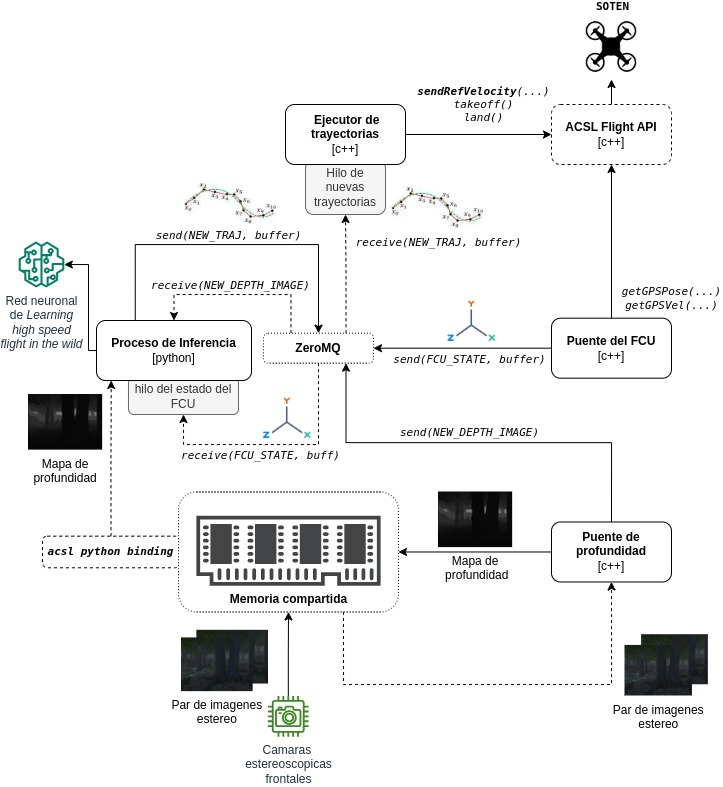
\includegraphics[scale=0.5]{partes/img/Solution-V3-Spanish.jpg}
    \caption[Diagrama de comunicación de la solución.]{Diagrama de comunicación de la solución. En alto nivel, el flujo de información comienza cuando se produce un nuevo par de imágenes estéreo; el puente de profundidad procesa el par para producir un mapa de profundidad; luego el proceso de inferencia recibe el mensaje \texttt{NEW\_DEPTH\_IMAGE}, obtiene la información mas reciente del puente FCU, invoca a la red neuronal y envía el resultado en el mensaje \texttt{NEW\_TRAJ}. Finalmente, el ejecutor de trayectorias, al recibir el mensaje \texttt{NEW\_TRAJ}, proyecta la trayectoria de acuerdo al procedimiento descrito en la Sección \ref{sec:prev-aoa-traj} y procede a ejecutar la trayectoria utilizando el \textit{ACSL Flight API}.}
    \label{fig:sol-comm}
\end{figure}

A continuación se profundiza en cada uno de los componentes.

\subsection{Puente del FCU}

Este componente tiene como función obtener la información mas reciente del estado del QUAV y transmitir dicho estado mediante un \textit{socket} de ZeroMQ para su utilización por el proceso de inferencia. Debido a que el proceso de inferencia se ejecuta en python y el \textit{ACSL Flight API} solo está disponible para entornos de C++, es necesario que un proceso externo obtenga la información del API y se la comunique al proceso de inferencia, esta es justamente la función del puente del FCU.

Si \jim{B} es el marco de referencia del cuerpo del QUAV, a una frecuencia de 120 Hz, este componente invoca las funciones \texttt{getGPSPose} y \texttt{getGPSVel} del \textit{ACSL Flight API} para obtener los estimados mas recientes de: latitud, longitud y altitud (GPS); los ángulos de Euler \textit{roll}, \textit{pitch} y \textit{yaw} de \jim{B}; los componentes \jim{v_{B_x}, v_{B_y}, v_{B_z}} de la velocidad lineal con respecto a \jim{B}; y la velocidad angular del eje \jim{B_z}, \jim{\omega_z}. Adicionalmente, este componente también convierte las coordenadas latitud, longitud, altitud en coordenadas NED utilizando el Algoritmo \ref{alg:NED}, tomando como origen al punto de donde despega el QUAV. Finalmente, estas mediciones son empaquetadas en un \textit{buffer} binario y son enviadas como cuerpo del mensaje \texttt{FCU\_STATE} para su posterior uso por el proceso de inferencia.


\subsection{Puente de profundidad}

Este componente es el encargado de generar los mapas de profundidad necesarios para el funcionamiento del proceso de inferencia. Para realizar esta tarea, obtiene el par más reciente de imágenes estéreo de la cámara frontal, calcula un mapa de disparidad utilizando la funcionalidad de emparejamiento de bloques de la librería \texttt{opencv} \cite{bradski2000opencv}, aplica el método explicado en la Sección \ref{sec:teo-stereo} para obtener un mapa de profundidad a partir del mapa de disparidad y constantes de las cámaras; una vez disponible el mapa de profundidad, se escribe en memoria compartida y envía el mensaje \texttt{NEW\_DEPTH\_IMAGE}, que sirve para notificar al proceso de inferencia que hay un nuevo mapa de profundidad disponible. Este proceso se repite con una frecuencia máxima de 30 Hz, que coincide con la tasa de muestreo del sistema de cámaras estéreo frontales de SOTEN.

\subsection{Proceso de inferencia}

Este componente es el encargado de predecir trayectorias libres de colisión a partir de los mapas de profundidad generados por el puente de profundidad y del estado del QUAV obtenido por el puente del FCU. El procesamiento de este componente se divide en dos hilos: el hilo principal, que realiza inferencia en la red neuronal de \textit{Learning High Speed Flight in the Wild} \cite{Loquercio2021} cada vez que llega el mensaje \texttt{NEW\_DEPTH\_IMAGE}; y el hilo del estado del FCU, que se encarga de recibir los mensajes \texttt{FCU\_STATE} para mantener una copia global del último estado del QUAV.

\subsubsection*{Hilo del estado del FCU}

El procesamiento realizado por este hilo es relativamente simple; cada vez que llega un mensaje \texttt{FCU\_STATE} se obtiene el \textit{buffer} binario del cuerpo del mensaje, se convierte la representación binaria en una representación estructurada y se le asigna a la variable global \texttt{fcu\_state}. La variable \texttt{fcu\_state}, al ser global, es accesible por ambos hilos. Para mantener la integridad de \texttt{fcu\_state} y evitar condiciones de carrera, el acceso de escritura y lectura esta controlado por un semáforo de exclusión mutua (\textit{mutex}).

\subsubsection*{Hilo principal}

El procesamiento del hilo principal puede resumirse en cinco etapas: primero, esperar por un nuevo mensaje de \texttt{NEW\_DEPTH\_IMAGE}; segundo, obtener el último mapa de profundidad de la memoria compartida; tercero, detectar la presencia de obstáculos en el mapa de profundidad, si no existe obstáculo cercano, repetir desde la primera etapa; cuarto, preparar las entradas de la red y realizar inferencia; finalmente, seleccionar las trayectorias que cumplan \jim{c^{*} / c_k \geq 0.95 \, (c^{*} = \min_k c_k)}, codificarlas en un \textit{buffer} binario y enviar un mensaje de \texttt{NEW\_TRAJ} utilizando el \textit{buffer} como cuerpo del mensaje.

La etapa tercera es el resultado de una optimización necesaria para aliviar la carga de procesamiento sobre la computadora a bordo del QUAV. El proceso de realizar inferencia utiliza una porción importante de los recursos de procesamiento del QUAV, si se limita la inferencia exclusivamente a los escenarios donde exista un obstáculo a esquivar, el QUAV puede utilizar los recursos de procesamiento en otras aplicaciones. Para realizar la tarea de detectar obstáculos en un mapa de profundidad, se utiliza un algoritmo que a partir un mapa de profundidad retorna un aproximado de la profundidad al obstáculo mas cercano, este algoritmo asume que los obstáculos mas cercanos aparecen mas grandes en el mapa de profundidad y utiliza la función \texttt{findContours} de la librería \texttt{opencv} \cite{bradski2000opencv} para obtener los contornos de una máscara binaria. Si \jim{\ell} es la distancia máxima en milímetros donde un obstáculo se considera ``cercano'' y \jim{D} es un mapa de profundidad en milímetros, el pseudo-código del algoritmo se muestra en el Algoritmo \ref{alg:nearest-depth}.

\begin{algorithm}
\caption{Pseudo-código del algoritmo para obtener un estimado de la profundidad al obstáculo mas cercano en un mapa de profundidad }
\label{alg:nearest-depth}
\KwData{\jim{D}, \jim{\ell}}
\KwResult{\jim{d}, estimado de la profundidad en metros del obstáculo mas cercano.}

$D_{mask} = D > 10 \wedge D \leq \ell$

\If{$\sum_{(i,j) \in D_{mask}}{D_{mask}(i,j)} > \frac{1}{10} |\{(i,j) \in D\}|$}{
    $\text{\texttt{contornos}} = \text{\texttt{opencv2.findContours(}}D_{mask}\text{\texttt{)}}$ 

    $\text{\texttt{candidato}} = $ el contorno en $\text{\texttt{contornos}}$ con mayor área.

    $a_{cand} = \text{\texttt{candidato.area}}$

    \If{$a_{cand} > \frac{1}{10} |\{(i,j) \in D\}|$}{
        $I_{cont} = \{ (i,j) | (i,j) \in D \wedge (i,j) \in \text{\texttt{candidato}} \}$

        $d = \frac{1}{1000 \cdot |I_{cont}|} \sum_{(i,j) \in I_{cont}}{D(i,j)}$

        \Return{$d$}
    }
}

\Return{\jim{\infty}}

\end{algorithm}

Dicho esto, a continuación se describe el pseudo-código del procedimiento ejecutado por el hilo principal del proceso de inferencia. Dadas las definiciones:

\begin{itemize}
    \item \jim{\Phi: \mathbb{R}^{640 \times 480} \times \mathbb{R}^{15} \longrightarrow \{\mathbb{T}_n |\mathbb{T}_n \text{ es tal como se describe en la Sección \ref{sec:aoa-student}}\}} es una función que representa la red neuronal de \textit{Learning High Speed Flight in the Wild} \cite{Loquercio2021}.
    \item \texttt{fcu\_state} es la variable global que contiene el estado más reciente del QUAV.
    \item \texttt{fcu\_mutex} es el semáforo de exclusión mutua para acceder a \texttt{fcu\_state}.
    \item \jim{\text{\texttt{obs\_distance}}: \mathbb{R}^{640 \times 480} \longrightarrow \mathbb{R^+}} es una implementación del Algoritmo \ref{alg:nearest-depth} con \jim{\ell = 7500} mm.
    \item \jim{\text{\texttt{stop}}: \text{\texttt{void}} \longrightarrow \mathbb{B}} es un predicado que indica si el proceso debe terminar.
    \item \jim{\text{\texttt{aplanar}}: \mathbb{R}^{3 \times 3} \longrightarrow \mathbb{R}^{9}} es una función que transforma una matriz 3x3 en el vector resultante de concatenar sus filas en un vector con nueve coordenadas.
    \item \jim{B} representa el marco de referencia en el cuerpo del QUAV.
\end{itemize}

El pseudo-código del procedimiento ejecutado por el hilo principal del proceso de inferencia se muestra en el Algoritmo \ref{alg:inference-loop}.

\begin{algorithm}
\caption{Pseudo-código del procedimiento ejecutado por el hilo principal del proceso de inferencia. }
\label{alg:inference-loop}
\KwData{\jim{\Phi}, \texttt{fcu\_state}, \texttt{fcu\_mutex}, \texttt{obs\_distance}, \texttt{stop}}

\While{$\neg \text{\texttt{stop}}()$}{
    Esperar a la llegada de un mensaje de \texttt{NEW\_DEPTH\_IMAGE}.

    Obtener \jim{D}, el mapa de profundidad mas reciente en memoria compartida.

    $d = \text{\texttt{obs\_distance}}(D)$

    \If{$d \leq 7.5$}{
        \Continue
    }

    \texttt{fcu\_mutex.incrementar()}

    Utilizar \texttt{fcu\_state} para obtener \jim{V_B \in \mathbb{R}^{3}}, la velocidad del QUAV con respecto a \jim{B}.

    Utilizar \texttt{fcu\_state} para obtener \jim{q \in \mathbb{R}^{9}}, la rotación de \jim{B} en forma de matriz, esto es, \jim{q = \text{\texttt{aplanar(}}R_{\phi}R_{\theta}R_{\psi}\text{\texttt{)}}} donde \jim{\phi,\theta,\psi} son los ángulos de Euler de B.

    Utilizar \texttt{fcu\_state} para obtener \jim{\mu \in \mathbb{R}^{3}}, posición del QUAV en coordenadas NED.

    Utilizar \texttt{fcu\_state} para obtener \jim{\mu_{goal} \in \mathbb{R}^{3}}, la posición del objetivo del vuelo en coordenadas NED.

    Definir la dirección objetivo como \jim{r = \frac{1}{\|\mu_{goal} - \mu\|}(\mu_{goal} - \mu)}.

    \texttt{fcu\_mutex.decrementar()}

    $X = \text{\texttt{concatenar(}}V_B, q, r\text{\texttt{)}}$

    Realizar inferencia sobre la red neuronal $T = \Phi(D, X)$.

    $c^* = \min \, \{c \, | \, (\tau, c) \in T\}$

    $T_f = \{(\tau, c) \, | \, (\tau, c) \in T \wedge c^* / c \geq 0.95 \}$

    Codificar \jim{T_f} en un \textit{buffer} binario \texttt{traj\_buffer}.

    Enviar mensaje \texttt{NEW\_TRAJ} con \texttt{traj\_buffer} como cuerpo del mensaje.
}

\end{algorithm}

Es importante mencionar, que para que la red neuronal de \textit{Learning High Speed Flight in the Wild} \cite{Loquercio2021} pudiera utilizarse sobre la plataforma de SOTEN, fue necesario realizar un proceso de conversión a un formato ligero orientado a la inferencia. Para esto se utilizó el estándar abierto para la interoperabilidad del aprendizaje de máquinas, ONNX \cite{onnx} (del inglés \textit{Open Standard for Machine Learning Interoperability}). De no haberse realizado esta conversión, el proceso de inferencia \textbf{no} podría ejecutarse sobre SOTEN debido a restricciones del \textit{Firmware} del chip NVIDIA Jetson Xavier NX.

\pagebreak

\subsection{Ejecutor de trayectorias}

Este componente es el encargado de ejecutar las trayectorias predichas por el proceso de inferencia, así como también manejar el estado de la ejecución del vuelo. El procesamiento de este componente se divide en dos hilos: el hilo de nuevas trayectorias, que recibe los mensajes de \texttt{NEW\_TRAJ} y proyecta las trayectorias en el espacio de los polinomios de grado \jim{N = 3} de acuerdo a lo especificado en la Sección \ref{sec:prev-aoa-traj}; y el hilo principal, que ejecuta la trayectoria mas reciente y gestiona el estado del vuelo.

\subsubsection*{Hilo de nuevas trayectorias}

Este hilo se encarga de procesar los mensajes de \texttt{NEW\_TRAJ}. Cuando llega un mensaje de \texttt{NEW\_TRAJ}, se decodifica \jim{\mathbb{T}_n = \{ (\tau_{n}^{k}, c_k) | \, 0 \leq k < \beta \}} y \jim{t_{ref}}, con \jim{\beta} siendo el número  de trayectorias que pasaron la selección \jim{c^* / c \geq 0.95} y \jim{t_{ref}} el tiempo en el que se construyó el mensaje, el tiempo \jim{t_{ref}} sirve como referencia al momento de evaluar la trayectoria; luego, por cada \jim{(\tau_{n}^{k}, c_k) \in \mathbb{T}_n}, se proyecta \jim{\tau_{n}^{k}} en el espacio de los polinomios de grado \jim{N = 3} resolviendo el problema de optimización de mínimos cuadrados descrito en la Sección \ref{sec:prev-aoa-traj}; posteriormente, a cada proyección \jim{\mu_k} se le escala el tiempo \jim{t} de acuerdo a lo descrito en la Sección \ref{sec:prev-aoa-traj} con \jim{v_{des} = 1} m/s; finalmente, se selecciona la proyección con menor costo \jim{c_k} y se le asigna a la variable global \texttt{current\_traj}. La variable \texttt{current\_traj}, al ser global, es accesible por ambos hilos. Para mantener la integridad de \texttt{current\_traj} y evitar condiciones de carrera,  el acceso de escritura y lectura está controlado por un semáforo de exclusión mutua (\textit{mutex}).

\subsubsection*{Hilo principal y máquina de estados}

Este hilo se encarga de la ejecución de la trayectoria actual \texttt{current\_traj} y del manejo del estado del vuelo. Para gestionar el estado del vuelo, utiliza una máquina de estados, la máquina de estados es una estructura que se compone de: un conjunto de estados; una referencia al estado actual; y un espacio de variables compartidas entre estados, tal como el estado del QUAV. Cada estado tiene un identificador, un predicado que indica si se debe entrar a el estado y un procedimiento que se ejecuta en cada iteración que el estado se encuentra como estado actual.

Antes de describir el conjunto de estados de la máquina manejada por el hilo principal, se procede a describir la ejecución guiada por una máquina de estados. En cada iteración: primero, se actualizan las variables compartidas entre estados; segundo, se revisa cuales predicados de transición se cumplen y se modifica el estado actual al estado cuyo predicado de transición se haya cumplido primero; y finalmente, si el QUAV es controlable, se ejecuta el procedimiento del estado actual. 

El hecho de que el QUAV sea controlable depende del operador del vehículo. En el radio control o en la GCS, existe una opción de control que marca al QUAV como no controlable. Cuando un QUAV no es controlable, las instrucciones de alto nivel que se reciben en el FCU desde la computadora a bordo son ignoradas. Esto es simplemente una medida de seguridad que permite que el operador del QUAV pueda manejar manualmente el vehículo en caso de que la ejecución autónoma produzca algún riesgo de colisión o accidente.

Volviendo a la ejecución guiada por una máquina de estados, dadas las definiciones:

\begin{itemize}
    \item \jim{\text{\texttt{stop}}: \text{\texttt{void}} \longrightarrow \mathbb{B}} es un predicado que indica si el proceso debe terminar.
    \item \jim{\text{\texttt{controlable}}: \text{\texttt{void}} \longrightarrow \mathbb{B}} es un predicado que indica si el QUAV es controlable.
    \item \texttt{M} es una máquina de estados tal como se describió anteriormente, con \texttt{M.shared} el espacio de las variables compartidas entre estados, \texttt{M.states} el conjunto de estados y \texttt{M.current\_state} una referencia al estado actual.
    \item Si \texttt{s} es un estado tal como se describió anteriormente. \texttt{s.pred} es el predicado de transición del estado, que recibe el identificador del estado actual y una referencia al espacio de variables compartidas; \texttt{s.proc} es el procedimiento de ejecución, que recibe una referencia al espacio de variables compartidas; y \texttt{s.id} es el identificador del estado.
\end{itemize}

El pseudo-código del procedimiento de ejecución guiada por una máquina de estados se muestra en el Algoritmo \ref{alg:state-machine-exec}.

\begin{algorithm}
\caption{Pseudo-código del procedimiento de ejecución guiada por una máquina de estados. }
\label{alg:state-machine-exec}
\KwData{\texttt{stop}, \texttt{controlable}, \texttt{M}}

\While{$\neg \text{\texttt{stop}}()$}{
    Actualizar las variables de \texttt{M.shared}. En este caso, se utilizan las funciones \texttt{getGPSPose} y \texttt{getGPSVel} del \textit{ACSL Flight API} para actualizar el estado del QUAV. 

    \For{\texttt{s} $\in$ \texttt{M.states}}{
        \If{\texttt{s.pred(M.current\_state.id, M.shared)}}{
            \texttt{M.current\_state} $=$ \texttt{s}

            \Break \textbf{línea 3}
        }
    }

    \If{\texttt{controlable()}}{
        \texttt{M.current\_state.proc(M.shared)}
    }
}

\end{algorithm}

Ahora que el concepto de ejecución guiada por máquina de estado esta claro, solo basta con conocer el conjunto de estados, sus transiciones y sus procedimientos de ejecución para comprender el funcionamiento del hilo principal. La Figura \ref{fig:state-machine} muestra una visualización de la máquina de estados que guía la ejecución del hilo principal, se puede observar sus identificadores y sus predicados de transición. A continuación se describe cada uno de los estados de la Figura \ref{fig:state-machine}. 

\begin{figure}[H]
    \centering
    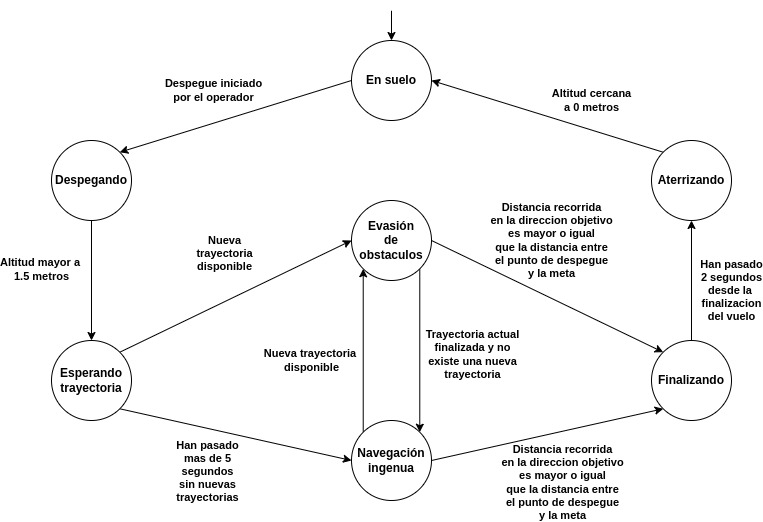
\includegraphics[scale=0.54]{partes/img/State Machine.jpg}
    \caption[Visualización de la máquina de estados que guía la ejecución del hilo principal del ejecutor de trayectorias.]{Visualización de la máquina de estados que guía la ejecución del hilo principal del ejecutor de trayectorias. Los nodos del grafo dirigido representan los estados, sus lados las transiciones y el texto asociado a cada lado representa el predicado de transición.}
    \label{fig:state-machine}
\end{figure}

El estado ``En suelo'' es el estado inicial de la máquina de estados, representa el momento en el que QUAV está en suelo, bien sea porque se esta preparando para despegar o porque acaba de completar un aterrizaje. El estado ``Despegando'' está activo durante el proceso despegue, el proceso de despegue comienza cuando el operador del QUAV inicia la secuencia de despegue, bien sea manualmente o de forma autónoma. Una vez que el vehículo alcanza una altitud de 1.5 metros o mayor, el estado ``Esperando trayectoria'' se activa; este estado espera a que se genere una trayectoria, esto es, que el proceso de inferencia envie el mensaje \texttt{NEW\_TRAJ} y que dicho mensaje se procese por el hilo de nuevas trayectorias, en otras palabras, este estado espera a que \texttt{current\_traj} esté definido. Luego, si pasados cinco segundos aún no se genera una trayectoria, el estado ``Navegación ingenua'' se activa; en caso contrario, el estado ``Evasión de obstáculos'' se activa.

Los estados ``Evasión de obstáculos'' y ``Navegación ingenua'' son los estados más importantes para la ejecución del vuelo evadiendo obstáculos. En resumen, el estado ``Evasión de obstáculos'' ejecuta la trayectoria más reciente generada por el proceso de inferencia y el estado ``Navegación ingenua'' navega directamente en dirección a \jim{\mu_{goal}}, la meta. Recordando que el proceso de inferencia envía nuevas trayectorias siempre y cuando hayan obstáculos a esquivar; el estado ``Evasión de obstáculos'' se activa cuando es necesario evadir un obstáculo y el estado ``Navegación ingenua'' se activa cuando no hay obstáculos cercanos en la dirección objetivo. 

El procedimiento de ejecución del estado ``Navegación ingenua'' es bastante simple, se obtiene la dirección objetivo, se le multiplica \jim{v_{des} = 1} m/s la rapidez de ejecución deseada, y se invoca la función \texttt{sendRefVelocity} del \textit{ACSL Flight API} para que el QUAV navegue directamente en esa dirección. Recordando que \jim{B} es el sistema de referencia del cuerpo del QUAV y \jim{E} es el sistema de referencia inercial; la función \texttt{sendRefVelocity} permite especificar \jim{\omega_{B_z}} la velocidad rotacional alrededor del eje \jim{z} de \jim{B}. Este estado, además de especificar la velocidad, estima la cantidad \jim{\omega_{B_z}} necesaria para que el encabezamiento del QUAV y la dirección objetivo estén en la misma linea. Dicho esto, El pseudo-código del procedimiento de ejecución del estado ``Navegación ingenua'' se muestra en el Algoritmo \ref{alg:naive-execution}.

\begin{algorithm}
\caption{Pseudo-código del procedimiento de ejecución del estado ``Navegación ingenua''. }
\label{alg:naive-execution}
\KwData{\texttt{acslFlightApi}, \texttt{M.shared}, \jim{v_{des}}}

Obtener \texttt{fcu\_state} de \texttt{M.shared}.

Utilizar \texttt{fcu\_state} para obtener \jim{\mu \in \mathbb{R}^{3}}, posición del QUAV en coordenadas NED.

Utilizar \texttt{fcu\_state} para obtener \jim{\mu_{goal} \in \mathbb{R}^{3}}, la posición del objetivo del vuelo en coordenadas NED.

Definir la dirección objetivo como \jim{r_E = \frac{1}{\|\mu_{goal} - \mu\|}(\mu_{goal} - \mu)}.

Estimar la velocidad angular instantánea alrededor del eje \jim{B_z} para alinear el encabezamiento del QUAV con \jim{r_E}, esto es \jim{\omega_{B_z} = \arctan_2(r_{E_y}, r_{E_x}) - \psi } donde \jim{\psi} es el ángulo \textit{yaw} del vehículo.

Utilizar \texttt{fcu\_state} para obtener la matriz de transformación entre \jim{E} y \jim{B}, esto es \jim{R_{E}^{B} = R_{\phi}R_{\theta}R_{\psi}} donde \jim{\phi,\theta,\psi} son los ángulos de Euler de B. 

Obtener la dirección objetivo con respecto a \jim{B}, \jim{r_B = R_{E}^{B} r_E}.

Definir la nueva velocidad, \jim{V_{B} = v_{des} \cdot r_B}

$\text{\texttt{acslFlightApi.sendRefVelocity(}}V_{B}, \omega_{B_z}\text{\texttt{)}}$

\end{algorithm}

\pagebreak

Por otro lado, el procedimiento de ejecución del estado ``Evasión de obstáculos'' evalúa la proyección polinómica de la trayectoria actual \texttt{current\_traj} para obtener la velocidad instantánea, posteriormente invoca \texttt{sendRefVelocity} para enviar la referencia de la velocidad y de \jim{\omega_{B_z}} al FCU. Si \texttt{traj\_mutex} es el semáforo de exclusión mutua para el acceso a \texttt{current\_traj}, el pseudo-código del procedimiento de ejecución del estado ``Evasión de obstáculos'' se muestra en el Algoritmo \ref{alg:traj-execution}.

\begin{algorithm}
\caption{Pseudo-código del procedimiento de ejecución del estado ``Evasión de obstáculos''. }
\label{alg:traj-execution}
\KwData{\texttt{acslFlightApi}, \texttt{M.shared}, \texttt{current\_traj}, \texttt{traj\_mutex}}

Obtener el tiempo actual del sistema \jim{t_{now}} en segundos.

\texttt{traj\_mutex.incrementar()}

Obtener \jim{t_{ref}} de \texttt{current\_traj} en segundos.

$dt = t_{now} - t_{ref}$

\If{$dt > 1$}{
    Trayectoria completada, \texttt{traj\_mutex.decrementar()} y \Return
}

Obtener $a_x, a_y$ los coeficientes de la proyección polinómica de \texttt{current\_traj} para los ejes \jim{x,y} respectivamente.

$T^\prime = [0, 1, 2dt, 3dt^2]$

$v_x = a_{x}^T \cdot T^\prime$

$v_y = a_{y}^T \cdot T^\prime$

\texttt{traj\_mutex.decrementar()}

Por motivos de validación de concepto, se limita la ejecución de las trayectorias inferidas al plano \jim{B_xB_y}, esto es \jim{v_z = 0}.

$V_{B} = [v_x, v_y, v_z]^T$

Obtener \texttt{fcu\_state} de \texttt{M.shared}.

Utilizar \texttt{fcu\_state} para obtener la matriz de transformación entre \jim{B} y \jim{E}, esto es \jim{R_{B}^{E} = (R_{E}^{B})^T = (R_{\phi}R_{\theta}R_{\psi})^T} donde \jim{\phi,\theta,\psi} son los ángulos de Euler de B. 

$V_{E} = R_{B}^{E} V_{B}$

Estimar la velocidad angular instantánea alrededor del eje \jim{B_z} para que el encabezamiento del QUAV apunte hacia la dirección tangencial de la trayectoria, esto es \jim{\omega_{B_z} = \arctan_2(V_{E_y}, V_{E_x}) - \psi } donde \jim{\psi} es el ángulo \textit{yaw} del vehículo.

$\text{\texttt{acslFlightApi.sendRefVelocity(}}V_{B}, \omega_{B_z}\text{\texttt{)}}$

\end{algorithm}

Tanto el estado ``Navegación ingenua'' como el estado ``Evasión de obstáculos'' tienen una transición al estado ``Finalizando'', esta transición se cumple cuando cuando la distancia recorrida en la dirección objetivo es mayor o igual que la distancia entre el punto de despegue y la meta; esta condición se utilizó para preferir que el QUAV aterrice si la evasión de obstáculos lo desvió considerablemente de camino original, así como también para que se aterrice una vez que se alcanzó la meta. Dependiendo de la configuración de los obstáculos, es posible que no sea posible avanzar hacia la meta sin desviarse considerablemente, esta transición se asegura de que en ese caso se aterrice el vehículo y se termine el vuelo. En términos formales, trabajando en el sistema de coordenadas NED, si \jim{\mu_0} es posición del QUAV después del despegue y antes de comenzar la navegación; \jim{\mu} es la posición actual del QUAV; y \jim{\mu_{goal}} es la posición de la meta. Esta transición se cumple si la expresión de la Ecuación \ref{eq:finishing-condition} se evalúa a verdadero.

\begin{equation}
    \label{eq:finishing-condition}
    (\mu - \mu_0)^T \cdot \left (\frac{\mu_{goal} - \mu_0}{\|\mu_{goal} - \mu_0\|}  \right) \geq \|\mu_{goal} - \mu_0\|
\end{equation}

El estado ``Aterrizando'' se activa una vez que han pasado dos segundos desde que activó el estado ``Finalizando'', este estado invoca al método \texttt{land} del \textit{ACSL Flight API} para ordenar al FCU que aterrice el QUAV de forma autónoma. Una vez que la altitud es cercana a cero metros, se activa una vez más el estado ``En suelo'' y la ejecución finaliza.

Es importante mencionar que esta máquina de estados fue diseñada para el caso donde se hace un solo vuelo, en donde el objetivo se encuentra a distancia predefinida en la dirección del encabezado del QUAV al momento del despegue. Para aplicaciones donde exista una secuencia de puntos objetivos sera necesario utilizar una variante de esta máquina de estados en donde se tome en cuenta la secuencia de vuelo. 

\section{Ajuste fino de la política estudiante}

\label{sec:imp-finetune}

Para que las trayectorias generadas por el proceso de inferencia cumplan con la restricción de poder ejecutarse a una rapidez promedio de \jim{v_{des} = 1} m/s; es necesario realizar un ajuste de los pesos de la red neuronal publicada por \cite{Loquercio2021}. Los pesos que se descargaron del repositorio de \textit{Learning High Speed Flight in the Wild} fueron entrenados con una base de datos de trayectorias con \jim{v_{des} = 7} m/s. Por lo tanto, siguiendo las recomendaciones de los autores de \cite{Loquercio2021}, para obtener una política estudiante que sea capaz de evadir obstáculos a una velocidad considerablemente inferior, es necesario realizar un proceso de ajuste fino de los pesos provistos. Según las recomendaciones de uso del método propuesto en \cite{Loquercio2021}, entrenar una política estudiante requiere de una base de datos extensa de trayectorias generadas por el experto privilegiado, esto acompañado de un tiempo de entrenamiento considerable; es por esto que en su lugar, recomiendan ajustar los pesos de la política estudiante que ejecuta con \jim{v_{des} = 7} m/s en lugar de entrenar desde cero.

Para realizar este ajuste fino, se utilizó la plataforma de generación de base de datos del experto informado publicada en el repositorio de \cite{Loquercio2021}. Luego de ajustar la velocidad de ejecución del experto a \jim{v_{des} = 1} m/s, se procedió a generar una base de datos de trayectorias libres de colisión dentro del entorno de ``bosque denso'', que justamente es el entorno principal utilizado en el trabajo original \cite{Loquercio2021} y que consiste en un bosque con árboles cuya posición se determina por una distribución aleatoria de \textit{Poisson} \cite{Loquercio2021}. Se realizaron 193 simulaciones, cada una generando entre 300 y 350 ejemplos. De esas 193 simulaciones, se tomaron 168 para formar una base de datos de entrenamiento y 25 para una base datos de validación; en otras palabras, se particionó la base de datos en \jim{~88\%} conjunto de entrenamiento y \jim{~12\%} conjunto de validación.

Se realizó entrenamiento supervisado con la base de datos generada por un total de 33 épocas; comenzando desde la época en el que se encontraba el punto de control de los pesos publicados por \cite{Loquercio2021}, la época número  188; hasta la época número  221. Por limitaciones de memoria del computador de entrenamiento, el valor del tamaño del \textit{batch} se redujo de 8 a 1. El valor del resto de los los hiper-parámetros del entrenamiento fueron los mismos utilizados por \cite{Loquercio2021} para la época 188.

\section{Resumen}

En este capítulo se detalla la implementación de la solución propuesta para abordar el problema de evasión de obstáculos en el contexto de los QUAVs. Comienza presentando la metodología y la plataforma de implementación en la Sección \ref{sec:imp-platform}, destacando la infraestructura utilizada para desarrollar y evaluar la solución. En la Sección \ref{sec:imp-algo}, se justifica la elección del algoritmo de evasión de obstáculos, basándose en el enfoque presentado en \textit{Learning high-speed flight in the wild} \cite{Loquercio2021}.

La Sección \ref{sec:imp-arch} se dedica a la descripción detallada de la arquitectura de la solución propuesta, incluyendo el funcionamiento de cada uno de sus componentes. Allí se profundiza en los aspectos cruciales de la ejecución de la solución, en donde destacan el funcionamiento del proceso de inferencia y del ejecutor de trayectorias. Finalmente, en la Sección \ref{sec:imp-finetune}, se explora el proceso de refinamiento fino de la red neuronal encargada de la inferencia de trayectorias libre de colisión, es decir, el perfeccionamiento de la política estudiante.

El trabajo desarrollado en este capítulo representa el núcleo del proyecto. Especialmente hay que destacar el logro de implementar una solución que permite a un QUAV evadir obstáculos de forma autónoma y sin información previa del entorno, que además puede ejecutarse en tiempo real sobre un hardware ligero y con recursos limitados. Sin mencionar que la totalidad de la solución trabaja en concordancia y sobre el marco de trabajo de ACSL, permitiendo una integración automática con el ecosistema de aplicaciones de los vehículos de ACSL.

En general, este capítulo sienta las bases para la evaluación del desempeño de la solución propuesta, que se abordará en el próximo capítulo. El análisis detallado de la implementación proporciona una comprensión completa de la estructura y funcionamiento de la solución, preparando el terreno para la discusión de resultados y conclusiones.
\chapter{Resultados}
\label{capitulo6}
\lhead{Capítulo 6. \emph{Resultados}}

En el capítulo anterior, se detalló la implementación de la solución propuesta para abordar el problema de evasión de obstáculos en QUAVs, centrándose en la metodología, la plataforma de implementación, la justificación del algoritmo seleccionado y la descripción del funcionamiento de los componentes principales. Este capítulo se adentra ahora en la evaluación y presentación de los resultados obtenidos, proporcionando una perspectiva crítica sobre el rendimiento de la solución propuesta.

En la Sección  \ref{sec:results-finetune} se examinan los resultados del ajuste fino de la política estudiante, destacando los desafíos asociados al sobre-ajuste de los datos de entrenamiento y a la generación de la base de datos. Además, se exploran las consecuencias derivadas de estos problemas al evaluar la política de evasión de obstáculos.

La Sección  \ref{sec:results-flights} examina los resultados de la política de evasión de obstáculos, dividida en dos subsecciones clave: la Sección  \ref{sec:results-AirSim}, que presenta los resultados de vuelos en simulación, y la Sección  \ref{sec:results-SOTEN}, centrada en vuelos sobre la plataforma física de implementación, SOTEN. Estos resultados ofrecen una perspectiva del rendimiento de la solución en configuraciones simples de obstáculos, cuya política de evasión se muestra estable. Además, se evalúan otras configuraciones de obstáculos en donde la política no logra completar su función de manera satisfactoria, y se identifica la relación entre este resultado y los desafíos asociados al ajuste fino de la política estudiante.

El análisis detallado de estos resultados proporciona una evaluación crítica de la efectividad de la solución propuesta, sirviendo como base para la discusión en el siguiente capítulo. Aquí, se extraerán conclusiones significativas y se identificarán posibles direcciones para mejorar el rendimiento en futuras investigaciones en el campo de evasión de obstáculos en QUAVs.

\section{Resultados del ajuste fino de la política estudiante}

\label{sec:results-finetune}

Como se menciona en el capítulo anterior, el objetivo del ajuste fino de la política estudiante, es ajustar los pesos provistos por los autores del trabajo original \cite{Loquercio2021} para que la red neuronal genere trayectorias con \jim{v_{des} = 1} m/s; idealmente, manteniendo un nivel de generalización comparable a la red publicada en \cite{Loquercio2021}. Recordando que la función de pérdida de la red neuronal de la política estudiante tiene dos componentes: un componente espacial que cuantifica qué tan cerca se encuentran las trayectorias predichas a las generadas por el experto, y un componente de estimación que cuantifica qué tan correctamente se hace la estimación del costo de ejecución \jim{c_k} \cite{Loquercio2021}; la Figura \ref{fig:loss-space-all} y la Figura \ref{fig:loss-estim-all} muestran el valor del componente espacial y de estimación en función de las épocas, tanto para el conjunto de entrenamiento como para el de validación.

\begin{figure}[H]
    \centering
    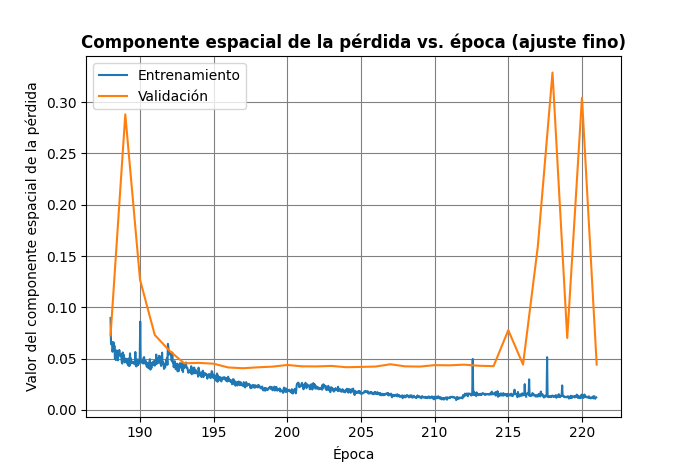
\includegraphics[scale=0.6]{partes/img/loss-space-all.png}
    \caption[Componente espacial de la pérdida vs. época (ajuste fino).]{Componente espacial de la pérdida vs. época (ajuste fino). Se observa claramente la divergencia de la pérdida sobre el conjunto de validación a partir de la época 215.}
    \label{fig:loss-space-all}
\end{figure}

\begin{figure}[H]
    \centering
    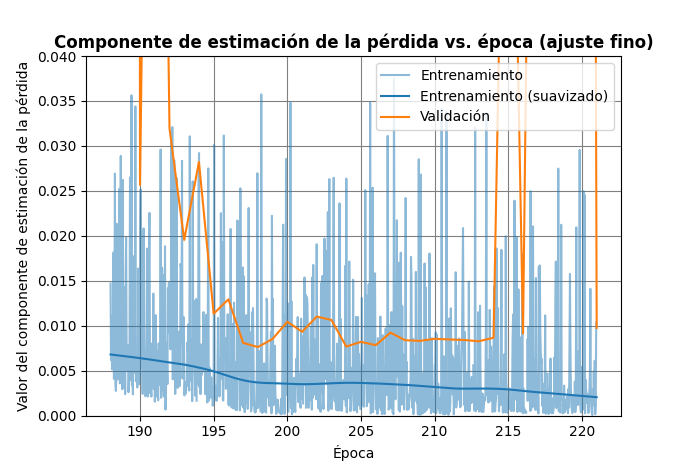
\includegraphics[scale=0.6]{partes/img/loss-estim-all.png}
    \caption[Componente de estimación de la pérdida vs. época (ajuste fino).]{Componente de estimación de la pérdida vs. época (ajuste fino). Se observa claramente la divergencia de la pérdida sobre el conjunto de validación a partir de la época 215.}
    \label{fig:loss-estim-all}
\end{figure}

La Figura \ref{fig:loss-space-all} y la Figura \ref{fig:loss-estim-all} reflejan la divergencia del valor de la pérdida sobre el conjunto de validación a partir de la época 215. Para contrarrestar este efecto, se decidió utilizar un punto de control temprano antes de la divergencia, efectivamente deteniendo el entrenamiento de forma temprana. El punto de control más cercano anterior a la época 215 fue el punto de control de la época 213. Al regresar a dicho punto de control se eliminó la divergencia del valor de pérdida de validación. La Figura \ref{fig:loss-space-stopped} y la Figura \ref{fig:loss-estim-stopped} muestran el valor del componente espacial y de estimación en función de las épocas luego de detener tempranamente el entrenamiento, tanto para el conjunto de entrenamiento como para el de validación. 

\begin{figure}[H]
    \centering
    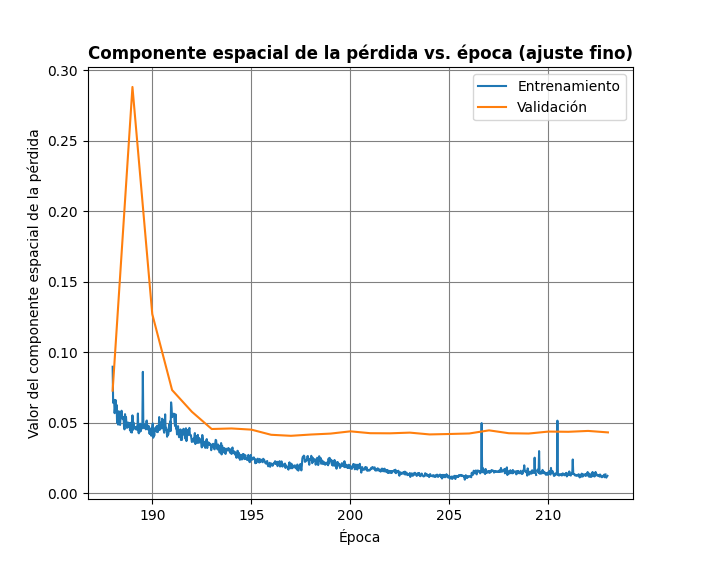
\includegraphics[scale=0.6]{partes/img/loss-space-stopped.png}
    \caption[Componente espacial de la pérdida vs. época (ajuste fino) luego de detener el entrenamiento tempranamente.]{Componente espacial de la pérdida vs. época (ajuste fino) luego de detener el entrenamiento tempranamente. No se observa divergencia en el valor de la pérdida sobre el conjunto de validación.}
    \label{fig:loss-space-stopped}
\end{figure}

\begin{figure}[H]
    \centering
    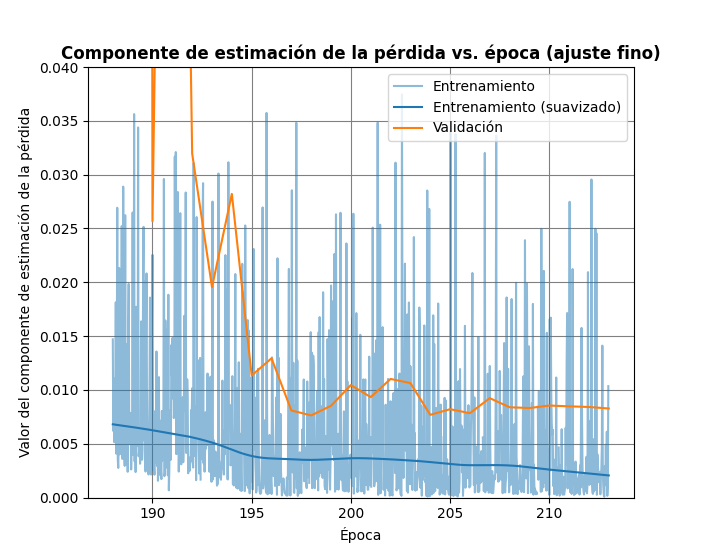
\includegraphics[scale=0.6]{partes/img/loss-estim-stopped.png}
    \caption[Componente de estimación de la pérdida vs. época (ajuste fino) luego de detener el entrenamiento tempranamente.]{Componente de estimación de la pérdida vs. época (ajuste fino) luego de detener el entrenamiento tempranamente. No se observa divergencia en el valor de la pérdida sobre el conjunto de validación.}
    \label{fig:loss-estim-stopped}
\end{figure}

Luego de eliminar la divergencia de la pérdida de validación, se puede proceder a evaluar este modelo contra el modelo original. Como las métricas de utilizadas en la evaluación del método propuesto en \cite{Loquercio2021} evalúan el sistema completo, la única métrica que se puede utilizar para comparar modelos es, exclusivamente, el valor de la función de pérdida a lo largo de un conjunto de datos. Para que esta comparación sea efectiva, lo importante es seleccionar conjuntos de datos representativos de la comparación deseada. Precisamente esto es lo que se utilizó en este trabajo como herramienta de comparación del desempeño de los modelos de interés. El procedimiento y resultados de la evaluación se describe a continuación.

Los modelos a comparar son el modelo original, que destaca en la capacidad de predecir trayectorias sin colisión con \jim{v_{des} = 7} m/s; y el modelo ajustado en este trabajo para predecir trayectorias sin colisión con \jim{v_{des} = 1} m/s. Para ello, se seleccionaron dos conjuntos de datos, el conjunto de datos de validación con trayectorias con \jim{v_{des} = 7} m/s (utilizado en el entrenamiento del modelo original) y el conjunto de datos de validación con las trayectorias con \jim{v_{des} = 1} m/s (el generado en el presente trabajo). La diferencia en los valores de pérdida entre esos modelos y conjuntos de datos, dan una idea del rendimiento relativo de cada uno de los modelos dentro de los escenarios presenciados en el conjunto de datos. La Tabla \ref{table:loss-comparison} compara los valores de pérdida de cada modelo sobre cada conjunto de datos de interés.

\begin{table}[h]
    \centering
    \begin{tabular}{||c | c || c | c ||} 
     \hline
     \textbf{Modelo} & \textbf{Conjunto de datos} & \jim{L_{esp}} & \jim{L_{est}}  \rule{0pt}{2.6ex} \\ [0.4ex] 
     \hline\hline
     Original & Original a 7 m/s & \textbf{1.407} & 0.1069 \\ 
     \hline
     Original & Generado a 1 m/s & \textbf{41.7108} & 0.0842 \\ 
     \hline
     Ajustado & Generado a 1 m/s & \textbf{0.0441}  & 0.0008 \\
     \hline
    \end{tabular}
    \caption[Comparación de los valores de pérdida entre modelo original y ajustado según el conjunto de datos evaluado.]{Comparación de los valores de pérdida entre modelo original y ajustado según el conjunto de datos evaluado. \jim{L_{esp}} es el valor del componente espacial de la pérdida y \jim{L_{est}} es el valor del componente de estimación de la pérdida.}
    \label{table:loss-comparison}
\end{table}

De esta comparación podemos se pueden realizar algunas observaciones relevantes. Primero, el modelo original tiene dificultades en generar trayectorias con las características espaciales de las trayectorias con \jim{v_{des} = 1} m/s, esto tiene sentido pues la diferencia espacial entre moverse a 7 m/s y 1 m/s es bastante alta; esto simplemente confirma la dependencia entre \jim{v_{des}} del experto y el desempeño de la política estudiante a distintas velocidades, tal como se afirma en \cite{Loquercio2021}. Por otro lado, el modelo original logra generalizar la tarea de estimar el costo de ejecución de una trayectoria, los valores del componente de estimación de la pérdida están en el mismo orden tanto para \jim{v_{des} = 7} m/s como para \jim{v_{des} = 1} m/s. 

Segundo, y más relevante para este trabajo, los valores de pérdida del modelo ajustado sobre el conjunto con \jim{v_{des} = 1} m/s, están dos órdenes de magnitud por debajo de los valores del modelo original sobre el conjunto con \jim{v_{des} = 7} m/s; esto puede indicar la presencia de sobre-ajuste (pérdida de capacidad de generalización), sin embargo, este sobre-ajuste no existe al nivel de conjuntos de entrenamiento y de validación, sino que existe al nivel de los conjuntos de datos generados por el experto con distintos valores de \jim{v_{des}}. Para confirmar esta línea de pensamiento, se procede a visualizar una muestra de las trayectorias generadas con \jim{v_{des} = 1} m/s y compararlas con una muestra de las trayectorias generadas con \jim{v_{des} = 7} m/s. Si ambos conjuntos de datos tienen niveles equivalentes de generalización, se debería observar en cada muestra una representación amplia de distintas trayectorias. Si alguna de las dos muestras tiene preferencia por un caso particular de trayectorias con respecto a la otra muestra, entonces esa base de datos tiene menos capacidad de generalización relativamente. De cada base de datos se seleccionaron tres vuelos aleatoriamente, la Figura \ref{fig:7ms-sample} y la Figura \ref{fig:1ms-sample} visualizan las muestras seleccionadas. Cada muestra se visualiza como una vista ``de arriba hacia abajo'' de la nube de puntos del entorno junto con las trayectorias generadas durante el vuelo; el color de las trayectorias interpola entre azul y rojo, mientras más rojo, más costo de ejecución tiene la trayectoria. Este experimento se repitió 10 veces con resultados similares. Para facilitar la visualización de los resultados, solo se muestra un solo experimento.

\begin{figure}[H]
    \centering
    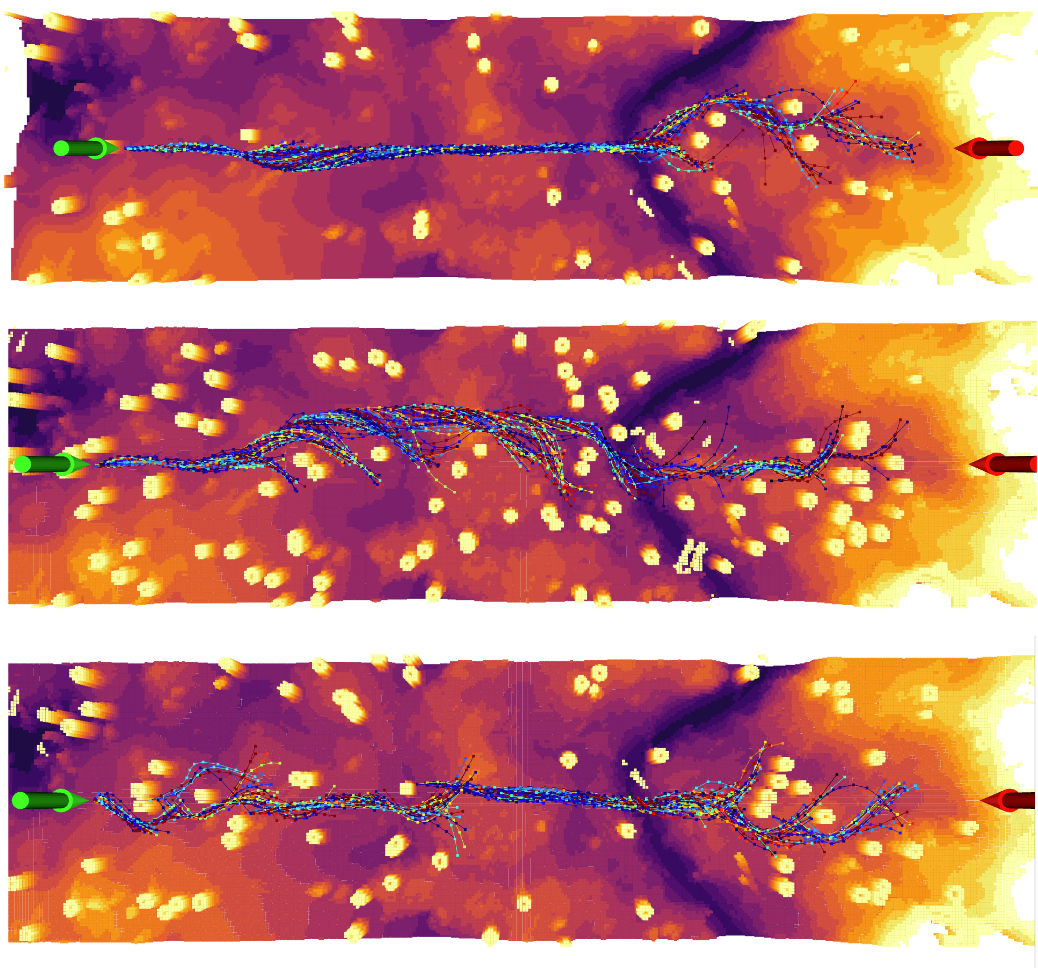
\includegraphics[scale=0.4]{partes/img/7ms-sample.png}
    \caption[Visualización de tres vuelos de la base de datos con \jim{v_{des} = 7} m/s.]{Visualización de tres vuelos de la base de datos con \jim{v_{des} = 7} m/s.}
    \label{fig:7ms-sample}
\end{figure}

\begin{figure}[H]
    \centering
    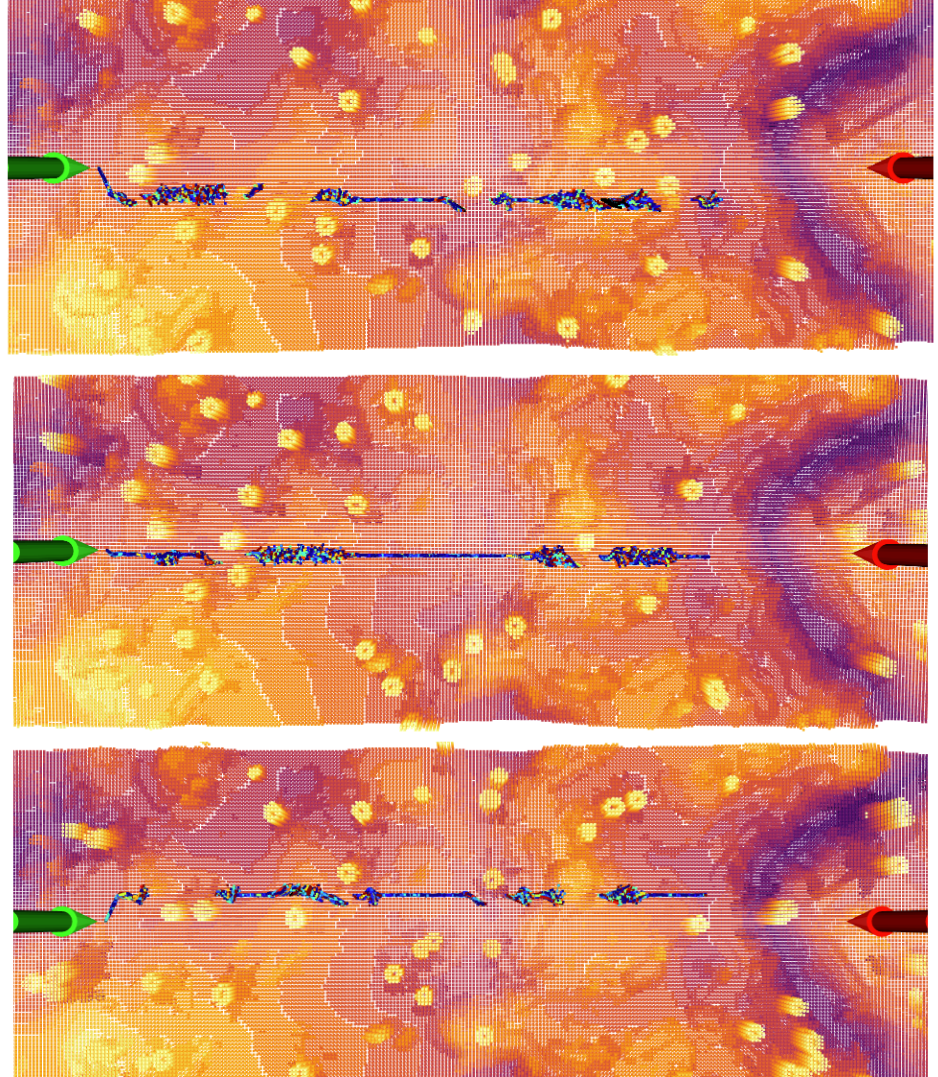
\includegraphics[scale=0.4]{partes/img/1ms-sample.png}
    \caption[Visualización de tres vuelos de la base de datos con \jim{v_{des} = 1} m/s.]{Visualización de tres vuelos de la base de datos con \jim{v_{des} = 1} m/s.}
    \label{fig:1ms-sample}
\end{figure}

A simple vista se observa una clara diferencia, en la base de datos con \jim{v_{des} = 1} m/s, los obstáculos solo se esquivan por uno solo de los flancos del obstáculo, mientras en la base de datos con \jim{v_{des} = 7} m/s se exploran ambos flancos como posibilidades de esquivar el obstáculo. Para cuantificar esta observación, se procedió a contar para cada conjunto de datos, el porcentaje de ejemplos en donde la trayectoria se dirige hacia la izquierda, hacia la derecha y hacia al frente. Para determinar si un ejemplo de la base de datos va hacia a la izquierda, derecha o hacia el frente; se calculan \jim{D_{r}} y \jim{D_{l}} los desplazamientos máximos hacia la derecha y hacia la izquierda respectivamente, con respecto al marco de referencia del cuerpo del QUAV. Luego si \jim{\vert D_{r} - D_{l}\vert < 0.1 } se considera que la trayectoria va hacia el frente, si \jim{D_{r} > D_{l}} se considera que la trayectoria va hacia la derecha y si \jim{D_{r} < D_{l}} se considera que la trayectoria va hacia la izquierda. Solo se consideran los ejemplos en donde exista un obstáculo visible a 5m de distancia. La Tabla \ref{table:flank-count} muestra los resultados de este conteo. 

\begin{table}[h]
    \centering
    \begin{tabular}{||c | c | c | c | c ||} 
     \hline
     \textbf{Conjunto de datos} & \jim{P_{left}} & \jim{P_{right}} & \jim{P_{str}} & \jim{N_{samples}} \rule{0pt}{2.6ex} \\ [0.4ex] 
     \hline\hline
     \jim{v_{des} = 7} m/s & 51.3\% & 44.1\% & 4.5\% & 5517 \\ 
     \hline
     \jim{v_{des} = 1} m/s & 40.6\% & 35.1\% & 24.3\% & 18244 \\ 
     \hline
    \end{tabular}
    \caption[Distribución de ejemplos en cada conjunto de datos según hacia donde se dirige la trayectoria.]{Distribución de ejemplos en cada conjunto de datos según hacia donde se dirige la trayectoria. \jim{P_{left}} es el porcentaje de ejemplos en donde la trayectoria se dirige hacia la izquierda, \jim{P_{right}} es el porcentaje de ejemplos en donde la trayectoria se dirige hacia la derecha, \jim{P_{str}} es el porcentaje de ejemplos en donde la trayectoria se dirige hacia el frente y \jim{N_{samples}} es el número de ejemplos en el conjunto de datos.}
    \label{table:flank-count}
\end{table}

De los resultados presentados en la Tabla \ref{table:flank-count} podemos realizar varias observaciones. Primero ambos conjuntos de datos tienen un desbalance entre \jim{P_{left}} y \jim{P_{right}}, con \jim{P_{left}} dominando por 5\%. Segundo, el conjunto de datos con \jim{v_{des} = 1} m/s contiene un número mucho mayor de trayectorias que se dirigen hacia el frente, con un 24.3\% de los ejemplos, mientras que el conjunto de datos con \jim{v_{des} = 7} m/s solo tiene un 4.5\% de los ejemplos. Tercero, el conjunto de datos con \jim{v_{des} = 1} m/s tiene un 230\% más ejemplos que el conjunto de datos con \jim{v_{des} = 7} m/s, esto probablemente como consecuencia de recorrer una distancia menor en promedio por trayectoria (por la menor rapidez de desplazamiento). 

Como la decisión de esquivar un obstáculo en el plano \jim{xy} se reduce a esquivar por el flanco izquierdo o por el flanco derecho del obstáculo (pues seguir hacia el frente implica colisión), el desbalance entre \jim{P_{left}} y \jim{P_{right}} es el factor mas relevante en la diferencia de capacidad de generalización entre los conjuntos de datos. Este factor es además acentuado en el conjunto con \jim{v_{des} = 1} m/s por el mayor número de ejemplos que se dirigen hacia el frente, y por el mayor número de ejemplos en general; haciendo que el 5\% de desbalance entre \jim{P_{left}} y \jim{P_{right}} sea mucho más relevante. Es por esto que el modelo ajustado va a tener una preferencia a esquivar obstáculos por el flanco izquierdo. En otras palabras, existe un desbalance de las modas de la distribución \jim{P}\footnote{La distribución \jim{P} se describe en la Ecuación \ref{eq:aoa-expert-P}} en la base de datos con \jim{v_{des} = 1} m/s que no existe significativamente en en la base de datos con \jim{v_{des} = 7} m/s. Este desbalance hace que el proceso de refinamiento fino produzca un efecto de sobre-ajuste con respecto al rendimiento de la política publicada en \cite{Loquercio2021}. El modelo se ajusta demasiado a los ejemplos de la base datos con \jim{v_{des} = 1} m/s, en donde existe una preferencia significativa a esquivar obstáculos por el flanco izquierdo, potencialmente reduciendo su capacidad multi-modal al momento de generar trayectorias.

Un posible origen de este problema, es que la poca longitud de las trayectorias generadas para \jim{v_{des} = 1} m/s no permite que el experto genere trayectorias que consideren todas las modas de la distribución \jim{P} con un valor de costo bajo. Cuando el experto selecciona las mejores tres trayectorias, algunas de las trayectorias que consideran las modas de \jim{P} se descartan, produciendo el desbalance. Otra posible razón puede ser que el planificador de trayectorias globales que genera \jim{\tau_{ref}} no permita la exploración de dichas trayectorias, principalmente por planificar trayectorias triviales en donde se navegue mayoritariamente sin encontrar obstáculos. 

Una posible solución para este problema es modificar el entorno de simulación para que la configuración de los obstáculos permita que el experto considere las modas de \jim{P} con alto valor de costo, por ejemplo, incrementando la densidad de los obstáculos y reduciendo sus dimensiones. Otra posible solución es modificar los parámetros del planificador de trayectorias globales de forma que la ejecución de \jim{\tau_{ref}} fomente la exploración de obstáculos en donde se generen muestras que representen el carácter multi-modal de \jim{P}, por ejemplo, intencionalmente dirigiéndose hacia la cercanía de grupos de obstáculos. Alternativamente se pueden ejecutar las predicciones de la red en lugar de seguir una \jim{\tau_{ref}} planificada globalmente, y en su lugar utilizar una \jim{\tau_{ref}} que simplemente sea el camino en línea recta desde el punto de despegue hasta la meta; esto potencialmente va a incrementar la exploración de obstáculos en donde se generen muestras que representen múltiples modas de \jim{P}.

Dicho esto, por limitaciones del tiempo de desarrollo, y recomendaciones por parte del equipo de ACSL, en este trabajo no se soluciona el problema descrito anteriormente. Esto significa que la política estudiante utilizada en este trabajo sufre las consecuencias del sobre-ajuste ocasionado por el desbalance de modas en la base de datos con \jim{v_{des} = 1} m/s, esto puede ocasionar que la política de evasión de obstáculos tenga una preferencia fuerte en esquivar obstáculos de una forma en particular. En las siguientes secciones se observa que efectivamente, la política de evasión de obstáculos tiene una fuerte preferencia a esquivar obstáculos por el flanco izquierdo, así como también, que este comportamiento hace que la ejecución en entornos no triviales termine en potenciales colisiones.

\section{Resultados de la política de evasión de obstáculos}

\label{sec:results-flights}

\subsection{Vuelos en entorno simulación}

\label{sec:results-AirSim}

En esta sección se describen las configuraciones de los vuelos realizados en el entorno de simulación AirSim \cite{shah2018airsim}, así como también sus resultados y comportamientos observados. Es importante recordar que por motivos de validación del concepto por parte de ACSL, la ejecución de la evasión de obstáculos está limitada al plano \jim{xy} del marco de referencia del cuerpo del QUAV.

La primera configuración de obstáculos utilizada es una configuración simple con un solo obstáculo en la línea directa de visión del QUAV, un diagrama de la configuración se muestra en la Figura \ref{fig:config-1-single}. En el diagrama se muestran dos vistas, la frontal (plano \jim{yz}) a partir desde el punto de despegue y la vista de arriba hacia abajo (plano \jim{xy}).

\begin{figure}[H]
    \centering
    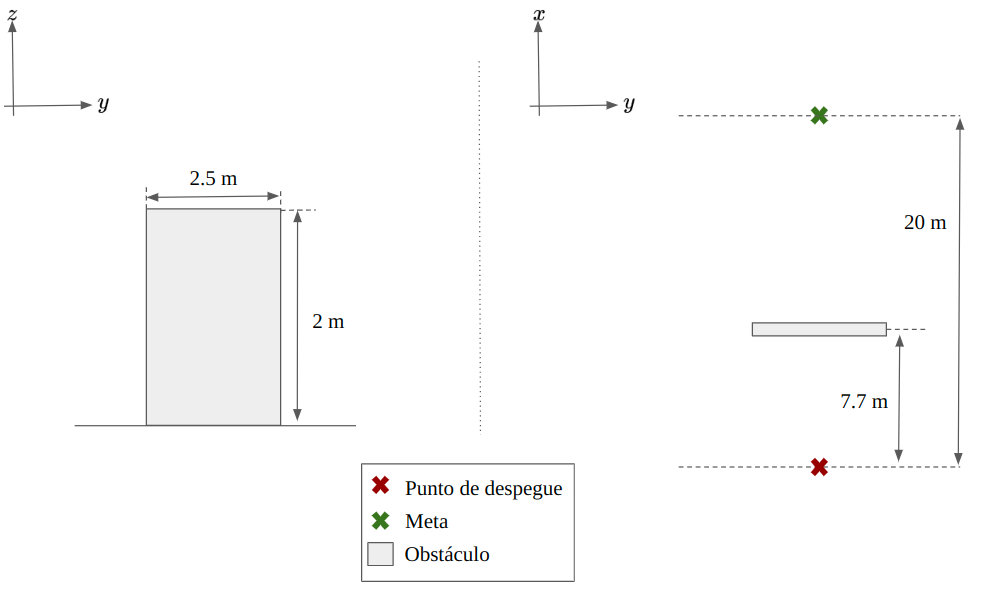
\includegraphics[scale=0.35]{partes/img/config-1-single.png}
    \caption[Primera configuración de obstáculos dentro del entorno de AirSim.]{Primera configuración de obstáculos dentro del entorno de AirSim. Obstáculo simple.}
    \label{fig:config-1-single}
\end{figure}

El comportamiento del algoritmo se mostró capaz de evadir el obstáculo de forma robusta, en concreto, de 10 vuelos ejecutados, 10 resultaron en vuelos sin colisión. La Figura \ref{fig:single-graph-4} muestra una visualización desde arriba hacia abajo de los caminos resultantes de seguir las trayectorias generadas por el algoritmo para cuatro vuelos. Todos los vuelos realizados en esta configuración muestran un comportamiento similar a lo que se observa en la Figura \ref{fig:single-graph-4}, esto es, esquivar el obstáculo hacia la dirección \jim{-y_B}\footnote[1]{Donde \jim{B} es el marco de referencia del cuerpo del QUAV.} y dirigirse hacia la meta una vez no es visible el obstáculo.

\begin{figure}[H]
    \centering
    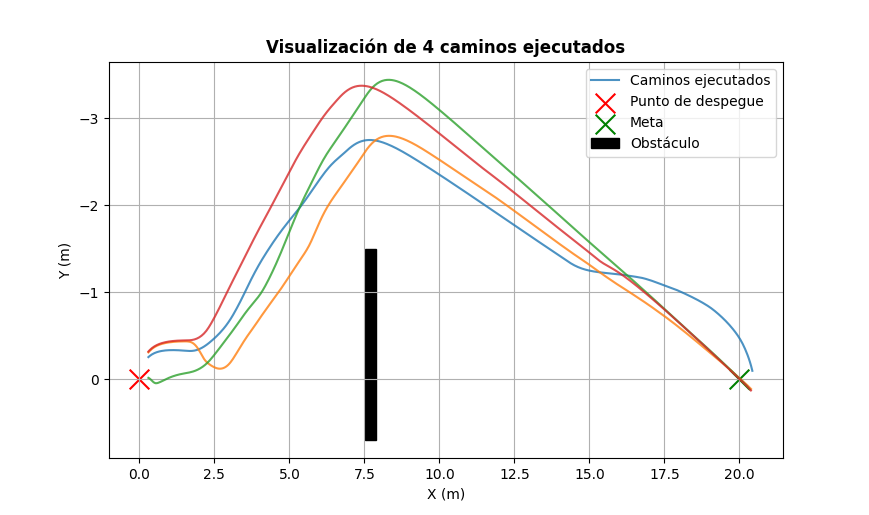
\includegraphics[scale=0.65]{partes/img/sim-single-panel-graph-4.png}
    \caption[Visualización simultánea de cuatro caminos ejecutados dentro de la primera configuración de obstáculos en entorno de simulación.]{Visualización simultánea de cuatro caminos ejecutados dentro de la primera configuración de obstáculos en entorno de simulación. De 10 vuelos ejecutados dentro de esta configuración, 10 resultaron sin colisión.}
    \label{fig:single-graph-4}
\end{figure}

La diferencia más marcada entre vuelos en esta configuración es la desviación máxima del camino ejecutado con respecto al camino directo entre el punto de despegue y la meta, la Figura \ref{fig:single-max-deviation} muestra un diagrama de caja de la desviación máxima de los caminos ejecutados en esta configuración. La desviación máxima promedio de los caminos ejecutados en esta configuración es cerca de 3.1 metros, con una desviación máxima de cerca de 3.45 metros y una desviación mínima de cerca de 2.75 metros.

\begin{figure}[H]
    \centering
    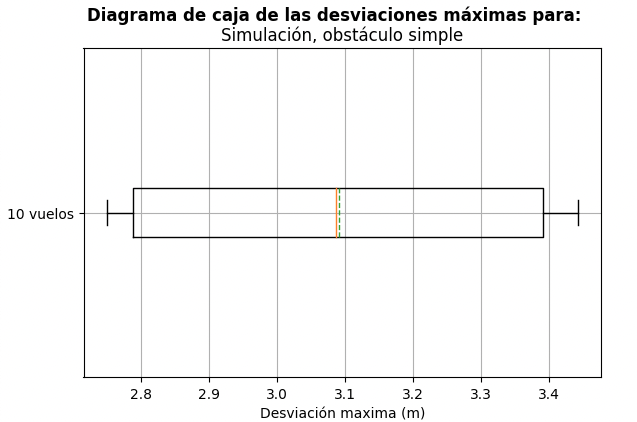
\includegraphics[scale=0.55]{partes/img/sim-single-panel-box.png}
    \caption[Diagrama de caja de la desviación máxima de los caminos ejecutados en la primera configuración de obstáculos en entorno de simulación.]{Diagrama de caja de la desviación máxima de los caminos ejecutados en la primera configuración de obstáculos en entorno de simulación.}
    \label{fig:single-max-deviation}
\end{figure}

La siguiente configuración utilizada es una configuración similar a la anterior pero con un obstáculo adicional también en la misma línea de visión del QUAV. La Figura \ref{fig:config-2-double} muestra el diagrama de la segunda configuración.

\begin{figure}[H]
    \centering
    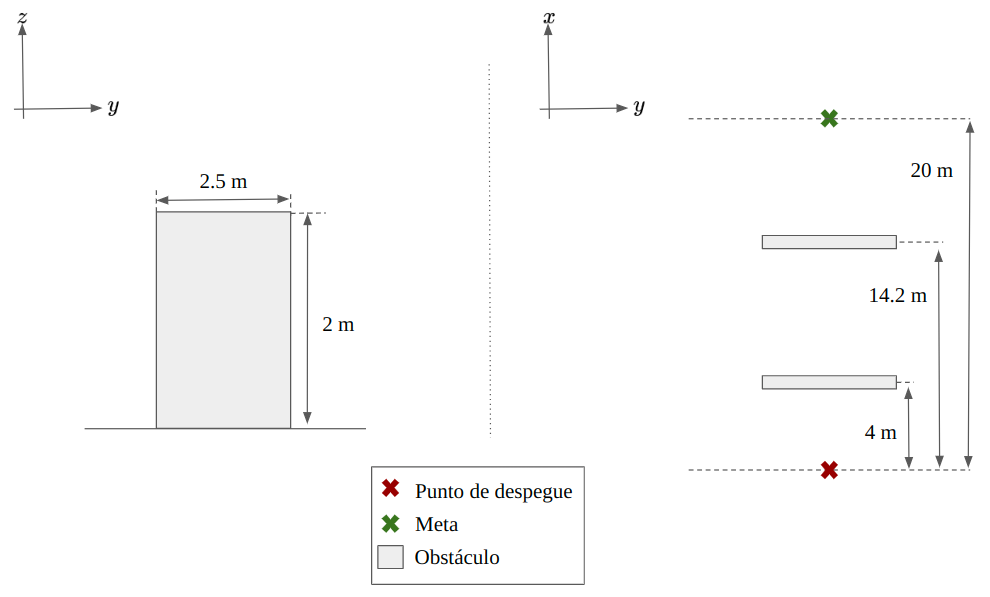
\includegraphics[scale=0.35]{partes/img/config-2-double.png}
    \caption[Segunda configuración de obstáculos dentro del entorno de AirSim.]{Segunda configuración de obstáculos dentro del entorno de AirSim. Dos obstáculos consecutivos en la línea de visión del QUAV.}
    \label{fig:config-2-double}
\end{figure}

Tal como en la configuración anterior, el comportamiento de algoritmo fue estable, de 10 vuelos ejecutados, 10 resultaron en vuelos sin colisión. La Figura \ref{fig:double-graph-4} muestra una visualización desde arriba hacia abajo de caminos resultantes de seguir las trayectorias generadas por el algoritmo para cuatro vuelos. Todos los vuelos realizados en esta configuración muestran un comportamiento similar a lo que se observa en la Figura \ref{fig:double-graph-4}.

\begin{figure}[H]
    \centering
    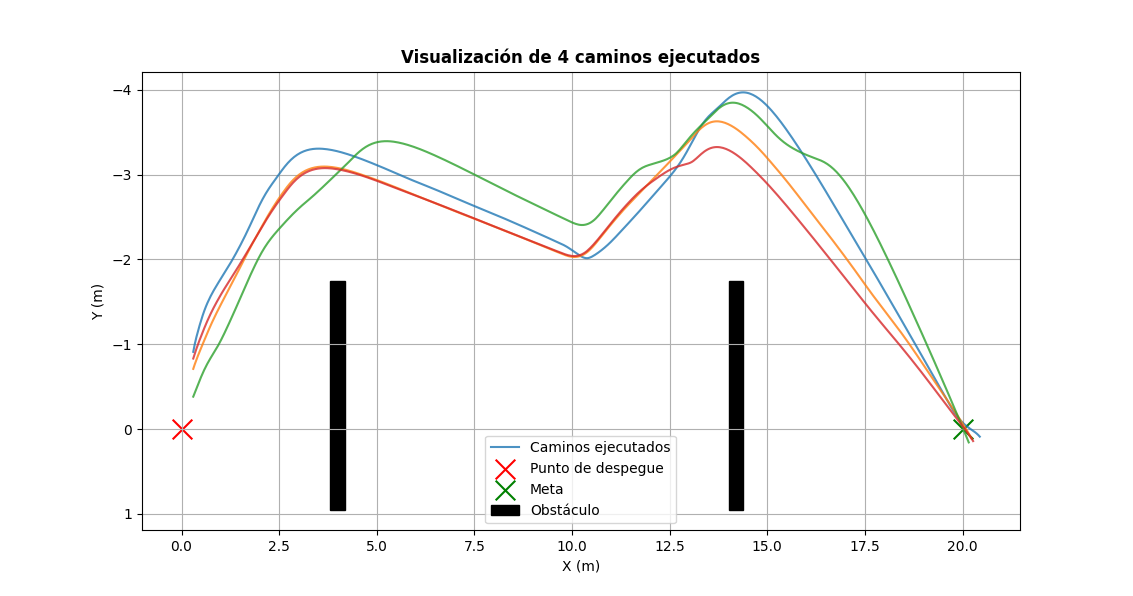
\includegraphics[scale=0.5]{partes/img/sim-double-panel-graph-4.png}
    \caption[Visualización simultánea de 4 caminos ejecutados dentro de la segunda configuración de obstáculos en entorno de simulación.]{Visualización simultánea de 4 caminos ejecutados dentro de la segunda configuración de obstáculos en entorno de simulación. De 10 vuelos ejecutados dentro de esta configuración, 10 resultaron sin colisión.}
    \label{fig:double-graph-4}
\end{figure}

En lo que respecta a la desviación máxima de los caminos ejecutados en esta configuración, la Figura \ref{fig:double-max-deviation} muestra un diagrama de caja de la desviación máxima de los caminos ejecutados. La desviación máxima promedio de los caminos ejecutados en esta configuración es cerca de 3.7 metros, con una desviación máxima de cerca de 4 metros y una desviación mínima de cerca de 3.3 metros. Estos resultados muestran como la maniobra para esquivar el segundo obstáculo incrementa la desviación máxima de los caminos ejecutados.

\begin{figure}[H]
    \centering
    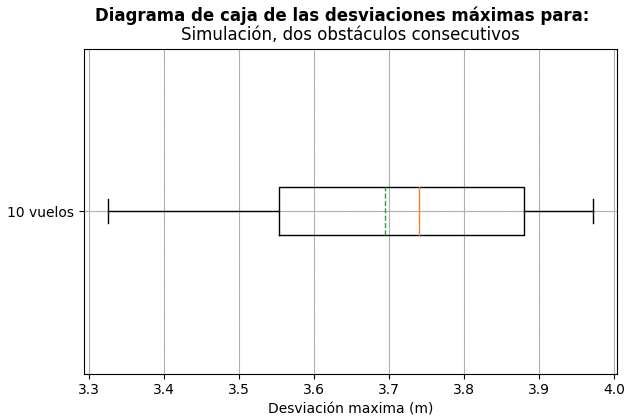
\includegraphics[scale=0.55]{partes/img/sim-double-panel-box.png}
    \caption[Diagrama de caja de la desviación máxima de los caminos ejecutados en la segunda configuración de obstáculos en entorno de simulación.]{Diagrama de caja de la desviación máxima de los caminos ejecutados en la segunda configuración de obstáculos en entorno de simulación.}
    \label{fig:double-max-deviation}
\end{figure}

Es interesante resaltar, que en los vuelos dentro de la segunda configuración, se confirma el funcionamiento del mecanismo que desactiva la inferencia cuando no hay obstáculos visibles. Para visualizar esto, se desarrolló una visualización 3D que permite visualizar la ejecución del algoritmo incluyendo la información sensorial de profundidad y las trayectorias generadas. En esta visualización se muestra:

\begin{itemize}
    \item La nube de puntos del entorno percibido por las cámaras estereoscópicas del QUAV, el color de los puntos indica la profundidad con respecto al sistema de cámaras, mientras más rojo más cerca y mientras más azul más lejos.
    \item El camino ejecutado por el QUAV, que se muestra como una curva de color blanco.
    \item La trayectoria más reciente generada por la política estudiante, que se muestra como una curva de color verde que comienza en la posición en donde se realizo la inferencia.
    \item El radio de colisión del QUAV, que se muestra como una circunferencia de color azul alrededor de la posición del QUAV. Si un obstáculo entra dentro de esta circunferencia se considera una colisión.
    \item La dirección del encabezamiento del QUAV, que se muestra como una línea roja que parte de la posición del QUAV.
    \item Las posiciones de despegue y de meta, que se muestran como un circulo rojo y verde respectivamente.
    \item El camino directo entre el punto de despegue y la meta.
    \item La orientación tridimensional del entorno, que se muestra como tres flechas; una azul que representa la dirección del eje \jim{z}, una verde que representa la dirección del eje \jim{y} y una roja que representa la dirección del eje \jim{x}. Es importante mencionar que debido a limitaciones del programa de visualización, la dirección del eje \jim{y} se encuentra invertida con respecto al resto de visualizaciones en este capítulo.
\end{itemize}

La Figura \ref{fig:depth-dual-panel-1}, la Figura \ref{fig:depth-dual-panel-2} y la Figura \ref{fig:depth-dual-panel-3} muestran capturas consecutivas de la visualización 3D de un vuelo dentro de la segunda configuración, desde una perspectiva de arriba hacia abajo. En estas figuras podemos observar como solo se generan trayectorias cuando hay un obstáculo cerca en el campo de visión del QUAV.

\begin{figure}[H]
    \centering
    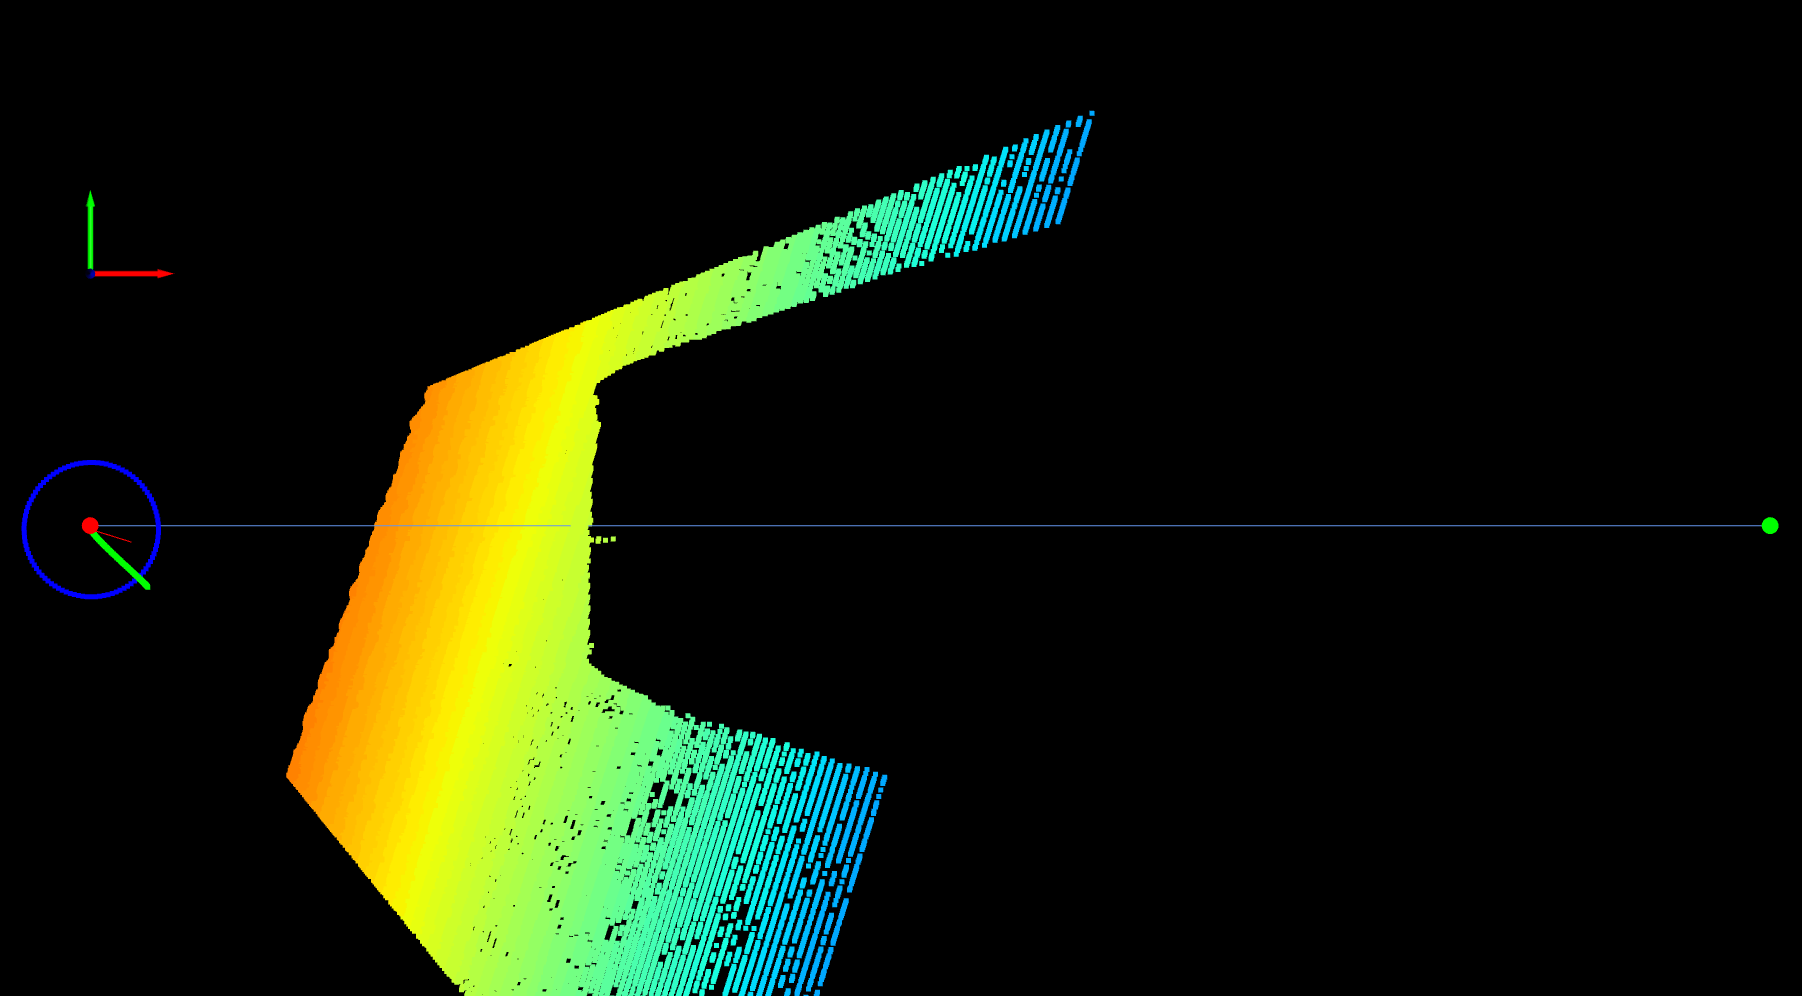
\includegraphics[scale=0.225]{partes/img/depth-dual-panel-1-first-obs.png}
    \caption[Visualización del funcionamiento del mecanismo que desactiva la inferencia cuando no hay obstáculos visibles. Inferencia activada, el primer obstáculo está en el campo de visión.]{Visualización del funcionamiento del mecanismo que desactiva la inferencia cuando no hay obstáculos visibles. Inferencia activada, el primer obstáculo está en el campo de visión.}
    \label{fig:depth-dual-panel-1}
\end{figure}

\begin{figure}[H]
    \centering
    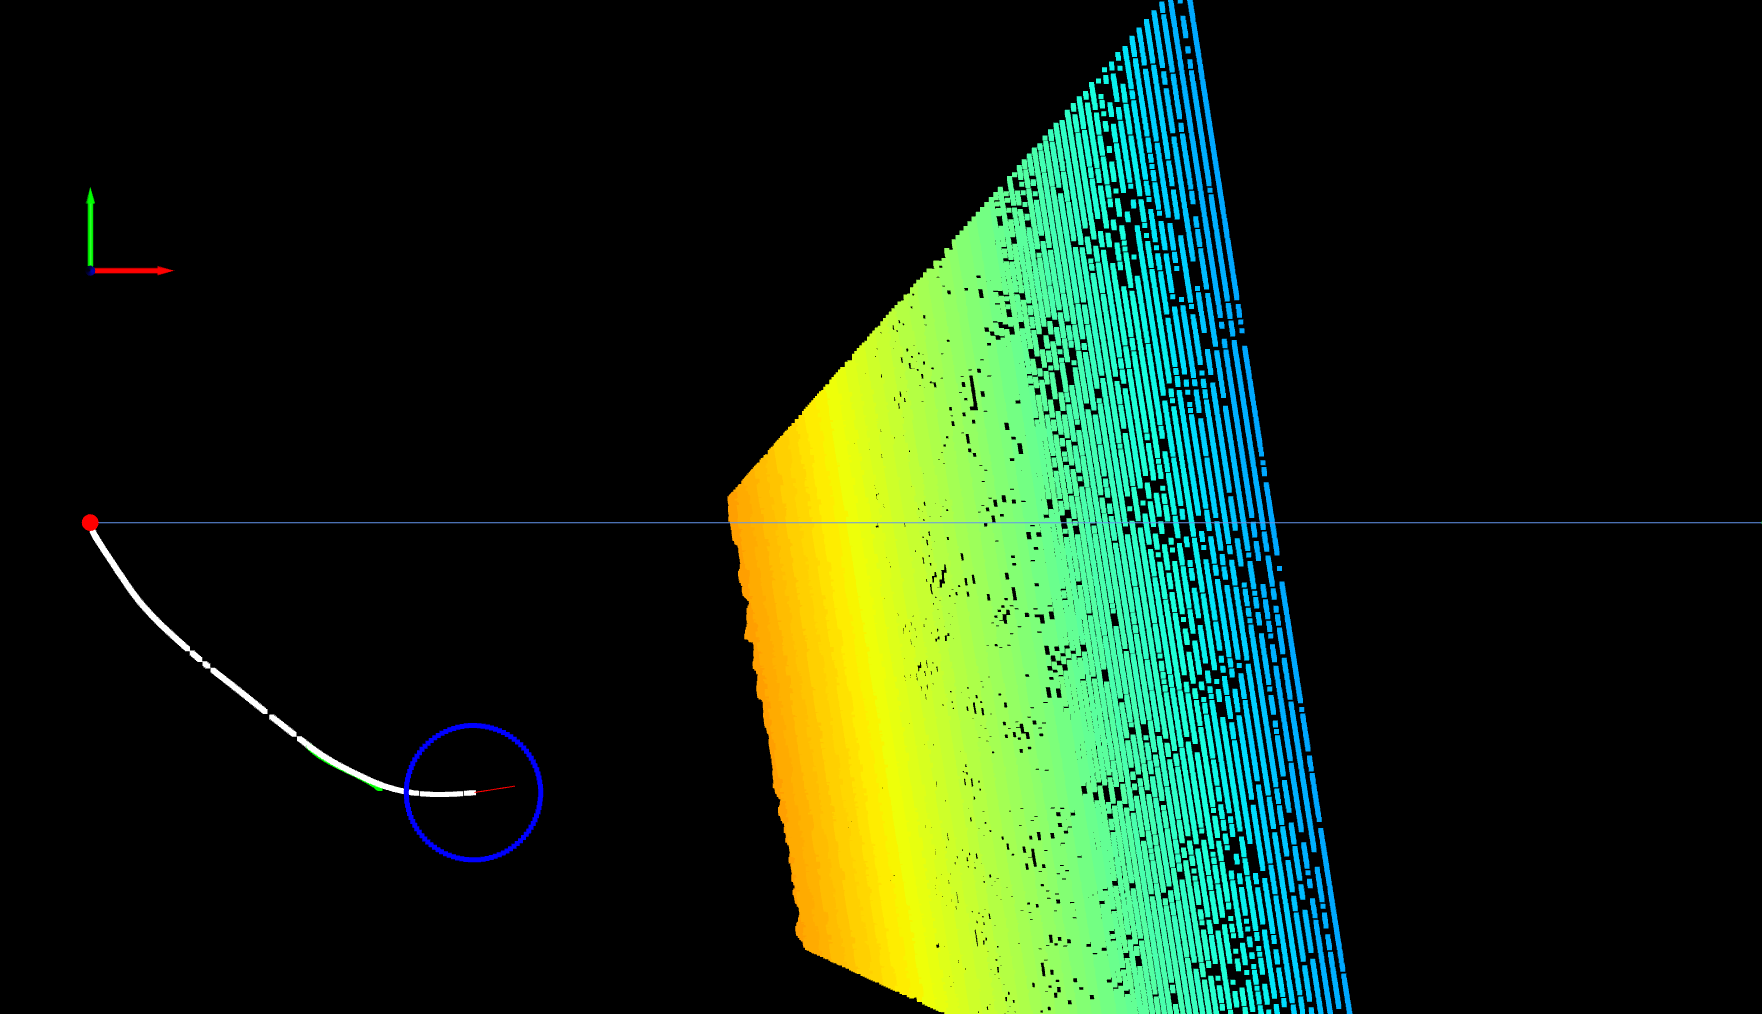
\includegraphics[scale=0.225]{partes/img/depth-dual-panel-2-no-obs.png}
    \caption[Visualización del funcionamiento del mecanismo que desactiva la inferencia cuando no hay obstáculos visibles. Inferencia desactivada, no hay obstáculo visible en campo de visión, navegando en dirección a la meta.]{Visualización del funcionamiento del mecanismo que desactiva la inferencia cuando no hay obstáculos visibles. Inferencia desactivada, no hay obstáculo visible en campo de visión, navegando en dirección a la meta.}
    \label{fig:depth-dual-panel-2}
\end{figure}

\begin{figure}[H]
    \centering
    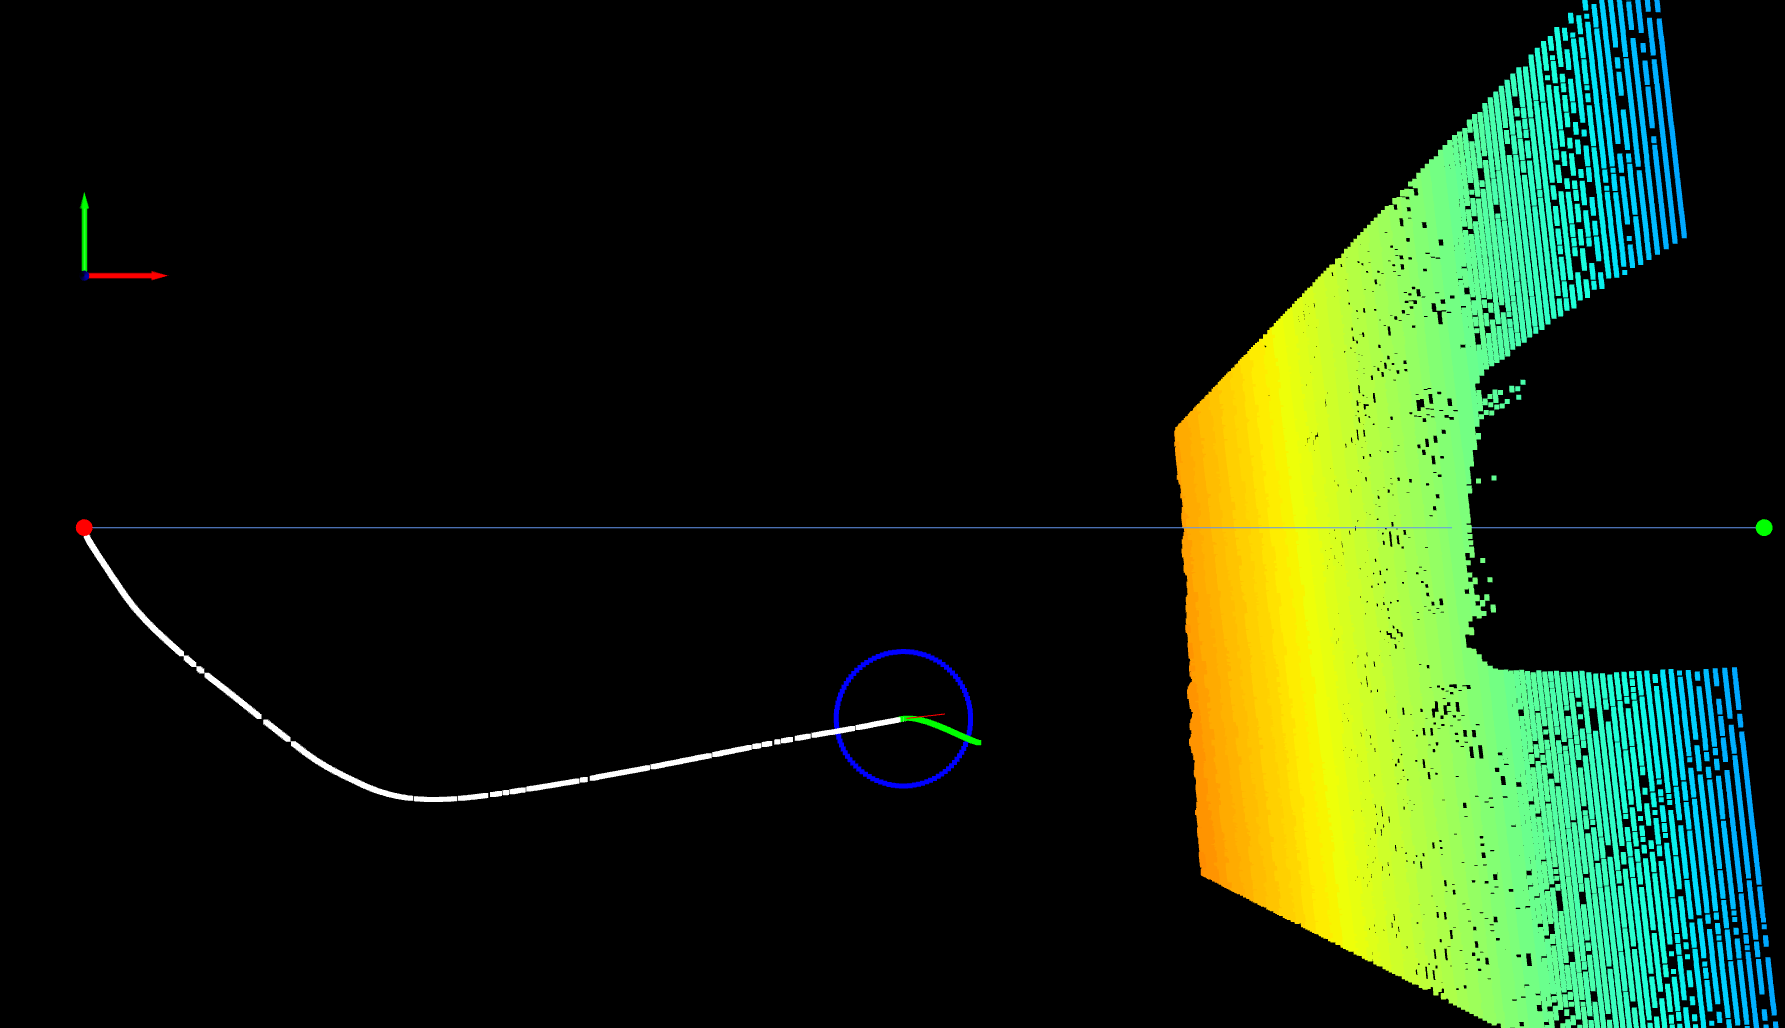
\includegraphics[scale=0.225]{partes/img/depth-dual-panel-3-second-obs.png}
    \caption[Visualización del funcionamiento del mecanismo que desactiva la inferencia cuando no hay obstáculos visibles. Inferencia activada, el segundo obstáculo está en el campo de visión.]{Visualización del funcionamiento del mecanismo que desactiva la inferencia cuando no hay obstáculos visibles. Inferencia activada, el segundo obstáculo está en el campo de visión.}
    \label{fig:depth-dual-panel-3}
\end{figure}

Durante todas las pruebas descritas anteriormente, se observó que la política de evasión de obstáculos tiene una preferencia certera a esquivar obstáculos en la dirección \jim{-y_B}, para evaluar este comportamiento el siguiente conjunto de pruebas utiliza una configuración que coloca un obstáculo adicional hacia esa dirección. La Figura \ref{fig:config-3-parallel} muestra la tercera configuración utilizada, que consiste de dos obstáculos simples paralelos entre si con una separación de 2 metros.

\begin{figure}[H]
    \centering
    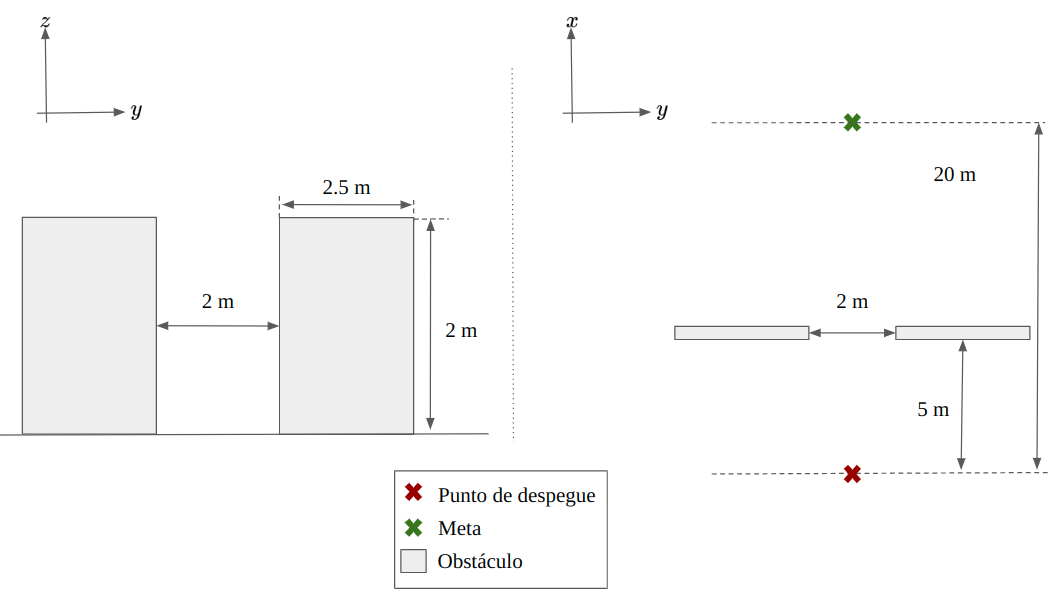
\includegraphics[scale=0.35]{partes/img/config-3-parallel.png}
    \caption[Tercera configuración de obstáculos dentro del entorno de AirSim.]{Tercera configuración de obstáculos dentro del entorno de AirSim. Dos obstáculos paralelos con una separación de 2 metros.}
    \label{fig:config-3-parallel}
\end{figure}

Incluso con la presencia de un obstáculo adicional en la dirección \jim{-y_B}, la política de evasión de obstáculos en todas las pruebas realizadas generó trayectorias dirigidas hacia \jim{-y_B}, lo cual produjo colisiones frecuentes, de 10 vuelos ejecutados, 2 fueron sin colisión. La Figura \ref{fig:depth-parallel-1}, la Figura \ref{fig:depth-parallel-2},  la Figura \ref{fig:depth-parallel-4} y la Figura \ref{fig:depth-parallel-5} muestran una secuencia consecutiva de capturas de la visualización 3D de un vuelo que resultó en colisión. Tal como se aprecia en las figuras, mientras ambos obstáculos son visibles en el campo de visión del QUAV, la trayectoria se dirige al espacio entre ambos obstáculos, con un comportamiento que parece guiar al QUAV a una ejecución sin colisiones; sin embargo, en el momento que solo un de los dos obstáculo es visible, en lugar de continuar dirigiéndose hacia el espacio entre ambos obstáculos, la política intenta corregir la trayectoria para esquivar por el flanco en dirección \jim{-y_B} relativo al obstáculo, lo cual produce una colisión. 

\begin{figure}[H]
    \centering
    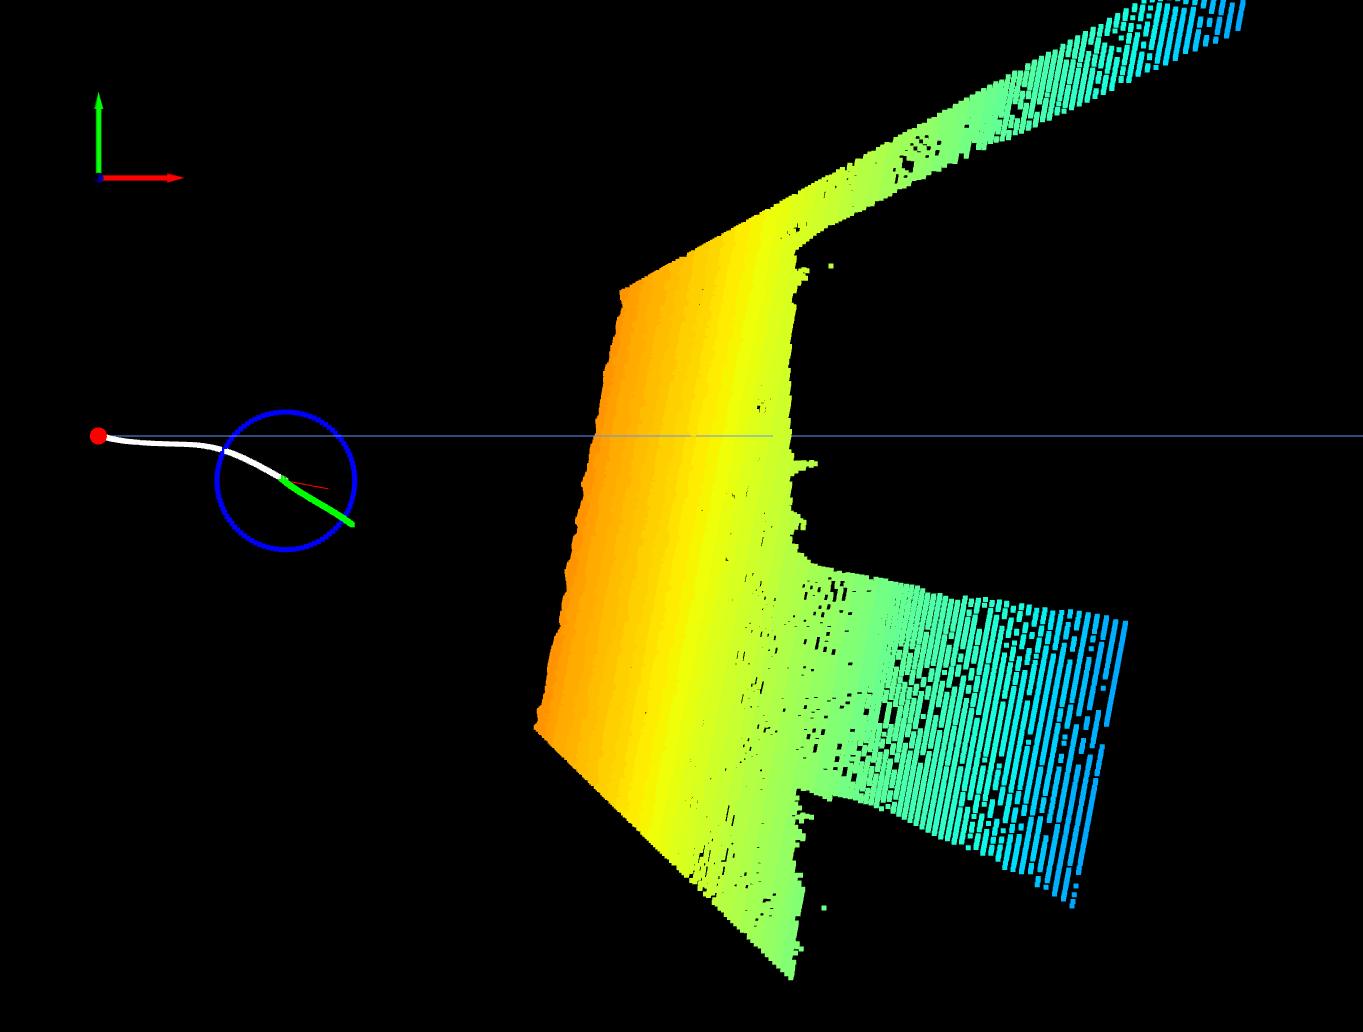
\includegraphics[scale=0.3]{partes/img/depth-parallel-1-topdown.png}
    \caption[Visualización 3D de un vuelo en la tercera configuración de obstáculos (1). Vista de arriba hacia abajo.]{Visualización 3D de un vuelo en la tercera configuración de obstáculos (1). Vista de arriba hacia abajo. Ambos obstáculos están dentro del campo de visión, las trayectorias generadas se dirigen hacia el espacio entre los obstáculos.}
    \label{fig:depth-parallel-1}
\end{figure}

\begin{figure}[H]
    \centering
    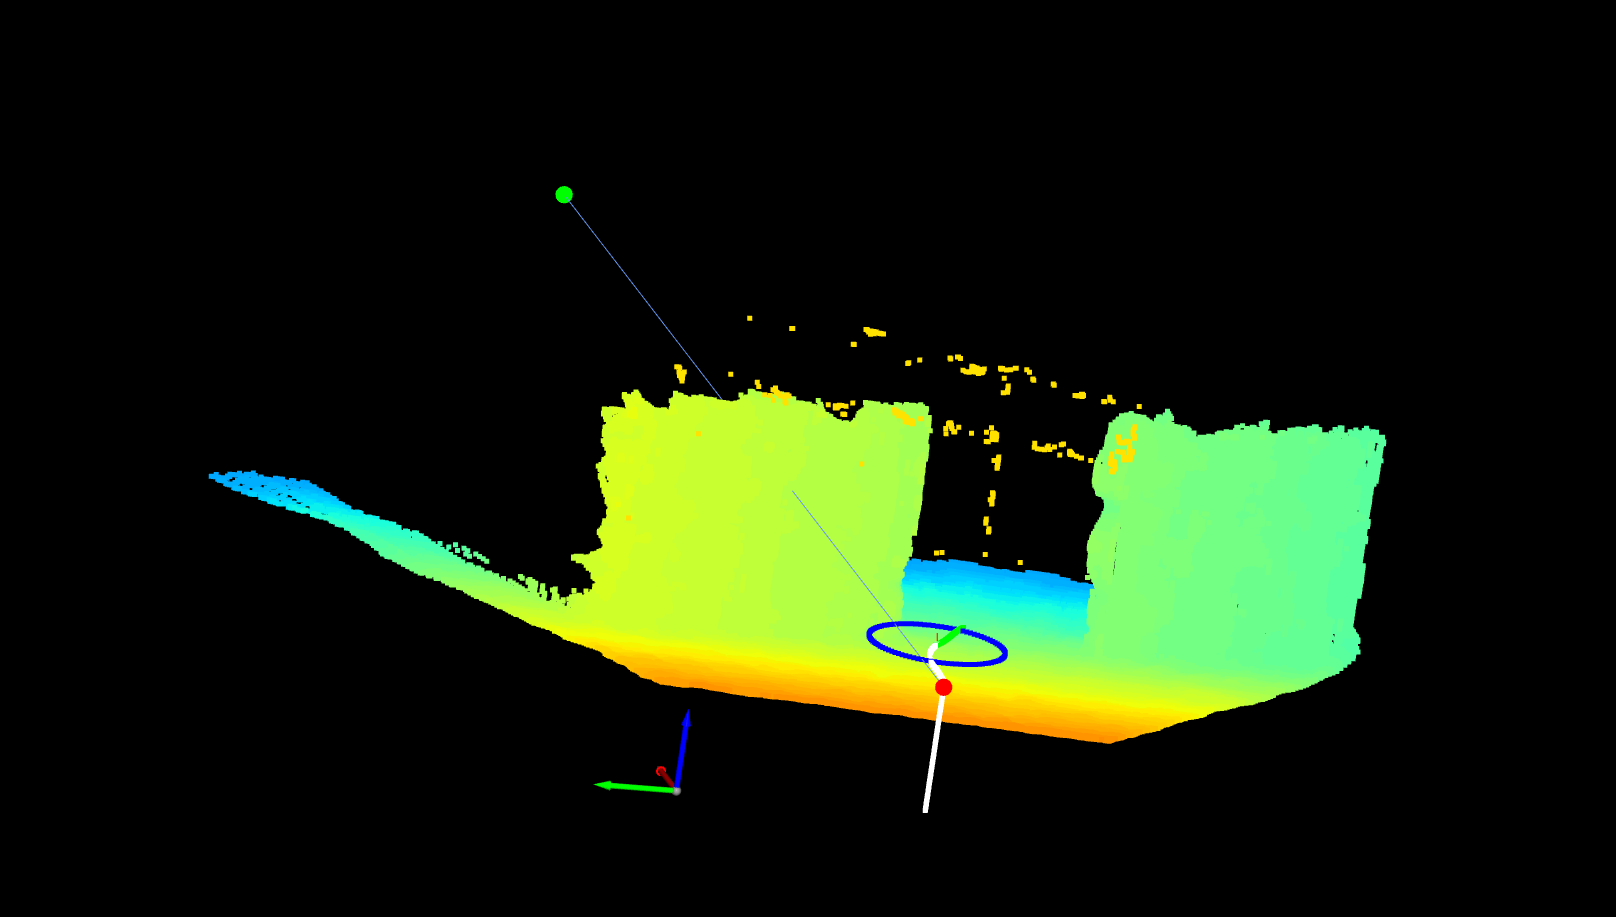
\includegraphics[scale=0.25]{partes/img/depth-parallel-2-front.png}
    \caption[Visualización 3D de un vuelo en la tercera configuración de obstáculos (2). Vista frontal.]{Visualización 3D de un vuelo en la tercera configuración de obstáculos (2). Vista frontal. Ambos obstáculos están dentro del campo de visión, las trayectorias generadas se dirigen hacia el espacio entre los obstáculos.}
    \label{fig:depth-parallel-2}
\end{figure}

\begin{figure}[H]
    \centering
    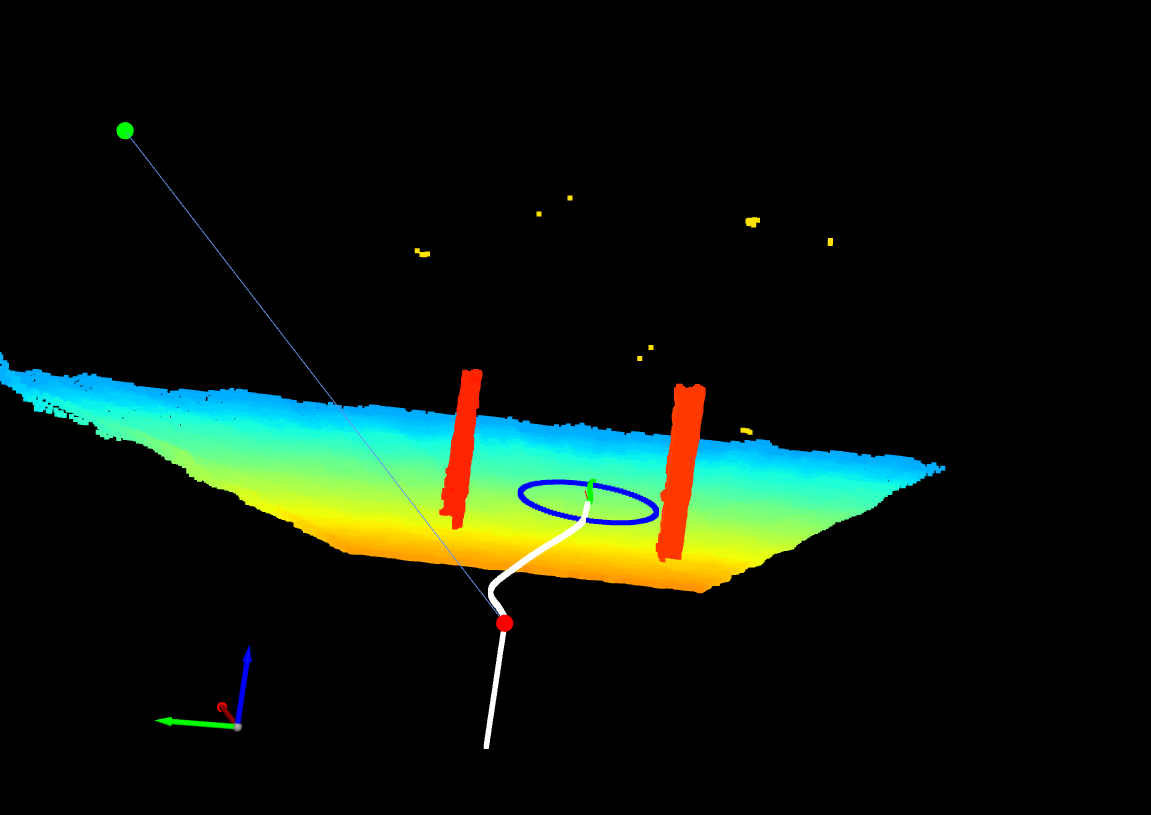
\includegraphics[scale=0.32]{partes/img/depth-parallel-4-front-red.png}
    \caption[Visualización 3D de un vuelo en la tercera configuración de obstáculos (3). Vista frontal. Navegando entre el espacio entre los obstáculos.]{Visualización 3D de un vuelo en la tercera configuración de obstáculos (3). Vista frontal. Navegando entre el espacio entre los obstáculos. Ambos obstáculos están dentro del campo de visión, las trayectorias generadas se dirigen hacia el espacio entre los obstáculos.}
    \label{fig:depth-parallel-4}
\end{figure}

\begin{figure}[H]
    \centering
    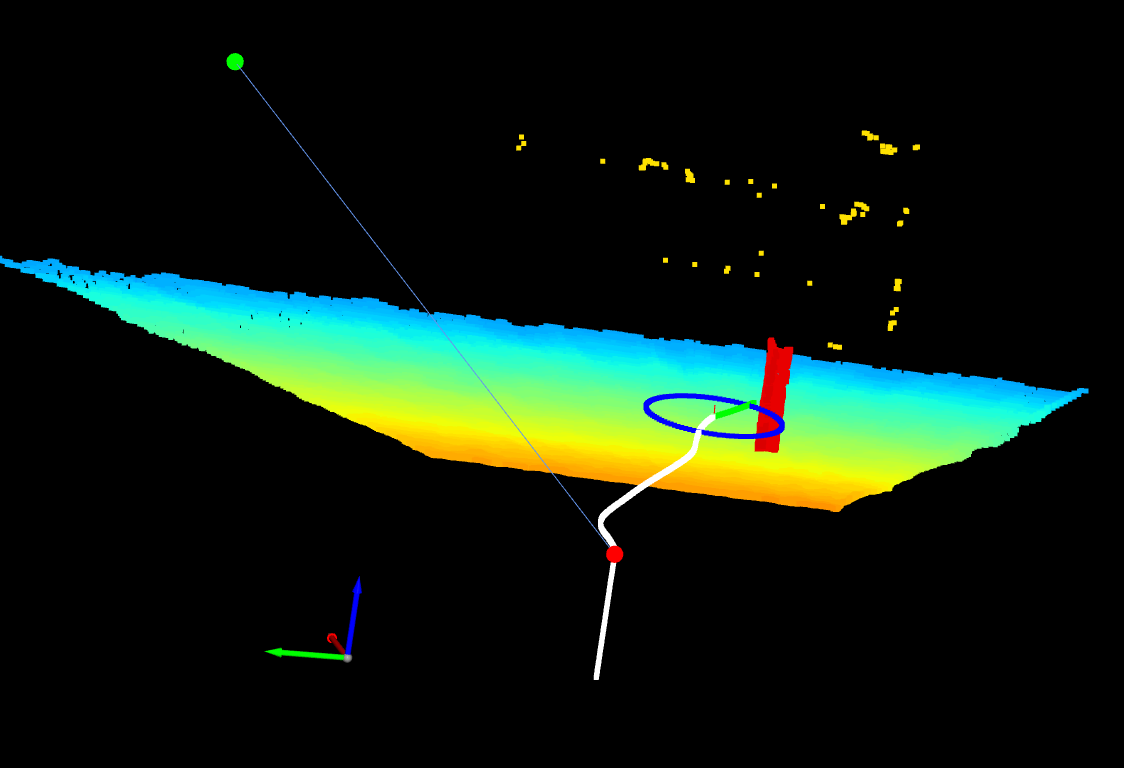
\includegraphics[scale=0.32]{partes/img/depth-parallel-5-front-collision.png}
    \caption[Visualización 3D de un vuelo en la tercera configuración de obstáculos (4). Vista frontal. Colisión.]{Visualización 3D de un vuelo en la tercera configuración de obstáculos (4). Vista frontal. En el momento que uno de los dos obstáculos desaparece del campo de visión, en lugar de continuar dirigiéndose hacia el espacio entre ambos obstáculos, la política intenta corregir la trayectoria para esquivar por el flanco en dirección \jim{-y_B} relativo al obstáculo, lo cual produce una colisión. }
    \label{fig:depth-parallel-5}
\end{figure}


Para evaluar esta preferencia fuerte a esquivar por el flanco en la dirección \jim{-y_B} con respecto al obstáculo, la siguiente configuración a evaluar es de tal forma que no existe una forma de esquivar por el flanco en la dirección \jim{-y_B} sin regresar hacia atrás, la Figura \ref{fig:config-4-wall} muestra un diagrama de la configuración en cuestión.

\begin{figure}[H]
    \centering
    \includegraphics[scale=0.31]{partes/img/config-4-left-wall.png}
    \caption[Cuarta configuración de obstáculos dentro del entorno de AirSim.]{Cuarta configuración de obstáculos dentro del entorno de AirSim. Obstáculo simple con pared del lado izquierdo.}
    \label{fig:config-4-wall}
\end{figure}

Todos los vuelos realizados en esta configuración terminaron en una colisión. La Figura \ref{depth-wall-1}, la Figura \ref{depth-wall-2}, la Figura \ref{depth-wall-3}, la Figura \ref{depth-wall-4} y la Figura \ref{depth-wall-5} muestran una secuencia consecutiva de capturas de la visualización 3D de un vuelo en esta configuración que resultó en colisión. En las figuras se observa como la política de evasión de obstáculos intenta generar trayectorias que se dirigen hacia la región en la dirección \jim{-y_B} en donde no hay información de profundidad, probablemente esperando encontrar el borde del obstáculo en esa dirección, pero como en esta configuración de obstáculos ese borde se encuentra hacia atrás, se produce una colisión.

\begin{figure}[H]
    \centering
    \includegraphics[scale=0.23]{partes/img/depth-wall-1-front.png}
    \caption[Visualización 3D de un vuelo en la cuarta configuración de obstáculos (1). Vista frontal.]{Visualización 3D de un vuelo en la cuarta configuración de obstáculos (1). Vista frontal.}
    \label{depth-wall-1}
\end{figure}

\begin{figure}[H]
    \centering
    \includegraphics[scale=0.25]{partes/img/depth-wall-2-top.png}
    \caption[Visualización 3D de un vuelo en la cuarta configuración de obstáculos (2). Vista de arriba hacia abajo. Búsqueda del borde del obstáculo.]{Visualización 3D de un vuelo en la cuarta configuración de obstáculos (2). Vista de arriba hacia abajo. Las trayectorias se dirigen hacia la región en dirección \jim{-y_B} sin información de profundidad, probablemente buscando el borde del obstáculo.}
    \label{depth-wall-2}
\end{figure}

\begin{figure}[H]
    \centering
    \includegraphics[scale=0.25]{partes/img/depth-wall-3-try-arround.png}
    \caption[Visualización 3D de un vuelo en la cuarta configuración de obstáculos (3). Vista de arriba hacia abajo. Búsqueda del borde del obstáculo.]{Visualización 3D de un vuelo en la cuarta configuración de obstáculos (3). Vista de arriba hacia abajo. Las trayectorias continúan dirigiéndose hacia la región en dirección \jim{-y_B} sin información de profundidad, probablemente buscando el borde del obstáculo.}
    \label{depth-wall-3}
\end{figure}

\begin{figure}[H]
    \centering
    \includegraphics[scale=0.25]{partes/img/depth-wall-4-still-go-arround.png}
    \caption[Visualización 3D de un vuelo en la cuarta configuración de obstáculos (4). Vista de arriba hacia abajo. Búsqueda del borde del obstáculo.]{Visualización 3D de un vuelo en la cuarta configuración de obstáculos (4). Vista de arriba hacia abajo. Las trayectorias continúan dirigiéndose hacia la región en dirección \jim{-y_B} sin información de profundidad, probablemente buscando el borde del obstáculo.}
    \label{depth-wall-4}
\end{figure}

\begin{figure}[H]
    \centering
    \includegraphics[scale=0.25]{partes/img/depth-wall-5-crash.png}
    \caption[Visualización 3D de un vuelo en la cuarta configuración de obstáculos (5). Vista de arriba hacia abajo. Colisión.]{Visualización 3D de un vuelo en la cuarta configuración de obstáculos. Vista de arriba hacia abajo. Al no conseguir el borde del obstáculo a tiempo, se produce una colisión.}
    \label{depth-wall-5}
\end{figure}

De estos resultados se confirma que los efectos consecuencia de las dificultades encontradas durante el refinamiento fino de la política estudiante son la preferencia certera a esquivar obstáculos hacia el flanco izquierdo (en dirección \jim{-y_B}), y que estos efectos producen colisiones en configuraciones de obstáculos donde no es posible esquivar hacia ese flanco.

En la Tabla \ref{table:sim-results} se muestra un resumen de los resultados obtenidos en los vuelos en simulación. En esta tabla se muestra que la política es estable para las configuraciones de obstáculos donde es trivial esquivar por el flanco izquierdo. De igual forma, se muestra que la política es inestable y propensa a producir colisiones para las configuraciones de obstáculos donde es no trivial esquivar por el flanco izquierdo.

\begin{table}[h]
\centering
\begin{tabular}{||c || c | c | c | c | c | c||} 
 \hline
 \textbf{Configuración} & \jim{N} & \jim{N_{e}} & \textbf{P} & \jim{\bar{D}} & \jim{\max(D)} & \jim{\min(D)} \rule{0pt}{2.6ex} \\ [0.4ex] 
 \hline\hline
 Obstáculo simple              & 10 & 10 & \textbf{100\%} & 3.1 & 3.4 & 2.7 \\ 
 \hline
 Dos obstáculos consecutivos   & 10 & 10 & \textbf{100\%} & 3.7 & 4 & 3.3 \\
 \hline
 Dos obstáculos paralelos      & 10 & 2  & \textbf{20 \%} & N/A & N/A & N/A \\
 \hline
 Obstáculo con pared izquierda & 10 & 0  & \textbf{0  \%} & N/A & N/A & N/A \\
 \hline
\end{tabular}
\caption[Resumen de los resultados obtenidos en los vuelos en simulación.]{Resumen de los resultados obtenidos en los vuelos en simulación. \jim{N} y \jim{N_{e}} son el número de vuelos totales y sin colisión respectivamente. \textbf{P} es el porcentaje de vuelos sin colisión. \jim{\bar{D}}, \jim{\max(D)} y \jim{\min(D)} son la desviación máxima promedio, máxima y mínima respectivamente (en metros).}
\label{table:sim-results}
\end{table}

\subsection{Vuelos sobre la plataforma física}

\label{sec:results-SOTEN}

En esta sección se describen las configuraciones y resultados de los vuelos realizados sobre la plataforma física de implementación (QUAV SOTEN\footnote[1]{En la Figura \ref{fig:SOTEN} se muestra al QUAV SOTEN.}) en un entorno de la vida real. Esto vuelos fueron ejecutados en un campo de vuelo para drones ubicado en la prefectura de Chiba, Japón; las condiciones climáticas del día fueron: soleado con un ligero viento en dirección hacia el oeste. Durante los vuelos, un piloto experto estuvo preparado para controlar manualmente el QUAV en caso de que una colisión fuera inminente. En esta sección se utiliza el termino ``colision'' para referirse al evento de interrumpir el vuelo autónomo para evitar una colisión inminente. Al igual que durante los vuelos en simulación, la ejecución de la evasión de obstáculos está limitada al plano \jim{xy} del marco de referencia del cuerpo del QUAV.

La primera configuración de obstáculos utilizada fue una configuración simple con un solo obstáculo en la línea directa de visión del QUAV, la Figura \ref{real-1-single-0-setup} muestra una fotografía ilustrada que describe la configuración.

\begin{figure}[H]
    \centering
    \includegraphics[scale=0.22]{partes/img/real-1-single-0-setup.png}
    \caption[Configuración de obstáculos en entorno real: Obstáculo simple]{Configuración de obstáculos en entorno real: Obstáculo simple.}
    \label{real-1-single-0-setup}
\end{figure}

Se realizaron 11 vuelos en esta configuración, y los resultados fueron análogos a los obtenidos en simulación, en concreto, de 11 vuelos ejecutados, 10 resultaron sin colisión y uno fue abortado por el piloto debido a la influencia de una fuerte ráfaga de viento. Los caminos resultantes de los vuelos también fueron análogos a los obtenidos en simulación, sin embargo, debido a variaciones en el viento y en las condiciones de iluminación, algunas ejecuciones se desviaron considerablemente del camino directo. La Figura \ref{real-1-single-graph} muestra una visualización de arriba hacia abajo de 10 de los caminos ejecutados en esta configuración, incluyendo el vuelo que fue abortado por el piloto. Se puede observar que la desviación máxima de los caminos ejecutados con respecto al camino directo entre el punto de despegue y la meta varía bastante entre vuelos (probablemente debido a las variaciones en el viento), la Figura \ref{real-1-single-box} muestra un diagrama de caja de la desviación máxima de los caminos ejecutados en esta configuración. La desviación máxima promedio de los caminos ejecutados en esta configuración es cerca de 3.2 metros, con una desviación máxima de cerca de 4.5 metros y una desviación mínima de cerca de 2 metros.

\begin{figure}[H]
    \centering
    \includegraphics[scale=0.55]{partes/img/real-1-single-graph-all.png}
    \caption[Visualización de 10 caminos ejecutados en la primera configuración de obstáculos en entorno real.]{Visualización de 10 caminos ejecutados en la primera configuración de obstáculos en entorno real. Incluyendo el vuelo que fue abortado por el piloto.}
    \label{real-1-single-graph}
\end{figure}

\begin{figure}[H]
    \centering
    \includegraphics[scale=0.7]{partes/img/real-1-single-box.png}
    \caption[Diagrama de caja de la desviación máxima de los caminos ejecutados en la primera configuración de obstáculos en entorno real.]{Diagrama de caja de la desviación máxima de los caminos ejecutados en la primera configuración de obstáculos en entorno real.}
    \label{real-1-single-box}
\end{figure}

En todos los vuelos ejecutados en esta configuración, el algoritmo esquivó el obstáculo por el flanco izquierdo y continuo en dirección a la meta. La Figura \ref{real-1-single-3-frames-1}, la Figura \ref{real-1-single-3-frames-2} y la Figura \ref{real-1-single-3-frames-3} muestran capturas de una grabación de uno de los vuelos sobre esta configuración. La Figura \ref{real-1-single-4-frames-1}, la Figura \ref{real-1-single-4-frames-2} y la Figura \ref{real-1-single-4-frames-3} también muestran capturas de una grabación de uno de los vuelos sobre esta configuración pero en una perspectiva diferente. En estas figuras se aprecia claramente el comportamiento del algoritmo, en particular: comenzar el vuelo, esquivar el obstáculo por el flanco izquierdo, continuar avanzando hasta que se termine la trayectoria actual y finalmente, como no se observan obstáculos, navegar en dirección a la meta.

\begin{figure}[H]
    \centering
    \includegraphics[scale=0.25]{partes/img/real-1-single-3-frames-1.png}
    \caption[Capturas de una grabación de uno de los vuelos en entorno real con un obstáculo simple (1).]{Capturas de una grabación de uno de los vuelos en entorno real con un obstáculo simple (1). \textbf{(a)} Comienza el vuelo. \textbf{(b)} Se comienza a esquivar el obstáculo.}
    \label{real-1-single-3-frames-1}
\end{figure}

\begin{figure}[H]
    \centering
    \includegraphics[scale=0.255]{partes/img/real-1-single-3-frames-2.png}
    \caption[Capturas de una grabación de uno de los vuelos en entorno real con un obstáculo simple (2).]{Capturas de una grabación de uno de los vuelos en entorno real con un obstáculo simple (2). En \textbf{(c)} y \textbf{(d)}, se esquiva el obstáculo por el flanco izquierdo.}
    \label{real-1-single-3-frames-2}
\end{figure}

\begin{figure}[H]
    \centering
    \includegraphics[scale=0.245]{partes/img/real-1-single-3-frames-3.png}
    \caption[Capturas de una grabación de uno de los vuelos en entorno real con un obstáculo simple (3).]{Capturas de una grabación de uno de los vuelos en entorno real con un obstáculo simple (3). En \textbf{(e)} y \textbf{(f)}, como no se observan obstáculos, se navega en dirección a la meta.}
    \label{real-1-single-3-frames-3}
\end{figure}

\begin{figure}[H]
    \centering
    \includegraphics[scale=0.24]{partes/img/real-1-single-4-frames-1.png}
    \caption[Capturas de una grabación de uno de los vuelos en entorno real con un obstáculo simple. Vista frontal (1).]{Capturas de una grabación de uno de los vuelos en entorno real con un obstáculo simple. Vista frontal (1). \textbf{(a)} Antes del despegue. \textbf{(b)} Comienza el vuelo.}
    \label{real-1-single-4-frames-1}
\end{figure}

\begin{figure}[H]
    \centering
    \includegraphics[scale=0.24]{partes/img/real-1-single-4-frames-2.png}
    \caption[Capturas de una grabación de uno de los vuelos en entorno real con un obstáculo simple. Vista frontal (2).]{Capturas de una grabación de uno de los vuelos en entorno real con un obstáculo simple. Vista frontal (2). En \textbf{(c)} y \textbf{(d)}, se esquiva el obstáculo por el flanco izquierdo.}
    \label{real-1-single-4-frames-2}
\end{figure}

\begin{figure}[H]
    \centering
    \includegraphics[scale=0.24]{partes/img/real-1-single-4-frames-3.png}
    \caption[Capturas de una grabación de uno de los vuelos en entorno real con un obstáculo simple. Vista frontal (3).]{Capturas de una grabación de uno de los vuelos en entorno real con un obstáculo simple. Vista frontal (3). En \textbf{(e)} y \textbf{(f)}, como no se observan obstáculos, se navega en dirección a la meta.}
    \label{real-1-single-4-frames-3}
\end{figure}

La segunda configuración de obstáculos utilizada fue una configuración con dos obstáculos paralelos con una separación entre si, esta separación fue distinta para cada vuelo. A diferencia de la configuración anterior, en esta configuración solo se hicieron 3 vuelos. El objetivo de estos vuelos era observar el comportamiento del algoritmo en este escenario, en particular, confirmar la presencia de la tendencia certera de esquivar obstáculos por el flanco izquierdo que se observó durante vuelos análogos en entornos de simulación; así como también observar si esta tendencia produce colisiones inminentes.

En el primer vuelo en esta configuración se utilizó una separación de 3 metros, la Figura \ref{real-2-parallelA-0-config} muestra una fotografía que ilustra la configuración utilizada. Este vuelo fue abortado por colisión inminente, la Figura \ref{real-2-parallelA-1-frames} muestra capturas de la grabación de este vuelo en donde se observa el comportamiento del algoritmo. Primero (Figura \ref{real-2-parallelA-1-frames}(a)), la ejecución comienza; segundo (Figura \ref{real-2-parallelA-1-frames}(b)), el QUAV se dirige hacia el espacio entre ambos obstáculos en lugar de esquivar los obstáculos por el flanco derecho; y tercero (Figura \ref{real-2-parallelA-1-frames}(c)), cuando el obstáculo derecho sale del campo de visión, el algoritmo intenta esquivar el obstáculo que aun es visible por el flanco izquierdo, lo cual produce una colisión inminente, haciendo que el piloto tenga que abortar el vuelo. Estos resultados coinciden con el comportamiento observado en simulación \footnote[1]{Vea la Figura \ref{fig:depth-parallel-5}}, y confirman la presencia de la tendencia certera a esquivar obstáculos por el flanco izquierdo.

\begin{figure}[H]
    \centering
    \includegraphics[scale=0.22]{partes/img/real-2-parallelA-0-config.png}
    \caption[Configuración de obstáculos en entorno real: Obstáculos paralelos a 3 metros de separación.]{Configuración de obstáculos en entorno real: Obstáculos paralelos a 3 metros de separación.}
    \label{real-2-parallelA-0-config}
\end{figure}

\begin{figure}[H]
    \centering
    \includegraphics[scale=0.25]{partes/img/real-2-parallelA-1-frames.png}
    \caption[Capturas de la grabación del vuelo en entorno real con obstáculos paralelos a 3 metros de separación.]{Capturas de la grabación del vuelo en entorno real con obstáculos paralelos a 3 metros de separación. \textbf{(a)} La ejecución comienza. \textbf{(b)} El QUAV se dirige hacia el espacio entre ambos obstáculos en lugar de esquivar los obstáculos por el flanco derecho. \textbf{(c)} Cuando el obstáculo derecho sale del campo de visión, el algoritmo intenta esquivar el obstáculo que aun es visible por el flanco izquierdo, lo cual produce una colisión inminente.}
    \label{real-2-parallelA-1-frames}
\end{figure}

El segundo vuelo en la configuración de obstáculos paralelos utilizó una separación de 4 metros, la Figura \ref{real-3-parallelB-0-config} muestra una fotografía que ilustra la configuración utilizada. Este vuelo resultó exitoso, la Figura \ref{real-3-parallelB-1-frames} muestra capturas de la grabación de este vuelo en donde se observa el comportamiento del algoritmo. Primero (Figura \ref{real-3-parallelB-1-frames}(a)), la ejecución comienza y el QUAV navega hacia el espacio entre los dos obstáculos; segundo (Figura \ref{real-3-parallelB-1-frames}(b)), esta vez, el obstáculo izquierdo sale del campo de visión, y el QUAV continúa hacia el espacio entre los dos obstáculos; y tercero (Figura \ref{real-3-parallelB-1-frames}(c)), se superan los obstáculos y se navega en dirección a la meta. De este vuelo confirmamos que si la configuración de obstáculos paralelos es tal que el primer obstáculo que desaparece el campo de visión es el obstáculo izquierdo, entonces es posible que el algoritmo sea capaz de completar el vuelo sin producir colisiones. La Figura \ref{real-3-parallelB-2-graph} muestra una visualización de arriba hacia abajo del camino ejecutado por el QUAV en este vuelo.

\begin{figure}[H]
    \centering
    \includegraphics[scale=0.27]{partes/img/real-3-parallelB-0-config.png}
    \caption[Configuración de obstáculos en entorno real: Obstáculos paralelos a 4 metros de separación.]{Configuración de obstáculos en entorno real: Obstáculos paralelos a 4 metros de separación.}
    \label{real-3-parallelB-0-config}
\end{figure}

\begin{figure}[H]
    \centering
    \includegraphics[scale=0.25]{partes/img/real-3-parallelB-1-frames.png}
    \caption[Capturas de la grabación del vuelo en entorno real con obstáculos paralelos a 4 metros de separación.]{Capturas de la grabación del vuelo en entorno real con obstáculos paralelos a 4 metros de separación. \textbf{(a)} La ejecución comienza y el QUAV navega hacia el espacio entre los dos obstáculos. \textbf{(b)} El obstáculo izquierdo sale del campo de visión, y el QUAV continúa hacia el espacio entre los dos obstáculos. \textbf{(c)}  Se superan los obstáculos y se navega en dirección a la meta.}
    \label{real-3-parallelB-1-frames}
\end{figure}

\begin{figure}[H]
    \centering
    \includegraphics[scale=0.5]{partes/img/real-3-parallelB-2-graph.png}
    \caption[Visualización del camino ejecutado por el QUAV para la configuración de obstáculos paralelos a 4 metros de separación en entorno real.]{Visualización del camino ejecutado por el QUAV para la configuración de obstáculos paralelos a 4 metros de separación en entorno real.}
    \label{real-3-parallelB-2-graph}
\end{figure}

El tercer y último vuelo en la configuración de obstáculos paralelos utilizó una separación de un metro, la Figura \ref{real-4-parallelC-0-config} muestra una fotografía que ilustra la configuración utilizada. Este vuelo resultó exitoso y la razón por la cual fue exitoso provee información adicional sobre la capacidad de evasión de obstáculos del algoritmo. La Figura \ref{real-4-parallelC-1-frames} muestra capturas de la grabación de este vuelo en donde se observa el comportamiento del algoritmo. Primero (Figura \ref{real-4-parallelC-1-frames}(a)), la ejecución comienza y el QUAV navega hacia el espacio entre los dos obstáculos; segundo (Figura \ref{real-4-parallelC-1-frames}(b)), en el momento que el obstáculo izquierdo se vuelve el obstáculo mas grande en el campo de visión, el algoritmo intenta fuertemente corregir la trayectoria para esquivar el conjunto de obstáculos por el flanco izquierdo del obstáculo izquierdo, esto ocurre tempranamente en el vuelo pues la separación entre los obstáculos es relativamente pequeña; y tercero (Figura \ref{real-4-parallelC-1-frames}(c)), como la decisión de de corregir la trayectoria hacia la izquierda ocurre de forma temprana, el algoritmo tiene tiempo de completar la trayectoria sin producir colisiones, resultando en una ejecución exitosa. La Figura \ref{real-4-parallelC-2-graph} muestra una visualización de arriba hacia abajo del camino ejecutado por el QUAV en esta configuración, en donde se evidencia el momento en el que el algoritmo intenta corregir fuertemente; adicionalmente, para respladar la magnitud de la corrección en la Figura \ref{real-4-parallelC-3-yaw} se muestra el grafico del encabezamiento del QUAV en función del tiempo, en donde se observan oscilaciones de relativamente alta magnitud. El resultado de este vuelo expone que si existe el espacio y el tiempo para esquivar un conjunto de obstáculos por el flanco mas hacia la izquierda, es posible que la política de evasión de obstáculos sea capaz de completar el vuelo exitosamente.

\begin{figure}[H]
    \centering
    \includegraphics[scale=0.25]{partes/img/real-4-parallelC-0-config.png}
    \caption[Configuración de obstáculos en entorno real: Obstáculos paralelos a 1 metro de separación.]{Configuración de obstáculos en entorno real: Obstáculos paralelos a 1 metro de separación.}
    \label{real-4-parallelC-0-config}
\end{figure}

\begin{figure}[H]
    \centering
    \includegraphics[scale=0.24]{partes/img/real-4-parallelC-1-frames.png}
    \caption[Capturas de la grabación del vuelo en entorno real con obstáculos paralelos a 1 metro de separación.]{Capturas de la grabación del vuelo en entorno real con obstáculos paralelos a 1 metro de separación. \textbf{(a)} La ejecución comienza y el QUAV navega hacia el espacio entre los dos obstáculos. \textbf{(b)} El obstáculo izquierdo se vuelve el obstáculo mas grande en el campo de visión y el algoritmo intenta fuertemente corregir la trayectoria para esquivar el conjunto de obstáculos por el flanco izquierdo del obstáculo izquierdo. \textbf{(c)} Como la decisión de de corregir la trayectoria hacia la izquierda ocurre de forma temprana, el algoritmo tiene tiempo de completar la trayectoria sin producir colisiones, resultando en una ejecución exitosa. }
    \label{real-4-parallelC-1-frames}
\end{figure}

\begin{figure}[H]
    \centering
    \includegraphics[scale=0.5]{partes/img/real-4-parallelC-2-graph.png}
    \caption[Visualización del camino ejecutado por el QUAV para la configuración de obstáculos paralelos a 1 metro de separación en entorno real.]{Visualización del camino ejecutado por el QUAV para la configuración de obstáculos paralelos a 1 metro de separación en entorno real. Se puede observar el momento en el que el algoritmo intenta corregir fuertemente la trayectoria hacia la izquierda.}
    \label{real-4-parallelC-2-graph}
\end{figure}

\begin{figure}[H]
    \centering
    \includegraphics[scale=0.8]{partes/img/real-4-parallelC-3-yaw.png}
    \caption[Grafico del encabezamiento del QUAV en función del tiempo para la configuración de obstáculos paralelos a 1 metro de separación en entorno real.]{Grafico del encabezamiento del QUAV en función del tiempo para la configuración de obstáculos paralelos a 1 metro de separación en entorno real. Se observan oscilaciones de relativamente alta magnitud que corresponden al momento en el que el algoritmo intenta corregir fuertemente la trayectoria hacia la izquierda.}
    \label{real-4-parallelC-3-yaw}
\end{figure}

Los vuelos realizados permiten evaluar la estabilidad del algoritmo de evasión de obstáculos en entornos de la vida real, resaltando su consistencia, especialmente en la configuración de un obstáculo simple. No obstante, los resultados también revelan los efectos derivados de las dificultades encontradas durante el refinamiento fino de la política estudiante, manifestándose principalmente en la preferencia absoluta por esquivar obstáculos hacia el flanco izquierdo. Como consecuencia directa de estos vuelos, se exploran escenarios que ilustran el impacto de esta preferencia en situaciones de la vida real que involucran configuraciones de dos obstáculos paralelos. Dicho esto, finalmente, en la Tabla \ref{table:real-results} se muestra un resumen de los resultados obtenidos en los vuelos en entornos de la vida real.

\begin{table}[h]
\centering
\begin{tabular}{||c || c | c | c | c | c | c||} 
 \hline
 \textbf{Configuración} & \jim{N} & \jim{N_{e}} & \textbf{P} & \jim{\bar{D}} & \jim{\max(D)} & \jim{\min(D)} \rule{0pt}{2.6ex} \\ [0.4ex] 
 \hline\hline
 Obstáculo simple              & 11 & 10 & \textbf{90\%} & 3.2 & 4.5 & 2 \\ 
 \hline
 Dos obstáculos paralelos      & 3 &  2  & \textbf{66\%} & 4 & 4.9 & 3.1 \\
 \hline
\end{tabular}
\caption[Resumen de los resultados obtenidos en los vuelos en entornos de la vida real.]{Resumen de los resultados obtenidos en los vuelos en entornos de la vida real. \jim{N} y \jim{N_{e}} son el número de vuelos totales y sin colisión inminente respectivamente. \textbf{P} es el porcentaje de vuelos sin colisión inminente. \jim{\bar{D}}, \jim{\max(D)} y \jim{\min(D)} son la desviación máxima promedio, máxima y mínima respectivamente (en metros).}
\label{table:real-results}
\end{table}

\section{Resumen}

Este capítulo abordó la evaluación y presentación de los resultados obtenidos, proporcionando una perspectiva crítica sobre el rendimiento de la solución propuesta. En la Sección \ref{sec:results-finetune}, se exploraron los resultados del ajuste fino de la política estudiante, destacando los desafíos asociados al sobre-ajuste de los datos de entrenamiento y a la generación de la base de datos. Además, se aclaró que, debido a limitaciones de tiempo de desarrollo y recomendaciones del equipo de ACSL, no se abordó completamente el problema del sobre-ajuste, lo que produjo efectos evidentes al evaluar la política de evasión de obstáculos. En particular, se observó cómo esta decisión ha llevado a una fuerte preferencia de la política por esquivar obstáculos por el flanco izquierdo.

La Sección  \ref{sec:results-flights} detalló los resultados de la política de evasión de obstáculos, presentando los vuelos en simulación en la Sección  \ref{sec:results-AirSim} y los vuelos sobre la plataforma física de implementación, SOTEN, en la Sección  \ref{sec:results-SOTEN}. Estos resultados ofrecieron una perspectiva del rendimiento de la solución en configuraciones simples de obstáculos, donde la política de evasión se mostró estable. También se exploraron configuraciones donde la fuerte preferencia de la política por esquivar obstáculos por el flanco izquierdo produjo colisiones, y se observaron distintos escenarios y consecuencias de ello.

En resumen, este capítulo proporcionó una evaluación que sirve de base para la discusión del siguiente capítulo, el de conclusiones. El contexto introducido en este capítulo también permite considerar direcciones para trabajos futuros que se construyan sobre la implementación presentada en este trabajo.

\chapter{Conclusiones}
\label{capitulo7}
\lhead{Capítulo 7. \emph{Conclusiones}}

En el capítulo anterior, se abordan los desafíos del ajuste fino de la política estudiante y se proporciona en detalle los resultados de la política de evasión de obstáculos, tanto en entornos de simulación como en entornos de la vida real. En el presente capítulo, se confirma el logro de los objetivos propuestos para este trabajo, se destacan lecciones aprendidas y se abordarán las limitaciones identificadas. Así mismo, se presentan sugerencias para futuras investigaciones que busquen aprovechar y mejorar la implementación de algoritmos para la evasión autónoma de obstáculos para QUAVs.

Con respecto al cumplimiento de los objetivos propuestos para este trabajo, se puede observar que: 

\begin{itemize}
\item{
    Se llevó a cabo una revisión del estado del arte de los algoritmos de evitación de obstáculos para drones autónomos, como se detalla en el Capítulo \ref{capitulo4}. La investigación se organizó clasificando los estudios relevantes según su dependencia y uso de información global, generando así una visión general del estado actual del campo, para poder evaluar e implementar un algoritmo adecuado a las necesidades de ACSL. Se profundizó específicamente en el trabajo titulado \textit{Learning high-speed flight in the wild} \cite{Loquercio2021} debido a sus características atractivas para el caso de implementación por parte de ACSL.
}

\item{
    Se implementó un algoritmo de evitación de obstáculos para drones autónomos en un entorno de simulación. El algoritmo seleccionado se basó en la metodología propuesta por Loquercio et al. (2021) \cite{Loquercio2021}, y los detalles de su implementación se presentan en el Capítulo \ref{capitulo5}. La evaluación de la implementación se llevó a cabo en el entorno de simulación AirSim \cite{shah2018airsim}, y los resultados de los vuelos realizados funcionan como base sólida para el desarrollo de nuevos proyectos e investigaciones, ya que se obtuvieron resultados positivos donde la política de evasión se mostró estable con configuraciones simples, además, se hicieron pruebas con distintos escenarios para evaluar las consecuencias que conllevan las variaciones, dichos resultados se describen de forma detallada en la Sección \ref{sec:results-AirSim}.
}

\item{
    Se trasladó la implementación realizada al hardware de un dron autónomo realizando las optimizaciones necesarias, y se realizaron de pruebas de campo de dicha implementación. Se empleó el dron SOTEN, un QUAV ligero diseñado y producido por ACSL para aplicaciones de vigilancia e inspección. Con el objetivo de reducir la carga computacional de la implementación, se introdujo un mecanismo que desactiva la inferencia de trayectorias cuando no hay obstáculos en el campo de visión del vehículo, según se detalla en el Algoritmo \ref{alg:nearest-depth} y en el Algoritmo \ref{alg:inference-loop}. Además, para posibilitar la ejecución en el hardware físico de SOTEN, se tradujo la representación del modelo de inferencia al estándar abierto para la interoperabilidad del aprendizaje de máquinas (ONNX). Finalmente, se llevaron a cabo pruebas en un entorno de la vida real  que mostraron resultados positivos para configuraciones de obstáculos simples; teniendo en cuenta las limitaciones de tiempo y las restricciones de la implementación, tal como se describe en la Sección \ref{sec:results-SOTEN}.
}
\end{itemize}

La consecución de cada uno de estos objetivos específicos valida y respalda el logro del objetivo general: implementar un algoritmo de evitación de obstáculos para drones autónomos y realizar pruebas tanto en un entorno de simulación como en el campo. Por lo tanto, se concluye que el presente trabajo cumplió satisfactoriamente con todos los objetivos propuestos.


Por otro lado, en relación a los resultados observados del algoritmo implementado, se destaca principalmente la marcada preferencia del algoritmo por esquivar obstáculos por el flanco izquierdo. Esta preferencia se atribuye a las dificultades encontradas durante el proceso de refinamiento fino de la política estudiante, específicamente al problema de sobre-ajuste generado por el desbalance en la generación de trayectorias con una velocidad de ejecución de 1 m/s para la base de datos de refinamiento fino. Debido a limitaciones de tiempo en el desarrollo del trabajo, y de acuerdo con las recomendaciones del personal de ACSL, la evaluación del comportamiento del algoritmo se llevó a cabo bajo la presencia de la preferencia descrita anteriormente.

En general, los principales comportamientos defectuosos observados en los resultados de la evaluación de la solución fueron causados por las consecuencias del sobre-ajuste del modelo durante el refinamiento fino de la política estudiante. Se concluyó que la generación adecuada de la base de datos de trayectorias para el refinamiento fino es crucial para que el rendimiento y la capacidad de generalización del algoritmo sean aceptables. 

Se logró implementar una solución que permite a un QUAV evadir obstáculos de forma independiente sin proporcionar anteriormente información sobre su entorno, y que además se puede ejecutar a tiempo real sobre un hardware ligero y con recursos limitados. Sin mencionar que la totalidad de la solución trabaja en concordancia y sobre el marco de trabajo de ACSL, permitiendo una integración automática con el ecosistema de aplicaciones de los vehículos de ACSL.

Es importante resaltar los beneficios obtenidos para ACSL dentro del marco de la presente investigación; destaca lo complejo que resulta ejecutar aplicaciones con redes neuronales en un sistema embebido, como es el hardware de dron ligero. Se logró ejecutar satisfactoriamente la navegación del dron, apesar de lo sensible que son los algoritmos que utilizan redes neuronales a la calidad de los datos de entrenamiento, habiendo verificado que el método original no genera conjuntos de datos buenos para velocidades relativamente lentas. 

La implementación del algoritmo en SOTEN es de importancia vital para ACSL como base para trabajos futuros. Se demostró que realizando un refinamiento fino adecuado de la política estudiante, se puede tener ya en funcionamiento un algoritmo de evasión de obstáculos que revolucione la autonomía y seguridad de los drones, manteniendo así a ACSL como uno de los líderes mundiales en la innovación y desarrollo de la tecnología de drones.

En este sentido, y para finalizar, se recomienda para futuras investigaciones, asegurarse de que el entorno de simulación utilizado para generar las trayectorias sea adecuado a la rapidez promedio de ejecución \jim{v_{des}}. Es importante que las dimensiones de los obstáculos permitan que en una observación se puedan considerar distintas alternativas para esquivar un mismo obstáculo. Si las alternativas consideradas tienden a alinearse hacia un comportamiento en particular, la política estudiante tendrá una fuerte tendencia a utilizar ese comportamiento incluso en casos cuando resulte riesgoso, tal como sucedió en este trabajo con la preferencia por esquivar hacia el flanco izquierdo. Este comportamiento del dron podría mejorarse en futuras investigaciones si se modifica la configuración de obstáculos, si se incrementa la longitud de las trayectorias generadas o si se utiliza un algoritmo de planificación global diferente, adaptado a velocidades \jim{v_{des}} menores a 3 m/s. En síntesis, lo importante es generar una base de datos de refinamiento fino con nivel de generalización similar al utilizado para el entrenamiento del modelo original.

Se recomienda mejorar la instrumentación del dron para poder tener acceso a las medidas de aceleración y jerk, y de esta manera planificar de mejor forma las trayectorias globales en todos los rangos de velocidades, desde velocidades bajas hasta velocidades altas.

% Bibliografia
\label{Bibliography}
\bibliographystyle{babunsrt}
%\bibliographystyle{unsrt}

\lhead{\emph{Referencias}}
\bibliography{ref}
\addtocontents{toc}{\vspace{2em}}

% Apéndices
\appendix

\addtocontents{toc}{\vspace{2em}}

\backmatter

\end{document}